\documentclass[10pt]{article}
% V2 workshop short (NeurReps / ML4PS class). Canonical content: draft.md.
% Standard-package build; compiles with pdflatex or tectonic. Author block anonymized.
\usepackage[margin=0.9in]{geometry}
\usepackage{amsmath,amssymb,amsthm}
\usepackage{booktabs}
\usepackage{graphicx}
\usepackage{microtype}
\usepackage{bm}
\usepackage[hidelinks]{hyperref}
\usepackage{xcolor}

\newcommand{\R}{\mathbb{R}}
\newcommand{\half}{\tfrac12}

\title{\textbf{[WORKING TITLE: What a Trained Recurrent Memory Obeys:\\ a Mode-Mass Budget for Retention, Latching, and Forgetting]}}
\author{[AUTHORS PLACEHOLDER]}
\date{}

\begin{document}
\sloppy
\maketitle

\begin{abstract}
What does memory in a \emph{trained} recurrent network obey? For a class of physics-structured units whose latent state $(q,p)$ is advanced by a damped symplectic (velocity-Verlet) step of a learned Hamiltonian, the answer is a \textbf{mode-mass budget}, verified on trained models (dim $4$, $S^1$ testbed, $\le5$ seeds, laptop-CPU): retention half-life scales as $n_{1/2}\propto\mu^{-2}$ in the spectral mass $\mu$ --- a Gell-Mann--Oakes--Renner law, exact to $1.000000\pm5\!\times\!10^{-12}$ over $4.5$ decades --- and saturates at a mass-independent floor past an exceptional-point crossover at $\varepsilon\mu\approx\gamma/2$. Two axes organize the paper: the trained potential's \textbf{symmetry realization} sets $\mu^2$, and the map's $(\varepsilon,\gamma,T)$ sets what $\mu^2$ buys. Three consequences carry it. \textbf{(i)} A recently posted machine-learning lifetime law is the budget's \emph{overdamped face}: run unchanged on our trained units it matches to $\le3\%$ (median-consistent with its reported $1.013$) and mispredicts past the crossover in a calculable direction (\S3.2). \textbf{(ii)} A condensate-resolving linear spurion on $8$ trained $SO(2)$ checkpoints makes the three chiral-perturbation-theory objects separately measurable and satisfies GMOR proper, $\mu^2F^2=\delta\Sigma$ (\S3.1). \textbf{(iii)} Designed symmetry protection beats emergent protection by $13$--$14$ orders of magnitude in $\mu^2$, the structural retention triad is qualitatively absent in well-trained LSTM/LEM baselines, and the physics prior is priced: a param-matched free twin fits $\approx15\times$ better at short horizons, then diverges past a measured $\approx700$-step crossing while the symplectic unit stays bounded. Designed-testbed results are labeled verification; learned-system results, evidence.
\end{abstract}

\section{Introduction}

A structure-preserving alternative to gated recurrence replaces the black-box update with a \textbf{physical integrator}: a latent state $(q,p)$ advanced by a symplectic (velocity-Verlet) step of a learnable separable Hamiltonian $H(q,p)=T(p)+V_\theta(q)$, with an optional per-step damping $p\mapsto(1-\gamma)p$ supplying controllable forgetting. This paper asks \textbf{what memory in such a \emph{trained} network obeys} --- not a new architecture, but a closed-form account of retention, verified on trained models and compared head to head with a recently posted machine-learning lifetime law and with well-trained recurrent baselines. The reference unit here is the \textbf{CLU (Causal Learning Unit), introduced as CHLU in Jawahar \& Pierini (2026)}; results are stated for the class of damped symplectic recurrences, and the exactly-solvable theory verified here is developed in a separate note (Anonymous, 2026; \emph{the theory note}). \textbf{The unabridged main text --- every control, caveat and negative result --- is Appendix~M}; the appendix block opens with an $SO(2)$ primer (Appendix~A).

\textbf{Nomenclature (do not conflate).} Two quantities are called ``mass'' and run in opposite directions: the \textbf{inertial mass} $M_i$ (the learned diagonal of $T$; larger $M$ $\Rightarrow$ slower) and the \textbf{spectral mass} $\mu_k$ ($\mu_k^2=\lambda_k(M^{-1/2}\nabla^2V_\theta M^{-1/2})$ at a critical point; larger $\mu$ $\Rightarrow$ shorter memory). All retention statements use $\mu$.

\textbf{Contributions.} \textbf{(1)} The \textbf{mode-mass budget, verified on trained models} (\S3.1): the $\mu^{-2}$ law at overdamped slope $-0.985$ (predicted $-1$), the spectral-mass identity to $5\!\times\!10^{-12}$ over $4.5$ decades, the mass-independent floor and the exceptional point's $\sqrt{h-h^*}$ onset ($5$ designed seeds, dim $4$), plus \textbf{GMOR proper} on $8$ trained $SO(2)$ checkpoints (Appendix J) --- both \emph{verification}. \textbf{(2)} The \textbf{Mo head-to-head on trained checkpoints} (\S3.2, headline, Fig. 1): a recently posted lifetime law is the budget's overdamped face, reproduced on Mo's own estimator (\emph{evidence}). \textbf{(3)} The \textbf{symmetry-realization taxonomy exhibited by trained models} (\S2), with the designed-vs-emergent protection gap and the \textbf{price of the physics} (\S3.3). \textbf{(4)} The qualitative absence of the retention triad in learned baselines, and the training recipe that keeps a designed vacuum broken (\S3.4). Designed-testbed results (invariant potentials, analytic tilts/spurions) are labeled \textbf{verification of the theory's exactness}; learned-system, training-dynamics and head-to-head results are \textbf{evidence}. One corollary of the budget --- its non-monotone $\gamma$-dependence, minimum at $\gamma^*\approx2\varepsilon\mu$ --- is a supporting result in Appendix F.2, deliberately not a headline here.


\section{Setup, and the two axes}

\textbf{The map and the budget.} One dissipative velocity-Verlet step ($\varepsilon$, damping $\gamma$) advances $(q,p)$ by a kick--drift--kick of $H=T(p)+V_\theta(q)$ followed by $p\mapsto(1-\gamma)p$; it is \textbf{conformally symplectic} ($J^\top\Omega J=(1-\gamma)\Omega$, $\det J=(1-\gamma)^d$), so memory at each normal mode reduces to one $2\times2$ block ($\mu^2=k/m$, $h=\varepsilon\mu$), with three bands: a \textbf{latch} ($\mu=0$, symmetry-protected) with frozen displacement $q_\infty=q_0+\varepsilon p_0/(M\gamma)$ and infinite half-life; an \textbf{overdamped register} ($0<\varepsilon\mu\lesssim\gamma/2$), $n_{1/2}\approx2\gamma\ln2/[(2-\gamma)(\varepsilon\mu)^2]$; and an \textbf{underdamped working memory} ($\gamma/2\lesssim\varepsilon\mu<2$) at the mass-independent envelope half-life $2\ln2/(-\ln(1-\gamma))$. The boundary is the exceptional point $h^*\approx\gamma/2$. \textbf{Trained models} are the reference unit's Experiment-D configuration (dim $4$, hidden $64$, learned-Newtonian kinetic term, $\mathrm{dt}=0.05$, unit circle at $256$ points), trained $150$ epochs (\S3.4 for why not the default $1000$), in two families: \textbf{designed} = architecturally-$SO(2)$-invariant $V_\theta$ ($5$ seeds), \textbf{emergent} = generic MLP $V_\theta$ on the same data ($3$ seeds). Flag-provenance: Appendix B.

\textbf{Axis 1: the symmetry realization of the trained potential.} It fixes each mode's $\mu^2$ --- a statement about $V_\theta$ alone --- and has exactly three cells, each realized by a trained model here: \textbf{Wigner--Weyl} (unbroken; invariant vacuum, $\mu^2>0$, degenerate within each irrep by Schur) --- the contrastive-divergence--eroded vacuum of \S3.4; \textbf{Nambu--Goldstone} (spontaneously broken; vacuum on a $G$-orbit, $\mu^2=0$ exactly along $\dim(G/\mathcal H)$ directions) --- the designed unit; \textbf{pseudo-Goldstone} (explicitly broken; tilted orbit, $\mu^2=\delta\Sigma/F^2$ small) --- analytic tilts and the self-broken MLP. We use only the \emph{classical, tree-level} Goldstone theorem, a statement about a Hessian: if $V_\theta$ is $G$-invariant and its minimiser is not, the orbit consists of minimisers and $\nabla^2V_\theta(q^*)$ annihilates every orbit tangent. No thermodynamic limit, no phase transition, no $\hbar$ --- and no loops, chiral logarithms, running low-energy constants or anomalies are imported anywhere in this paper. A primer is Appendix A; it defers to this definition.

\emph{Fine print, next to the claims it qualifies.} \textbf{(a)} The latch's infinite half-life is a \textbf{$T=0$} statement about the deterministic damped map; at $T>0$ the coset coordinate diffuses with $D_\theta=\varepsilon T(2-\gamma)/(2F^2\gamma)$, $F^2=M_{\rm ch}r^{*2}$ --- a \emph{diffusive register} of finite computable lifetime, verified on the trained designed checkpoints (where raising friction \emph{lengthens} coset memory, $3.77\pm0.23\times$ for $\gamma:0.05\to0.2$, $5/5$ seeds) and holding \textbf{only} under fluctuation--dissipation-consistent noise \textbf{and} a Newtonian kinetic mode, never under the reference implementation's legacy noise default (Appendix K). All \S3 results are $T=0$. \textbf{(b)} By Sylvester's law of inertia a flat direction keeps $\mu^2=0$ under \textbf{any} inertial anisotropy: symmetry protects the write \emph{current}, flatness protects the \emph{register}, and map equivariance is \textbf{sufficient but not necessary} for a neutral memory direction --- our kinetically-broken battery is a \emph{measured} non-equivariant map that latches exactly (Appendix D, negative N4). \textbf{(c)} The \emph{tilt-as-a-designed-lifetime-dial} construction is claimed for \textbf{designed geometries only} (the self-broken MLP is an \emph{observed} instance of the cell, not a dial): in a separate battery of ours on a \emph{learned, multi-atom} store, a breaking coefficient intended as the lifetime dial moved the softest eigenvalue \emph{the wrong way}, and a coercivity term --- not the breaking --- set the ceiling (Appendix G, N149/N150).


\section{Results}

\emph{Evidence-first.} \S3.2 and \S3.3 live on trained and learned systems and carry the paper; \S3.1 comes first only because it establishes, to machine precision, that the solvable $2\times2$ theory \textbf{is} the trained map's angular block.

\textbf{3.1 The budget, verified on trained models.} \emph{(Designed testbed, analytic tilts $\Rightarrow$ verification; $5$ seeds, dim $4$; provenance B.1; full version Appendix M \S3.1.)} On the trained designed vacuum (flat mode $\mu^2\le2.4\!\times\!10^{-15}$, machine-flat) the \textbf{constitutive identity is exact} --- the Hessian-derived spectral mass equals the measured one-step-Jacobian gap to $3.2\!\times\!10^{-10}$ over all $70$ tilt rows --- and the \textbf{GMOR law holds}: $\mu^2_{\mathrm{meas}}/\mu^2_{\mathrm{pred}}=1.000000\pm5\!\times\!10^{-12}$ at every $\delta$ and seed across $4.5$ decades, fitted overdamped retention slope $-0.985$ ($n=35$; predicted $-1$), saturating past the crossover at the mass-independent floor $27.03$ steps ($\gamma=0.05$). Two second-order signatures confirm a genuine exceptional (defective) point (Appendix F.1): the \textbf{retention-metric bifurcation} --- envelope half-life and first-crossing time agree to $0.01\%$ overdamped and split by $3.2\times$ at $\delta=4$, so every reported lifetime must name its metric --- and the \textbf{frequency onset}, $\varphi=0$ exactly below $h^*$ and $\varphi\propto\sqrt{h-h^*}$ above (fitted $0.5165$ vs. predicted $1/2$). The \textbf{latch transport law} $q_\infty=q_0+\varepsilon p_0/(M\gamma)$ holds to $\le1\%$ over two decades of $\gamma$, the written angle then frozen to $\le1.2\!\times\!10^{-15}$ rad. \textbf{GMOR proper:} the shipped angular tilt is radius-independent and can measure only the product $\mu^2F^2$, in which $F^2=M_{\rm ch}r^{*2}$ is the \textbf{decay constant} --- \emph{not} the orbit radius, which is the \textbf{condensate} $\Sigma=r^*$; Appendix J replaces it with a linear ambient spurion, measures all three objects independently on $8$ trained checkpoints, and obtains $\mu^2F^2=\delta\Sigma$ to $1.33\!\times\!10^{-15}$ absolute, the leading low-energy constant resonance-saturated by the radial mode. \emph{Fine print, next to the claim:} the identity holds to machine precision in \textbf{absolute} terms at every $\delta$, while relative exactness ($\le2.7\!\times\!10^{-14}$) is shown only for $\delta\ge10^{-2}$ --- the growing small-$\delta$ relative residual is the autodiff Hessian's $\epsilon/\delta$ roundoff floor, not the law.

\textbf{3.2 Mo head-to-head on trained models (headline).} \emph{(Evidence: a recently posted ML lifetime law, run on trained checkpoints; provenance B.1/B.5; predictor-substitution control and Fig. 2b in Appendix M \S3.2.)} Mo (2026) proves that an exactly equivariant recurrent \emph{flow} has \textbf{at least} $\dim(G/\mathcal H)$ zero Lyapunov exponents along the group orbit (a lower bound; Appendix~M \S3.2) and shows that a ``pseudo-gap'' predicts a finite memory lifetime through a single-exponential estimator --- the \textbf{kinematics of protection}, silent on what \emph{sets} the gap. Running his exact code-level protocol (phase $0.35$ rad, threshold $0.2$ rad, his censoring, cap $15000$ steps) \textbf{unchanged} on the $5$ trained models across $14$ breaking magnitudes gives measured/predicted $1.012\pm0.000\to1.029\pm0.001$ overdamped (his reported median $1.013$), $2.202\pm0.155$ at the exceptional point, and $0.309\pm0.012$ deep underdamped. \textbf{Mo's law is the overdamped face of our budget:} in his regime the two coincide ($\mathrm{corr}(\log\mathrm{pred},\log\mathrm{meas})=0.9987$ overdamped-only), and his predictor fails only past the crossover --- by $\approx3.2\times$ at the deepest trained-model breaking we test ($\delta=4$; our sweep goes no deeper underdamped) --- in the calculable ballistic direction, with the $2.2\times$ EP delay spike as the third signature. On the \emph{exact analytic map} the same mechanism continues to $\approx5\times$ further underdamped (theory note, check (k), $\gamma=0.1$); \textbf{the $\approx3.2\times$ is the trained-model number, the $\approx5\times$ is exact-map only, and we never quote it as evidence about a trained network.} This is \textbf{containment, not conflict}: below $h^*$ we recover his reported number; above it the regime structure --- floor, ringing, exceptional point --- is what a first-order flow cannot exhibit and what a \emph{constitutive} gap adds. Nor does it rest on substituting the exact Jacobian gap for his predictor: with \textbf{Mo's own finite-horizon estimator $\hat\lambda(T{=}128)$} the result holds on his instrument ($\mathrm{corr}=0.9995$ overdamped, meas/pred $0.86$--$1.03$; $0.30$ at $\delta=4$ against the exact-gap $0.31$).

\begin{figure}[t]\centering
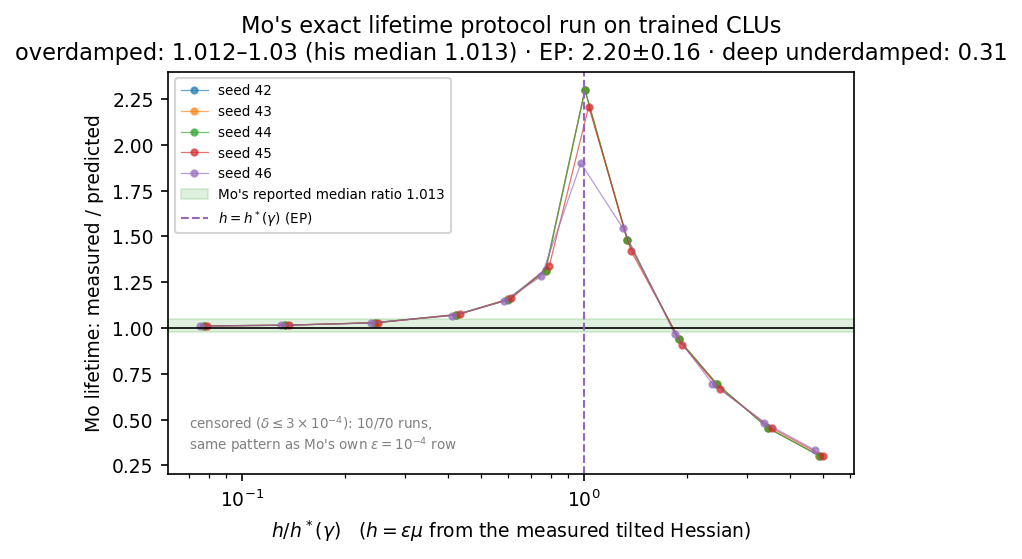
\includegraphics[width=\linewidth]{figs/fig2_mo.png}
\caption{\textbf{Figure 1 (headline).} Mo's single-exponential lifetime law, run \emph{unchanged} on the trained models, is the overdamped face of the mode-mass budget. Measured/predicted lifetime ratio vs. breaking magnitude, $14$ regimes, $5$ seeds: $\approx1$ overdamped (his reported median $1.013$ reproduced), a $2.2\times$ delay spike at the exceptional point, declining to $0.31\times$ deep underdamped --- containment exact below the crossover, failing above it in the calculable ballistic direction. \emph{(Evidence.)}}
\end{figure}

\textbf{3.3 Designed vs. emergent protection, and the price of the physics.} \emph{(Provenance B.1/B.3; tables, controls and full version in Appendix M \S3.4 and Appendices D, H.)} A generic MLP potential trained on perfectly symmetric data develops \emph{no} near-flat direction: softest emergent $\mu^2=5.1/5.9/5.4\!\times\!10^{-2}$ ($3$ seeds) against the designed flat mode $\le2.4\!\times\!10^{-15}$ --- $13$--$14$ orders --- and Mo's own attribution instrument separates the architectures by $15$ orders. Operationally an emergent unit stores nothing on a \emph{continuum}: $\approx1$--$1.6$ bits on $2$--$3$ washboard minima, a written $\delta$ relaxing completely, while the damping-optimum retention law itself still generalizes to that arm (Appendix K, negative N46). \textbf{The price of the prior (evidence).} Against param-matched controls (dim $4$, $150$ ep, $\pm0.05\%$ params, $3$ seeds, same MLP potential) the picture is Pareto, not podium: volume conservation buys bounded (BIBO) dynamics [within the coercive-potential / compact-sublevel-set scope] ($1.00$ vs. $0.33$ for a broken-volume arm), a protected near-flat direction ($\mu^2$ $0.008$ vs. $0.122$) and vacuum survival under contrastive-divergence training ($r^*=0.72$ vs. $0$); leapfrog buys the latch; and the prior costs raw fit --- an unconstrained twin fits $\approx15\times$ better ($0.0128$ vs. $0.190$ eval MSE). That cost is specifically \textbf{\emph{contraction-forbidden} by volume conservation} (the broken-volume arm recovers $\approx2.4\times$ of it precisely by leaking volume), \textbf{not} the causal velocity cap, inactive here. \textbf{The loan is called at $\approx700$ steps (measured):} the twin leads by $1$--$2$ orders to $\approx500$ steps, crosses at $\approx700$ and diverges to $196$ at $5000$, while the unit holds a bounded plateau $\approx0.20$--$0.23$. Its asset is \textbf{boundedness by construction, not the lowest steady MSE} --- broken-volume ($0.14$) and LSTM ($0.13$) plateau below it --- and of the licensed repairs only global damping buys the fit back (a learned friction \emph{field} does not): paid mechanisms are not interchangeable (Appendix H, with the cross-experiment non-comparability caveat its numbers require).

\textbf{3.4 Learned baselines, and the recipe that keeps the vacuum broken.} \emph{(Evidence; provenance B.2/B.4/B.5; tables, overlay figure and full versions in Appendix M \S3.3/\S3.5 and Appendix C, which also carries this result's positioning against the contrastive-divergence literature and its scope clause.)} On Mo's $S^1$ path-integration family the baselines are trained with a learning-rate sweep (best RMSE kept) and are \textbf{not strawmen} --- LSTM and LEM reach train-horizon RMSE $0.18$/$0.23$ rad --- yet under Mo's \emph{autonomous} protocol \textbf{the structural triad (latch, the $\mu^{-2}$ law, bounded drift) is qualitatively absent in them}: coRNN/LEM/LSTM forget the stored analog phase in $\approx5.6/56/69$ map-steps, drift randomizes past $1.2$ rad, and they are \emph{perturbation-fragile} (a $0.1$ hidden kick collapses LSTM $69\to2$, LEM $56\to5$), while the generically-trained unit holds $\approx263$ map-steps with bounded drift ($\approx0.35$ rad, budget law to $+12$--$15\%$) and the designed unit never moves ($5/5$ seeds). \textbf{Honest gap.} The load-bearing claim is the \textbf{qualitative triad, which is architecture- and compute-independent}; the raw $263$-vs-$69$ map-step ratio \textbf{does not survive compute normalization and we retire it as a compute claim} --- per step the Verlet update costs $\approx6.2\times$ an LSTM cell and $\approx3.1\times$ a LEM cell in wall time ($\approx14$--$15\times$ FLOPs, not width-matched), so per unit of retention the unit spends $\approx23.5\times$/$\approx14.6\times$ more wall time than the baselines it out-holds (Appendix I) --- and with no native velocity ingestion it cannot enter Mo's input-driven task-RMSE axis at all, so no task-RMSE was fabricated (N6). \textbf{The designed vacuum also needs a training recipe, because the default one destroys it.} Wake--sleep contrastive divergence drives the order parameter $r^*$ to zero, inverting the designed vacuum in $8/8$ runs at the default $1000$ epochs --- a \textbf{symmetry-restoration (condensate-melting) transition} in the sense of \S2 (the potential lands in the Wigner--Weyl cell, with the predicted degenerate $\mu^2$ pair), on a horizon set by sleep-update \emph{frequency} racing the wake clamp --- chain length immaterial across the two values we run, a within-regime statement (scope clause: Appendix~C) --- and specific to flat/degenerate vacua. A $V(\text{data})$ energy anchor holds the condensate up ($\lambda=100$: $5/5$ seeds, $r^*=0.911\pm0.016$, at the cost of weaker noise rejection and $\approx35\times$ higher wake MSE), and \textbf{every headline law of \S3.1 still holds under it at $\approx20\times$ the erosion horizon} ($3000$ anchored epochs, $3$ seeds: GMOR exact to $1.5\!\times\!10^{-12}$ over $4.6$ decades, slope $-0.956$, same floor, exceptional-point onset bit-identical at $0.5165$). The architecture \emph{breaks} the symmetry, the objective \emph{restores} it, the anchor \emph{keeps it broken}.


\section{Related work}

Neutrality of group-orbit directions is classical (Golubitsky, Stewart \& Schaeffer 1988; Krupa 1990; Rumberger 2001). Closest to us, \textbf{Mo (2026)} proves that a $C^1$ field exactly equivariant under a Lie group has at least $\dim(G/\mathcal H)$ zero Lyapunov exponents tangent to the orbit; we use his diagnostics and his breaking-and-censoring protocol. Our contribution is orthogonal in mechanism (\S3.2): his is the \emph{kinematics} of protection, silent on what sets the gap, whereas here the gap is \emph{constitutive}, and Lyapunov spectra are blind to the write semantics (transport, latch, noise accumulation) that make a neutral direction a \emph{memory}. His theorem is a \textbf{sufficiency} statement; we add the converse-side fact it does not assert: equivariance is \textbf{not necessary}, the latch being a modulus of $V_\theta$ (\S2). Constructive equivariant memory (Di Bernardo et al. 2025; Keller 2025) engineers \emph{which} symmetry a network expresses but does not price \emph{time}: we claim \textbf{no novelty for choosing a symmetry group or coset}, only the price list attached to a chosen structure (see also Iqbal, Keller, Song, Miyato \& Welling 2026). Our learned comparators are LSTM (Hochreiter \& Schmidhuber 1997), LEM (Rusch et al.\ 2022) and coRNN (Rusch \& Mishra 2021a); the conformal-symplectic property of a damped Hamiltonian system is McLachlan \& Perlmutter (2001) and the leapfrog $h<2$ stability limit is standard (Hairer, Lubich \& Wanner 2006); wake--sleep (Hinton et al.\ 1995) and PCD (Tieleman 2008) supply the contrastive objective, and that short-run contrastive divergence distorts an energy landscape is classical (Fischer \& Igel 2010; Nijkamp et al.\ 2020).

\textbf{Retention guarantees elsewhere, and what we therefore do not claim.} They are not this family's exclusive property, and the neighbours are occupied ground we cite rather than claim: HiPPO-LegS (Gu et al.\ 2020) has an $O(tL/\sqrt N)$ approximation bound, a \textbf{polynomial $\Theta(1/t)$, not exponential, gradient decay} and \emph{exact} timescale equivariance with no discretization step to tune --- and we have no measurement saying a learned mass spectrum is preferable to it; location-addressable retrieval of dynamical attractors is published (Kong, Brewer \& Lai 2024); the NTM/DNC lineage was already fully soft, with diagnosed failure modes that transfer (Graves et al.\ 2014, 2016; Csord\'as \& Schmidhuber 2019); tunable permanence is occupied (EDEN, Karuvally et al.\ 2025); and \textbf{UnICORNN} (Rusch \& Mishra 2021b) is Hamiltonian, structure-preserving and \emph{has} the gradient-bound theorem we lack. Our claim is correspondingly narrow: \textbf{a physics-structured associative memory in which retention is a designed, per-item property --- permanent (symmetry-protected, $\mu^2\equiv0$ exactly) or of a finite half-life set by $\mu^2$ --- rather than an emergent consequence of a learned recurrence} --- \emph{controllability}, which we evidence, not \emph{capability}, which we do not claim against transformers or state-space models (nearest published neighbour to this paper's write: \textbf{Titans}, Behrouz et al.\ 2025). \emph{(Full positioning record, the four claims we retire, and the HiPPO challenge in full: Appendix~L.)}


\section{Discussion, limitations, and horizon}

\textbf{Limitations.} All results are laptop-CPU, dim $4$, the $S^1$ testbed, $\le5$ seeds; the solvable core is quadratic and trained statements are local at a critical point of $V_\theta$, with anharmonic deviations quantified (Appendix E). The head-to-head is on \emph{autonomous retention} in map-application units, and the unit does not enter the input-driven task-RMSE axis (\S3.4, N6). BIBO boundedness is evidenced within the coercive-potential / compact-sublevel-set scope and concerns the \textbf{autonomous, designed} setting measured here --- nothing here claims that symplectic structure buys off-distribution stability in a \emph{trained, input-driven} setting, which we do not test and where a published symplectic architecture already holds the ground with a gradient bound (\S4) --- and friction never stabilizes a saddle (Appendix G, N22). The symmetry framing is tree-level only. The finite-$T$ diffusion law holds on \textbf{both} the designed channel (verification) and the emergent arm (evidence, $3$ seeds, above $T^\star\approx3\!\times\!10^{-3}$) under FDT-consistent noise in a Newtonian kinetic mode; the one face that does \textbf{not} generalize is the continuous latch register, which is designed-only (Appendix K, N46).

\textbf{Scope choices, stated so no reader has to infer them.} \textbf{(i) Scale is out of scope by choice:} every number here is dim $4$, hidden $64$, $\le5$ seeds, single-unit, laptop-CPU, and we report \textbf{no} result at larger dimension, wider layers, more units or accelerator scale. \textbf{(ii) No external benchmark is won on its own headline metric anywhere in this paper}; the comparisons are diagnostic retention protocols on a synthetic $S^1$ family and matched-parameter ablations, not leaderboard results --- and \S3.4's honest gap is part of the claim, not a caveat to it. \textbf{(iii) The substrate scope, once, in our own voice: these laws govern the store; end-to-end performance additionally depends on the encoder, measured separately, with its parameter and state-byte budget ledgered.}

\textbf{Horizon and named future work.} The budget suggests reading a trained memory as an \emph{effective field theory of retention}: latches as exact flat directions (moduli of $V_\theta$), registers as pseudo-Goldstone modes of a chosen half-life (a \textbf{designed-geometry} statement; Appendix G, N149/N150), and kinetic isotropy as the price of an equivariant \textbf{write current}, not of the register. Named as directions, not results: the $\mu^{-2}$ law, the crossover and the floor re-measured at latent dimension $\gtrsim64$ and $N\ge8$ interacting units, where mode mixing can break the single-block reduction that makes the budget exact here; the head-to-head on a wider trained-model family; the anchored recipe at longer training and larger width; the equivariant-control wrapper that would put the unit on the supervised task axis; the $(\mu,\gamma,T)$ budget cube whose $T=0$ face is \S3; a learned-store re-test of the explicitly-broken cell that respects the N149/N150 fence; and the price list re-derived for groups beyond abelian $SO(2)$ (a torus $T^2$; the non-abelian $SO(3)\to SO(2)$ coset) --- a direction, on which this paper offers no evidence.


\appendix

\section*{References}
{\small\emph{(Excluded from the venue's main-text page budget. Every record below was verified against the publisher, proceedings or arXiv primary record; preprints are labelled as such.)}\par\medskip
\begingroup
\setlength{\parindent}{-0.22in}\setlength{\leftskip}{0.22in}\setlength{\parskip}{2pt}

Agoritsas, E., Catania, G., Decelle, A., \& Seoane, B. (2023). Explaining the effects of non-convergent MCMC in the training of energy-based models. \emph{ICML}, PMLR 202:322--336. arXiv:2301.09428.\par
Anonymous (2026). \emph{The theory note} (exactly-solvable damped-symplectic retention theory). Anonymized for double-blind review.\par
Behrouz, A., Zhong, P., \& Mirrokni, V. (2025). Titans: Learning to memorize at test time. \emph{NeurIPS 2025}. arXiv:2501.00663.\par
Bhatt, A., Floyd, D., \& Moore, B. E. (2016). Second-order conformal symplectic schemes for damped Hamiltonian systems. \emph{Journal of Scientific Computing} 66(3):1234--1259.\par
Csord\'as, R., \& Schmidhuber, J. (2019). Improving differentiable neural computers through memory masking, de-allocation, and link distribution sharpness control. \emph{ICLR 2019}. arXiv:1904.10278.\par
Decelle, A., Furtlehner, C., \& Seoane, B. (2021). Equilibrium and non-equilibrium regimes in the learning of restricted Boltzmann machines. \emph{NeurIPS 2021}. arXiv:2105.13889.\par
Di Bernardo, A., Valente, A., Mastrogiuseppe, F., \& Ostojic, S. (2025). Shaping manifolds in equivariant recurrent neural networks. arXiv:2511.04802 (preprint).\par
Fischer, A., \& Igel, C. (2010). Empirical analysis of the divergence of Gibbs-sampling-based learning algorithms for restricted Boltzmann machines. \emph{ICANN 2010}, LNCS 6354:208--217. doi:10.1007/978-3-642-15825-4\_26.\par
Fischer, A., \& Igel, C. (2011). Bounding the bias of contrastive divergence learning. \emph{Neural Computation} 23(3):664--673. doi:10.1162/NECO\_a\_00085.\par
Golubitsky, M., Stewart, I., \& Schaeffer, D. G. (1988). \emph{Singularities and Groups in Bifurcation Theory: Volume II}. Applied Mathematical Sciences 69, Springer. doi:10.1007/978-1-4612-4574-2.\par
Graves, A., Wayne, G., \& Danihelka, I. (2014). Neural Turing machines. arXiv:1410.5401 (preprint; never formally published).\par
Graves, A., Wayne, G., Reynolds, M., Harley, T., Danihelka, I., Grabska-Barwi\'nska, A., et al. (2016). Hybrid computing using a neural network with dynamic external memory. \emph{Nature} 538(7626):471--476. doi:10.1038/nature20101.\par
Gu, A., Dao, T., Ermon, S., Rudra, A., \& R\'e, C. (2020). HiPPO: Recurrent memory with optimal polynomial projections. \emph{NeurIPS 2020}. arXiv:2008.07669.\par
Hairer, E., Lubich, C., \& Wanner, G. (2006). \emph{Geometric Numerical Integration: Structure-Preserving Algorithms for Ordinary Differential Equations} (2nd ed.). Springer Series in Computational Mathematics 31.\par
Hinton, G. E., Dayan, P., Frey, B. J., \& Neal, R. M. (1995). The ``wake-sleep'' algorithm for unsupervised neural networks. \emph{Science} 268(5214):1158--1161. doi:10.1126/science.7761831.\par
Hochreiter, S., \& Schmidhuber, J. (1997). Long short-term memory. \emph{Neural Computation} 9(8):1735--1780. doi:10.1162/neco.1997.9.8.1735.\par
Iqbal, N., Keller, T. A., Song, Y., Miyato, T., \& Welling, M. (2026). Spontaneous symmetry breaking and Goldstone modes for deep information propagation. arXiv:2605.14685 (preprint).\par
Jawahar, P., \& Pierini, M. (2026). CHLU: The causal Hamiltonian learning unit as a symplectic primitive for deep learning. arXiv:2603.01768 (short paper, ICLR 2026 AI \& PDE workshop).\par
Jelassi, S., Brandfonbrener, D., Kakade, S. M., \& Malach, E. (2024). Repeat after me: Transformers are better than state space models at copying. \emph{ICML}, PMLR 235:21502--21521. arXiv:2402.01032.\par
Karuvally, A., Lertsaroj, P., Sejnowski, T. J., \& Siegelmann, H. T. (2025). Exponential dynamic energy network for high-capacity sequence memory (EDEN). \emph{NeurIPS 2025}. arXiv:2510.24965.\par
Keller, T. A. (2025). Flow equivariant recurrent neural networks. \emph{NeurIPS 2025} (spotlight). arXiv:2507.14793.\par
Kong, L.-W., Brewer, G. A., \& Lai, Y.-C. (2024). Reservoir-computing based associative memory and itinerancy for complex dynamical attractors. \emph{Nature Communications} 15:4840. doi:10.1038/s41467-024-49190-4.\par
Krupa, M. (1990). Bifurcations of relative equilibria. \emph{SIAM Journal on Mathematical Analysis} 21(6):1453--1486. doi:10.1137/0521081.\par
McLachlan, R. I., \& Perlmutter, M. (2001). Conformal Hamiltonian systems. \emph{Journal of Geometry and Physics} 39(4):276--300.\par
Mo, H. H. (2026). Symmetry-protected Lyapunov neutral modes in equivariant recurrent networks. arXiv:2605.03338 (preprint; single author).\par
Nijkamp, E., Hill, M., Han, T., Zhu, S.-C., \& Wu, Y. N. (2020). On the anatomy of MCMC-based maximum likelihood learning of energy-based models. \emph{AAAI 2020}. arXiv:1903.12370.\par
Ramsauer, H., Sch\"afl, B., Lehner, J., Seidl, P., Widrich, M., Adler, T., et al. (2021). Hopfield networks is all you need. \emph{ICLR 2021}. arXiv:2008.02217.\par
Rumberger, M. (2001). Lyapunov exponents on the orbit space. \emph{Discrete and Continuous Dynamical Systems} 7(1):91--113. doi:10.3934/dcds.2001.7.91.\par
Rusch, T. K., \& Mishra, S. (2021a). Coupled oscillatory recurrent neural network (coRNN): An accurate and (gradient) stable architecture for learning long time dependencies. \emph{ICLR 2021}. arXiv:2010.00951.\par
Rusch, T. K., \& Mishra, S. (2021b). UnICORNN: A recurrent model for learning very long time dependencies. \emph{ICML}, PMLR 139:9168--9178. arXiv:2103.05487.\par
Rusch, T. K., Mishra, S., Erichson, N. B., \& Mahoney, M. W. (2022). Long expressive memory for sequence modeling. \emph{ICLR 2022}. arXiv:2110.04744.\par
Tieleman, T. (2008). Training restricted Boltzmann machines using approximations to the likelihood gradient. \emph{ICML 2008}, 1064--1071. doi:10.1145/1390156.1390290.\par
Toledo-Mar\'in, J. Q., Maiti, A., Fox, G. C., \& Melko, R. G. (2025). Exploring the energy landscape of RBMs: Reciprocal space insights into bosons, hierarchical learning and symmetry breaking. \emph{Machine Learning: Science and Technology} 6(3):035030. arXiv:2503.21536.\par
\endgroup}

\emph{Cross-reference convention for the appendix block: section numbers of the form \S N.M cited in Appendices A--L are the \textbf{long-form} numbering, i.e.\ the sections of Appendix~M (the pre-condensation main text). The condensed main text carries the same material in \S2--\S3.4; where a pointer matters, the appendix names Appendix~M explicitly.}

\section{An $SO(2)$ symmetry-breaking primer for machine-learning readers}

\emph{(Expository, and deliberately the first thing in the appendix block. It restates, for a reader with no field-theory background, the classical argument behind the axis-1 taxonomy of \S2. It contains \textbf{no new result and no claim of its own}: \S2 remains this paper's controlling definition of spontaneous symmetry breaking, and every quantitative statement lives in \S3 or in Appendices B--K. Symbols follow this paper's conventions, which differ from the usual pedagogical letters --- notation map in A.6. Adapted from a co-author's tutorial note; the attribution is deliberately non-identifying under double-blind review and the acknowledgement is placed in the camera-ready.)}

\begin{quote}\small
\textbf{Scope note --- four clauses that bind every sentence of this appendix.}

\textbf{(i) Designed, exact-$SO(2)$ potentials only.} The neutral direction described below is \textbf{designed exact $SO(2)$ only --- the emergent arm has no coset register} (negative N46, Appendix G; evidence, $3$ trained MLP seeds, dim $4$). On trained emergent (MLP) potentials the direction of largest coset overlap is a middle-of-spectrum \emph{massive} mode, only $1.7$--$4.9\times$ softer than the \emph{stiffest} Hessian mode; a written $\delta\in\{0.1,0.3,0.5\}$ rad relaxes completely ($|{\rm retained}|\le2.1\!\times\!10^{-3}$); capacity is $\approx1$--$1.6$ bits on $2$--$3$ washboard minima, not a real-valued continuum (Appendix K.1). Nothing in this primer licenses reading ``flat direction'' onto a generically-trained potential.

\textbf{(ii) $T=0$.} The infinite half-life is a statement about the \emph{deterministic} damped map. At $T>0$ --- under the Langevin sampler --- the coset coordinate performs a random walk with diffusion constant $D_\theta=\varepsilon T(2-\gamma)/(2F^2\gamma)$, $F^2=M_{\rm ch}r^{*2}$, so the register has a finite, computable lifetime $n_{1/2}\propto F^2\gamma/(\varepsilon^2T)$ and is a \emph{diffusive register}, not long-range order (\S2; measured in Appendix K.2, whose mandatory \texttt{langevin\_noise="fdt"} \textbf{and} Newtonian-kinetic-mode flag travels with every number there).

\textbf{(iii) Storage additionally requires $\gamma>0$.} A flat direction alone gives \emph{neutrality}, not storage: at $\gamma=0$ the flat mode is a marginal drifting integrator (a write never freezes). Any $\gamma>0$ converts it into an exact latch --- a momentum impulse $p_0$ writes the finite displacement $\varepsilon p_0/(M\gamma)$ and the stored value then persists with infinite half-life (\emph{theory note}, latch theorem; verified in \S3.1).

\textbf{(iv) Pedagogy, with attribution --- not a contribution.} That group-orbit directions are neutral is classical, and in the machine-learning setting it has recently been stated for equivariant recurrent flows: Mo (2026) proves that such a flow has \textbf{at least} $\dim(G/\mathcal H)$ zero Lyapunov exponents along the group orbit. We cite it here and claim nothing. Equivariance is moreover \textbf{sufficient but not necessary} for a neutral memory direction --- we exhibit a measured non-equivariant counterexample that latches (\S3.4, Appendix D, \S4).
\end{quote}

\textbf{A.1 The object.} We follow the latent position $q$ and assume a two-dimensional latent space. ``Two-dimensional'' here means the \textbf{channel plane} of a trained unit, not the unit itself: the trained units of this paper are dim $4$, of which two coordinates carry the $SO(2)$ channel and the rest are spectators (\S2). The relevant symmetry group is $SO(2)$, whose elements are the two-dimensional rotations by an angle $s$, acting as $q\mapsto R(s)\,q$ with $R(s)$ the rotation matrix. The potential is symmetric under $SO(2)$ when

\begin{equation}
V\big(R(s)\,q\big)=V(q)\qquad\forall\,s.
\end{equation}

A potential satisfying (A.1) is therefore one with radial dependence only, $V\equiv V(r)$.

\textbf{A.2 Two realizations of the symmetry.} \emph{(Two cases, which is what typically occurs and what the potentials of this paper realize; an invariant potential can also present both structures at once --- a critical point at the origin \textbf{and} a degenerate ring --- in which case the argument below is applied at whichever vacuum the trained model actually occupies.)} If the minimum of the potential is at the origin, $r^*=0$, the minimizer is unique and trivially invariant, $q^*=(0,0)$ with $R(s)\,q^*=q^*$: this is the \textbf{unbroken}, or \textbf{Wigner--Weyl}, realization. The other case is a potential with degenerate minima at $r^*>0$. Then a whole \emph{set} of vacua minimizes the potential, $q^*=r^*(\cos\theta_0,\ \sin\theta_0)$ for every vacuum angle $\theta_0$, and the vacuum is in general \textbf{not} invariant, $R(s)\,q^*\neq q^*$, while (A.1) still holds and $R(s)\,q^*$ has the same potential energy as $q^*$. Choosing one vacuum out of a degenerate set is \textbf{spontaneous symmetry breaking}: the system is invariant under the group $G$, but its ground state is invariant only under a subgroup $\mathcal H\subset G$ (here the trivial subgroup). There is \textbf{one Nambu--Goldstone mode per broken generator}, and the NG fields parametrize the coset space $G/\mathcal H$, whose dimension equals the number of broken generators ($1$ for $SO(2)$ fully broken).

\textbf{A.3 Why the broken realization gives a zero spectral mass.} The \emph{group elements} of $SO(2)$ are the rotations $R(s)$; its \emph{Lie algebra} is $\mathrm{span}\{X\}$, spanned by the single generator $X$ of infinitesimal rotations, and $R(s)=e^{sX}$. The vacuum condition is stationarity along the whole orbit,

\begin{equation}
\nabla V\big(R(s)\,q^*\big)=0\qquad\forall\,s,
\end{equation}

since every $e^{sX}q^*$ is another vacuum; the tangent vector to the vacuum orbit at $q^*$ is $Xq^*$. Differentiating (A.2) with respect to $s$ and evaluating at $s=0$ gives

\begin{equation}
\nabla^2V(q^*)\,Xq^*=0.
\end{equation}

In other words $Xq^*$ is an eigenvector of the Hessian at the vacuum with eigenvalue \textbf{zero} --- the Goldstone direction. Heuristically, moving along the orbit tangent costs no energy because the potential has no curvature across it. The analogy to particle physics is then apparent: spontaneous symmetry breaking gives rise to massless Goldstone bosons as a result of the flat direction in the potential, whereas in the machine-learning context it produces a \textbf{neutral direction in which information can be stored without being pulled back} --- subject, in full, to clauses (i)--(iv) of the scope note above (designed $SO(2)$ potentials; $T=0$; $\gamma>0$ to freeze the write; and published kinematics, not a contribution of ours).

\textbf{A.4 Bare Hessian vs. mass-whitened Hessian (a convention the reader must carry).} Equation (A.3) is a statement about the \textbf{bare} Hessian $\nabla^2V_\theta(q^*)$. This paper's \textbf{spectral mass} is the eigenvalue of the \emph{mass-whitened} Hessian, $\mu_k^2=\lambda_k\big(M_{\rm eff}^{-1/2}\nabla^2V_\theta M_{\rm eff}^{-1/2}\big)$ (\S1, Nomenclature). The two agree exactly \emph{for the zero mode}: by Sylvester's law of inertia, congruence by any invertible $M_{\rm eff}$ preserves the rank and inertia of the Hessian, so a bare zero stays a whitened zero for every inertial anisotropy (the null \emph{direction} rotates to $M_{\rm eff}^{1/2}Xq^*$, and massive eigenvalues are rescaled). So A.3's $\mu^2=0$ transfers verbatim to this paper's convention --- but any \emph{quantitative} extension of the argument (GMOR, retention half-lives) must whiten, or its numbers will not match \S3.1 or Appendix J.

\textbf{A.5 The unbroken case, stated precisely.} <!-- FLAG (v0.7, task v2-revision-6 item 2): the wording of this paragraph's first sentence is the corrected form recommended by the theory audit (the original tutorial text read ``doesn't give a zero spectral mass'', which is false as an implication). It AWAITS THE CO-AUTHOR'S SIGN-OFF via the Head before this appendix is printed. -->The same argument \textbf{does not \emph{force}} a zero spectral mass in the unbroken realization: the vacuum is unique, $q^*=0$, so $Xq^*$ is trivial and \textbf{the orbit argument degenerates, giving no information about the eigenvalue}. What holds generically --- at a \emph{nondegenerate} invariant minimum --- is $\mu^2>0$, degenerate within each irreducible representation by Schur's lemma (\S2; the taxonomy table itself is row 1 of Appendix~M \S2.1). The distinction is not pedantry: an invariant potential can have a unique, invariant minimizer \emph{and} a vanishing Hessian there (e.g. $V=r^4$ at the origin), i.e. $\mu^2=0$ with no symmetry breaking at all. ``Unbroken'' therefore predicts \emph{no protection argument}, not \emph{no flat direction}.

\textbf{A.6 Notation map (this paper vs. the usual pedagogical letters).} Four symbols are re-lettered here because the usual choices collide with load-bearing conventions of this paper and of the theory note.

\begin{center}\small
\begin{tabular}{@{}l p{1.3in} p{1.0in} p{2.6in}@{}}
\toprule
primer symbol (here) & meaning & letter used in most textbook treatments & why it is not used here \\
\midrule
$s$ & group parameter (rotation angle), $R(s)=e^{sX}$ & $\alpha$ & $\alpha$ is the confinement coefficient of the learned-store battery quoted in Appendix~G (N149/N150) \\
$X$ & the $SO(2)$ generator & $J$ & $J$ is the map Jacobian throughout (\S2: $J^\top\Omega J=(1-\gamma)\Omega$, $\det J=(1-\gamma)^d$) \\
$\theta_0$ & the vacuum angle labelling a point on the orbit & $\omega$ & $\omega$ is a mode frequency ($\omega_k=\mu_k$) in the theory note; $\theta$ is the \emph{stored} coset coordinate \\
$\mathcal H$ & the unbroken subgroup, $\mathcal H\subset G$ & $H$ & $H=T(p)+V_\theta(q)$ is the Hamiltonian \\
\bottomrule
\end{tabular}
\end{center}

\textbf{A.7 What this primer does not cover.} It stops at the exactly-massless (Nambu--Goldstone) case and is silent on the third realization --- the \textbf{pseudo-Goldstone} cell, which is where the mode-mass budget of \S3 actually lives. The taxonomy of \S2 is strictly more complete, and \S2's finite-dimensional, tree-level definition (no thermodynamic limit, no $\hbar$) together with its ``what we do not import'' paragraph governs the whole paper. The method above does extend to explicit breaking by differentiating the \emph{tilted} stationarity condition --- that is how \S3.1's $\mu^2\propto\delta$ law and Appendix J's GMOR-proper identity arise --- but the extension carries its own scope, including the learned-store tilt refutation recorded in Appendix G (N149/N150): on a learned multi-atom store an explicit-breaking coefficient moved the softest eigenvalue \emph{the wrong way}, so the tilt is a designed-geometry construction here and not a general lifetime dial.
\label{app:primer}

\section{Flag-provenance tables}\label{app:flags}
\sloppy\small
\emph{Every training-config-sensitive result inherits its full flag set (from the source reports) so no cross-section contradiction can be constructed.}

\textbf{B.1 Trained models (designed \& emergent).} Base code \texttt{main@dbeb2c2} (ckpts), probes \texttt{@db3369b}. \texttt{ExperimentDConfig}: dim $4$, hidden $64$, \texttt{newtonian\_learned}, \texttt{tie\_channel\_mass=True} (designed/emergent) or \texttt{False} (broken-iso, App.~D), $\mathrm{dt}=0.05$, circle $R{=}1.0{\times}256$, window $64$; \texttt{train\_epochs=150}; \texttt{lyapunov\_penalty="max"} ($\lambda{=}0.01$), \texttt{langevin\_noise="legacy"}, \texttt{persistent\_sleep\_buffer=False}, \texttt{sleep\_temperature=0.5}, \texttt{sleep\_frequency=5}, \texttt{sleep\_friction=0.0}, lr $10^{-3}$, batch $64$, clamp $1000{\to}1$ ramp $0.5$. Seeds: designed $\{42$--$46\}$, emergent $\{42$--$44\}$. Potentials: \texttt{so2\_invariant} / \texttt{mlp}. Probes: x64, damped settle $\gamma{=}0.1{\times}4000$ + BFGS ($|\nabla V|{\to}10^{-9}$--$10^{-14}$), probe $\gamma{=}0.05$, kick $0.1$; floor $27.03$ steps.

\textbf{B.2 Learned baselines.} Scratch \texttt{@db3369b}. coRNN/LEM/LSTM hidden $16$; train seq-len $64$, test $256$; Adam; lr $\in\{10^{-3},3{\times}10^{-3},10^{-2}\}$ swept, best-RMSE kept; $\omega\sim\mathcal N(0,0.3)$; coRNN $\mathrm{dt}{=}0.1,\gamma{=}\varepsilon{=}1.0$; LEM $\mathrm{dt}{=}1.0$; MSE; retention: write-len $32$, hold $2000$, $64$ writes, threshold $0.2$~rad, perturbation $\sigma{=}0.1$; seeds $\{42$--$46\}$.

\textbf{B.3 Minus-the-physics.} \texttt{main@db3369b}, code @ \texttt{b41410f}. Seeds $\{42,43,44\}$, $150$ ep, dim $4$, hidden $64$, \texttt{newtonian\_learned}, potential \texttt{mlp} (identical across arms), $\mathrm{dt}{=}0.05$, $R{=}1.0{\times}256$, seq-len $65$; lr $10^{-3}$, batch $64$, \texttt{lyapunov\_penalty="max"}, \texttt{langevin\_noise="legacy"}, \texttt{sleep\_friction=0.0}; twin hidden $59$ (param-matched), broken-volume $\log$-scale init $0$.

\textbf{B.4 Erosion \& anchor.} Bit-faithful \texttt{train\_chlu} replica (max$|\Delta\text{param}|{=}0$ vs.\ \texttt{run\_experiment\_d}). Swept: \texttt{sleep\_frequency}$\in\{1,5,20\}$, \texttt{sleep\_steps}$\in\{50,500\}$, \texttt{persistent\_sleep\_buffer}$\in\{F,T\}$, \texttt{sleep\_friction=0.0}; anchor $\lambda\in\{0,1,10,100\}$, target $=$ epoch-0 mean $V(\text{ring})$; epochs $\{1000,3000\}$, seeds $\{42$--$46\}$.

\textbf{B.5 Referee-experiment additions} (\texttt{v2-referee-experiments}, repo \texttt{main@37dc664}, read-only). \emph{SF-1} (Mo-estimator overlay, \S3.2 / Fig.~\ref{fig:mo_own}): extraction from \texttt{v2-full-runs/gmor\_sweep.npz} (commit \texttt{dbeb2c2}; the B.1 designed battery, \texttt{train\_epochs=150}, seeds $\{42$--$46\}$); predictor $=\hat\lambda(T{=}128)$ via \texttt{probe\_common.group\_tangent\_exponent}, seed $\Xi=(Xq^*,0)$; lifetime predictor $=0.847298/\text{rate}$, rate $=-\,$\texttt{lam\_hat\_128}. No retraining. \emph{SF-2} (per-step compute, \S3.3 / App.~I): commit \texttt{37dc664}, f32. CLU $=$ \texttt{build\_exp\_d(42, potential\_type="mlp")} (the $263$-step emergent arch), $\gamma{=}0.05$, $\mathrm{dt}{=}0.05$, KDK $=$ two $\nabla_qV$ backprops through a dim-$4{\to}64{\to}64{\to}1$ tanh MLP, \texttt{newtonian\_learned}. Baselines LSTM/LEM cells in$=1$/hidden$=16$/out$=2$ (the B.2 models). FLOPs via XLA \texttt{cost\_analysis()}; wall $=$ median of $7$ reps of a \texttt{lax.scan} of $2{\times}10^5$ steps (dispatch-amortized; single-call timing is dispatch-bound and \emph{not} reported). Seeds do not affect FLOP/timing. \emph{SF-3} (laws survive the cure, \S3.5 / App.~C.7): commit \texttt{37dc664}; \texttt{so2\_invariant}, \texttt{tie\_channel\_mass=True}, \texttt{anchor\_lambda=100} (target $=$ mean $V(\text{ring})$, anchor data $=$ ring $q$), \texttt{train\_epochs=3000}, seeds $\{42,43,44\}$; \texttt{sleep\_frequency=5}, \texttt{sleep\_steps=500}, \texttt{persistent\_sleep\_buffer=False}, \texttt{sleep\_friction=0.0}, \texttt{lyapunov\_penalty="max"}, \texttt{langevin\_noise="legacy"}, $\mathrm{dt}{=}0.05$, \texttt{newtonian\_learned}; driver $=$ \texttt{sleep-erosion-study/driver.py::train\_checkpointed} $+$ anchor ($132$~s/model, f32 CPU); probe x64 ($\gamma{=}0.05$, kick $0.1$, tilt $n{=}1$, $\delta\in\{10^{-4}$--$4\}$). Cross-check: seed-42 wake loss $0.06102$ reproduces \texttt{anchor-robustness} \texttt{chlu\_l100\_s42} to $5$ digits.

\textbf{B.6 GMOR proper --- condensate-resolving spurion} (\texttt{f1-gmor-condensate}, Appendix~\ref{app:gmor}). Code @ \texttt{9bc2cf7} (base \texttt{main@27f232f}). \textbf{Probe-only, no retraining.} Checkpoints: \texttt{designed150\_s\{42--46\}} (the B.1 designed battery: \texttt{so2\_invariant}, \texttt{newtonian\_learned}, \texttt{tie\_channel\_mass=True}, \texttt{tilt\_delta=0}, \texttt{sleep\_mode=on}, $150$ ep) and \texttt{anchored3000\_s\{42,43,44\}} (same $+$ anchor $\lambda{=}100$, $3000$ ep --- the B.5/SF-3 checkpoints). Spurion: \texttt{LinearSpurionPotential}, $V\to V-\delta(u\cdot q)$, $u=$\texttt{channel\_spurion\_direction(4,0.0)}$=e_0$ (direction check also at angles $0.7$, $-2.3$); $\delta\in\{10^{-8},10^{-7},10^{-6},10^{-5},10^{-4},10^{-3},10^{-2},3{\times}10^{-2},10^{-1},3{\times}10^{-1}\}$. \textbf{Defaults \texttt{spurion\_delta=0.0} $\Rightarrow$ no wrapper constructed $\Rightarrow$ every other result in this paper is bit-compatible.} Precision \texttt{jax\_enable\_x64=True} (f32-trained weights cast to f64); JAX $0.9.0$, equinox $0.13.4$, main venv. Vacuum solve: Newton on $u\cdot\nabla V_{\rm base}=\delta$ (residual $\le4.4{\times}10^{-16}$), cross-checked structure-agnostically by BFGS polish of the full spurioned potential ($|r^*_{\rm BFGS}-r^*_{\rm Newton}|=0.0$ bit-identical, $|\nabla V|_{\rm BFGS}\le2.6{\times}10^{-13}$). $\Sigma_{\rm FD}$ step $h{=}10^{-6}$, central, $\delta\ge10^{-4}$ only. \textbf{Not swept:} $\mathrm{dt}$, $\gamma$, kinetic mode --- this probe touches only $V$ and its Hessian (no rollouts, no integrator). Per-checkpoint constants ($\delta{=}0$): $f=\Sigma(0)\in[0.9086,0.9907]$, $M_{\rm ch}\in[0.2310,0.6875]$, $F^2(0)\in[0.1907,0.6748]$, $\mu_{\rm rad}^2\in[0.6703,6.3158]$, flat $\mu^2\in[-1.3{\times}10^{-15},2.2{\times}10^{-15}]$.

\textbf{B.7 Finite-temperature coset diffusion} (\texttt{t-lever-forgetting}, Appendix~\ref{app:tcube}). Repo \texttt{27f232f}$\to$\texttt{9bc2cf7} (depended-on code paths verified byte-identical across the move; headline cell re-run bit-identical). Checkpoints \texttt{designed150\_s\{42--46\}} (B.1 designed battery), \textbf{re-tied} (\texttt{tie\_channel\_mass} folded into \texttt{log\_mass}; $H$ bit-identical, pytree-level only, no repo edit). \textbf{\texttt{langevin\_noise="fdt"} everywhere} ($\triangle$ repo default is \texttt{legacy}; none of the Appendix-\ref{app:tcube} laws hold under it). \texttt{friction\_field}/\texttt{temperature\_field} $=$ \texttt{none}; \texttt{tilt\_delta=0}, \texttt{spurion\_delta=0} (unbroken, exact Goldstone); $\varepsilon=\mathrm{dt}=0.05$; $\gamma$ grids $\{0.005,0.01,0.02,0.05,0.1,0.2\}$, $\{0.01,0.02,0.05,0.1,0.2\}$, dense \texttt{geomspace(0.002,0.5,22)}; $T\in\{0,10^{-4},3{\times}10^{-4},10^{-3},3{\times}10^{-3},10^{-2}\}$ (exponents quoted only for $T\le3{\times}10^{-3}$, linear response). Precision float64 (\texttt{jax\_enable\_x64}; training was f32). Seeds $42$--$46$; PRNG keys derived per $(\text{seed},T,\gamma)$. Env: JAX $0.9.0$, equinox $0.13.4$, numpy $2.4.1$, scipy $1.17.0$, main venv.

\medskip
\textbf{B.8 Emergent-arm forgetting generalization} (\texttt{v5-gate}, Appendix~\ref{app:tcube}'s emergent evidence --- K.1's negative N46, K.4's V-curve and $T^\star$). Repo \texttt{d6f8bac} (the FDT-inertia fix committed mid-session; \textbf{all runs use \texttt{common.retie(model)}}, under which \texttt{effective\_mass()}$\equiv$\texttt{effective\_inertia()} --- verified $\max|{\rm eff\_mass}-{\rm eff\_inertia}|=0$ on all checkpoints, so every number is invariant to the fix). Checkpoints \texttt{emergent150\_s\{42,43,44\}} (\texttt{potential\_type="mlp"}) $+$ \texttt{designed150\_s44} (matched control), otherwise the B.1 Experiment-D config (dim $4$, hidden $64$, \texttt{newtonian\_learned}, \texttt{tie\_channel\_mass=True}, $150$ ep). \textbf{\texttt{langevin\_noise="fdt"} everywhere} (repo default \texttt{legacy}, under which none of the laws hold); \textbf{re-tied}; \texttt{friction\_field}/\texttt{temperature\_field}/\texttt{tilt\_delta}/\texttt{spurion\_delta} all off for the coset probes. $\varepsilon=\mathrm{dt}=0.05$; \textbf{$\Delta=0.5$~rad} --- every emergent $n_{1/2}$ is at this coset tolerance (never quote without $\Delta$ and $\ell_\theta/\Delta$). Jacobian $\gamma$-grid \texttt{geomspace(0.002,0.5,48)}; $T$-sweep $\gamma\in\{0.01,0.05,0.2\}$, $T\in\{2,4,8,16,32\}{\times}10^{-3}$, $96$ walkers, cap $150000$ ($60000$ designed control); $0/45$ cells censored. Precision float64 (\texttt{jax\_enable\_x64}; weights f32$\to$f64). Model seeds as listed; PRNG per $(\text{seed},T,\gamma)$. Env: JAX $0.9.0$, equinox $0.13.4$, numpy $2.4.1$, scipy $1.17.0$, main venv. Harness cross-check: reproduces \texttt{t-lever-forgetting}'s matched designed cell ($n_{1/2}=1690$ vs $1600$, $5.6\%$, within the per-cell statistical error).

\medskip
\textbf{B.9 The learned-store tilt/lifetime battery} (Appendix G, N149/N150 --- the only numbers in this paper that come from a \emph{different} architecture, quoted solely to fence this paper's designed-geometry tilt results). Code @ \texttt{647c54e} (4 commits off \texttt{1ce02e4}); ⚠ the measured cells were run on \texttt{main @ 233fd9e} and the branch rebased afterwards, with the summary card re-emitted from saved records (no re-run) --- disclosed, and the control arm reproduces its reference harness exactly. Env: main venv, JAX $0.9.0$, equinox $0.13.4$ (no worktree re-sync). Store: a learned atom-dictionary potential with shell atoms, confinement $\alpha=0.05$, atom init width $0.3$, depth init $10^{-4}$; geometry unmodified from its harness defaults (dim $4$--$6$, $K=6$, $192$ atoms in the primary family). Breaking dial: rank-$1$ per-group tilt, learned direction, $\epsilon\in\{0,10^{-3},10^{-2},10^{-1},1,10\}$ (pre-registered; $\epsilon=10$ the destructive anchor), two breaking weights (envelope / depth), radius frozen on the tilt arms. Write: $300$ steps, AdamW lr $3\!\times\!10^{-3}$, wd $10^{-4}$, $32$ perturbations, $\sigma_{\rm addr}=0.25$, $\sigma_{\rm pay}=0.6$, margin $0.15$, barrier $0.2$. Read/probe: $\mathrm{dt}=0.05$, $\gamma_{\rm read}=0.02$ ($\Rightarrow\Gamma=\gamma/\mathrm{dt}=0.4$), \texttt{newtonian\_learned}; $\tau$ probe = displacement $0.1$ along the softest eigenvector, $4000$ steps, decay rate fitted on the monotone upper envelope over $[0.92c_0,0.03c_0]$, median over $\le4$ sites. \textbf{Seeds: $\{0,1,2\}$ on the race cells; ⚠ the $\epsilon$-dial sweep and the low-confinement extra are seed $0$ only and are labeled as such wherever quoted.} $T=0$, $p_0=0$, no Langevin, no wake--sleep --- this battery shares no training configuration with the trained units of \S3, which is precisely why it is quoted as a scope fence and never as a measurement of the units in this paper.

\section{The erosion study: law and cure (full)}\label{app:erosion}
\emph{Positioning (literature search completed 2026-08). Landscape distortion under short-run contrastive divergence is itself classical (Fischer \& Igel 2010, 2011; Nijkamp et al.\ 2020); what this appendix adds is \textbf{(i)} a measured, quantified \textbf{inversion} of a \emph{designed, symmetry-degenerate} vacuum on a symplectic energy-based unit --- a sharp instance on a known substrate, not the discovery that CD is biased; \textbf{(ii)} the \textbf{degeneracy-specificity demarcation} (a designed vacuum is eroded iff it has a flat direction the wake objective cannot see); and \textbf{(iii)} the \textbf{frequency-set erosion horizon}. A targeted search of the CD/EBM, continual-EBM, equilibrium-propagation and RBM-symmetry-breaking literatures (arXiv cs.LG / cs.NE / cond-mat.dis-nn / stat.ML through Aug 2026; NeurIPS 2020--2025, ICML/PMLR v119/v139/v202/v235, ICLR/OpenReview, AAAI; \emph{Neural Computation}, \emph{Machine Learning: Science and Technology}, \emph{Frontiers in Computational Neuroscience}, \emph{Mathematics}, \emph{Nature Communications}) found no prior statement of (ii) or (iii). \textbf{That is absence over the surfaces listed, not proof of none:} paywalled journal archives, forward-citation crawls of the CD-bias literature, non-English work and workshop tracks were not searched. \textbf{Scope clause for (iii), which travels with it.} The nearest documented neighbour concerns \emph{chain length}: in RBM/EBM learning the number of sampling steps $k$ relative to the model's mixing time defines equilibrium vs.\ out-of-equilibrium learning regimes and does change what is learned (Decelle, Furtlehner \& Seoane 2021; Agoritsas et al.\ 2023). Our sweep varies chain length only over \texttt{sleep\_steps}$\in\{50,500\}$ at otherwise fixed sampler settings and does not resolve where either sits relative to this model's mixing time, so the finding is \emph{frequency-decisive across the two chain lengths we run}, and is \textbf{not} a claim that chain length is irrelevant to contrastive-divergence learning in general. Relatedly, the nearest RBM symmetry-breaking result attributes the breaking to hierarchical feature learning rather than to the CD update (Toledo-Mar\'in et al.\ 2025), so it is not a precedent for (i) either. Placement (methods appendix vs.\ standalone section) is a pending editorial decision. Registry: N5.}
\textbf{C.1 Phase diagram} (seeds $\{42,43\}$): ring forms by $\approx100$ ep (depth $-0.11\to+0.079$) then erodes. Inversion epoch by sleep frequency: $116$ (f1) / $442$ (f5) / $959$ (f20); \texttt{sleep\_steps} $50\equiv500$; PCD vs.\ CD $\le9$~ep. \textbf{C.2 Mechanism}: in-ring-band negative fraction $0.22$--$0.31\to0.03$--$0.11$; negative mean energy $3.4\to12.3$; negative radius $1.45\to3.9$ (overlap$\to$raise$\to$expel). \textbf{C.3 Cure}: baseline depth $-0.126$, $r^*{=}0$, noise-gap $-0.028$; anchor $\lambda{=}10$ depth $+0.069$, $r^*{=}0.96$, gap $+0.244$ ($>$ wake-only $+0.199$); $H$-gating fails. \textbf{C.4 Envelope} ($5$ seeds, $3000$ ep): $\lambda{=}100$ bulletproof ($5/5$, $r^*{=}0.911\pm0.016$); $\lambda{=}10$ gap $1.8$ but $1/5$ collapses; $\lambda{=}0$ dies. \textbf{C.5 Demarcation}: tilt $\delta\ge0.05$, $\lambda{=}0$ immunizes; non-degenerate sine immune. \textbf{C.6 Cross-link}: anchor does not rescue broken-volume (diverges; wake MSE $3.5$k--$176$k); CD-robustness is a volume-conservation payoff, orthogonal to the anchor. Silent knob (N19): \texttt{sleep\_temperature} no-op at \texttt{sleep\_friction=0}.

\textbf{C.7 The headline laws survive the cure at $3000$ ep} (\texttt{v2-referee-experiments} SF-3; anchored $\lambda{=}100$, $3$ seeds $\{42,43,44\}$, $\approx20\times$ the default-$1000$-ep erosion horizon; provenance B.5). Vacuum intact: ring depth $+0.106/+0.101/+0.124$ (a well, not a max), $r^*=0.925/0.909/0.918$ (mean $0.917\pm0.007$, matching \texttt{anchor-robustness} $0.911\pm0.016$), flat-mode $\mu^2=-7.6{\times}10^{-16}/-1.3{\times}10^{-15}/+2.2{\times}10^{-15}$ (machine-flat), angular overlap $1.0000$. \textbf{GMOR exact}: $\mu^2_{\rm meas}/[\delta n^2/(M_{\rm ch}r^{*2})]=1.00000\pm{\le}1.5{\times}10^{-12}$ at every $\delta$, all $3$ seeds, over $4.6$ decades. \textbf{Retention}: overdamped slope $-0.956$ (predicted $-1$; cf.\ $150$-ep $-0.985$, GMOR ratio still exactly $1$); floor $27.03$ ($n_{1/2}$ $24$--$31$ straddling within the kick-phase ripple); latch preserved ($\mu^2\approx10^{-15}\Rightarrow\infty$). \textbf{EP}: $\varphi=0$ exactly below (max freq$_{\rm jac}=0.000\mathrm{e}{+}00$, all seeds); above, slope $0.5165$ (predicted $0.5$) --- \textbf{bit-identical to the $150$-ep value}. Every headline law of \S3.1 survives past the erosion horizon under the shipped anchor cure.

\begin{figure}[t]\centering
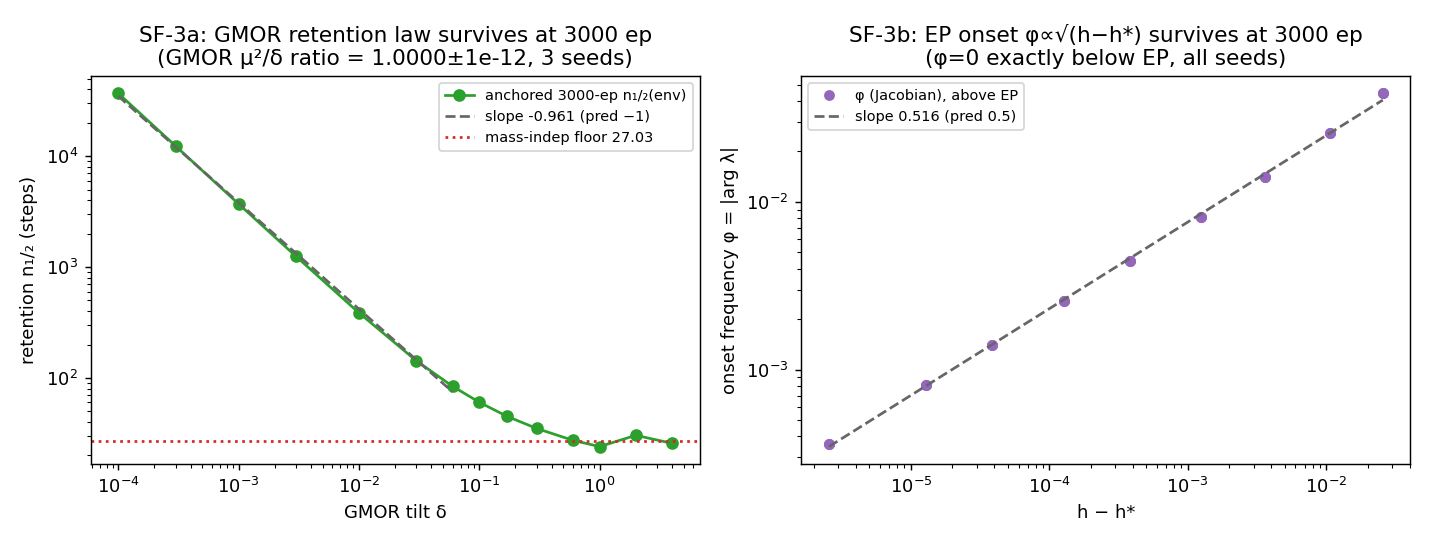
\includegraphics[width=\textwidth]{figs/sf3_anchored3000_laws.png}
\caption{The \S3.1 headline laws survive the shipped anchor cure at $3000$ epochs ($\approx20\times$ the erosion horizon; anchored $\lambda{=}100$, $3$ seeds). Left: the GMOR retention law $n_{1/2}$ vs.\ tilt $\delta$ --- anchored-$3000$-ep points on the predicted slope (fitted $-0.961$, predicted $-1$) saturating at the mass-independent floor $27.03$; $\mu^2/\delta$ ratio $1.0000\pm10^{-12}$ over $4.6$ decades. Right: the exceptional-point onset $\varphi\propto\sqrt{h-h^*}$ above the EP (fitted slope $0.516$, predicted $0.5$), $\varphi=0$ exactly below --- bit-identical to the $150$-ep value. \emph{(Designed testbed under the shipped cure; the survival of the laws through $3000$ erosive epochs is evidence for the recipe.)}}
\label{fig:sf3}
\end{figure}

\section{Isotropization negative, kinetic-breaking invisibility, and the bounded charge oscillation}\label{app:iso}
\emph{(v2-full-runs item 5, broken-iso battery: $V$ exactly invariant by architecture, breaking only kinetic via untied random-init masses. Registry: N4. Theory: \emph{theory note}, kinetic-spurion blindness proposition.)}

\textbf{D.1 The negative.} Init$\to150$-ep log-mass splits $0.157\to0.155$ (ratio $0.98$), $0.037\to0.044$ ($1.18$), $0.0004\to0.0023$ ($5.4$; absolute $+0.0019$ = the generic per-entry drift scale); tied controls ratio exactly $1.0000$ (equal gradients through the tie $\Rightarrow$ identical Adam updates; doubles as pipeline validation). The learned inertial mass does not isotropize on symmetric data.

\textbf{D.2 The breaking is invisible where one would look for it.} Invisible to the fixed-point spectrum ($\mu^2_{\rm ang}\sim10^{-15}$) and to the latch (angular $n_{1/2}{=}\infty$, write-freeze $=0$ exactly). This is structural, not an accident of these seeds: for any invertible inertia $M$ and stiffness $K=\nabla^2V_\theta(q^*)$, the congruence $W=M^{-1/2}KM^{-1/2}$ has $\ker W=M^{1/2}\ker K$, hence $\operatorname{rank}W=\operatorname{rank}K$ and (Sylvester) $\operatorname{inertia}(W)=\operatorname{inertia}(K)$ --- every flat direction keeps $\mu^2=0$ \textbf{exactly}, for every anisotropy, and the vacuum manifold, the channel count $\dim(G/H)$, and the $\gamma>0$ latch are untouched (\emph{theory note}, kinetic-spurion blindness).

\textbf{D.3 What the breaking does instead: a bounded charge oscillation, not a drift.} $\dot Q_X=p^\top XM^{-1}p\ne0$ iff $[M,X]\ne0$. Because $H$ is conserved and $V_\theta$ coercive, the orbit is compact, so $|Q_X|\le\sup|q|\sup|p|$: \textbf{secular drift is impossible.} On the vacuum orbit the excursion is exactly periodic, $Q=\sqrt{2E}\,F(\vartheta)$ with $F^2(\vartheta)=r^{*2}(M_1\sin^2\vartheta+M_2\cos^2\vartheta)$, amplitude $\sqrt{2E}\,r^*(\sqrt{M_{\max}}-\sqrt{M_{\min}})$, period \textbf{half a revolution}. Measured over $2{\times}10^4$ steps at $\gamma{=}0$, the charge non-conservation \textbf{amplitudes} are $5.4/1.6/0.082{\times}10^{-2}$ for $M$-splits $0.077/0.022/0.0011$: linear in the split at small split, but the amplitude-to-split ratio is \textbf{not constant} (as the exact envelope requires --- it is linear only to leading order), so no proportionality constant should be quoted as a law. The $(1-\gamma)^n$ charge-decay-law error at $\gamma{=}0.05$ is $3.0/1.0/0.081{\times}10^{-5}$; tied controls $10^{-14}$/$10^{-16}$.

\emph{Two reporting cautions inherited from the theory-side corrigendum, stated so no reviewer can construct a contradiction across our sections.} (i) The closed-form amplitude is an \textbf{on-vacuum-orbit} statement (it presumes a near-rigid ring initialization); \textbf{off the orbit only boundedness holds}, and point statistics of an off-orbit chaotic-rosette trajectory are not reproducible at float precision --- a running-supremum excursion computed on such an orbit grows with the observation window and can differ between algebraically identical gradient expressions. We therefore report amplitudes and boundedness, never a ``drift rate.'' (ii) Consequently the design rule attached to \texttt{tie\_channel\_mass} is about the \emph{current}, not the register: \textbf{an anisotropic channel still latches with infinite half-life}; tie the masses for an angle-independent write current (and, at $\dim(G/H)\ge2$, a degenerate pNG multiplet), \textbf{not} to save the register.

\textbf{D.4 Attribution.} $E^V_{\rm eq}\approx3{\times}10^{-16}$ (potential invariant), $E^T_{\rm eq}=0.0016$--$0.108$ (breaking lives in the kinetic sector) --- a measured refinement of Mo's single $E_{\rm eq}$, and simultaneously the measured counterexample of \S4: a \textbf{non-equivariant map with an exactly neutral, latching memory direction}. \textbf{Discipline:} measure the charge law, not the Hessian/latch, to detect kinetic breaking.

\section{The emergent-lifetime bias, resolved by a kick-amplitude probe}\label{app:bias}
\emph{(v2-prefreeze-baselines item 4: kick-amplitude sweep; resolves v2-full-runs Limitation 3.)} \textbf{This is a distinct probe from \S3.4's autonomous-protocol triple} ($277/257/303$ vs.\ $247/227/263$, canonical kick $0.1$, $+12$--$15\%$): here the per-seed bias is extrapolated to zero kick, giving the $+5$ to $+29\%$ spread below. The $\mu^2_{\rm ang}$ column is this sweep's own per-seed angular-mode fit and is \emph{not} the same readout as \S3.4's softest-mode $\mu^2$ ($5.1/5.9/5.4{\times}10^{-2}$); the two columns are different measurements on the same checkpoints and should not be cross-subtracted.
\begin{center}\small
\resizebox{\textwidth}{!}{%
\begin{tabular}{lllll}
\toprule
seed & $\mu^2_{\rm ang}$ & ratio (kick$\to0$) & $d(\text{ratio})/d(\text{kick})$ & verdict \\
\midrule
42 & $5.45{\times}10^{-2}$ & $1.125$ & $-0.006$ & settle/discretization offset ($+12.3\%$) \\
44 & $1.07{\times}10^{-1}$ & $1.288$ & $+0.000$ & settle offset ($+28.8\%$) \\
43 & $2.03{\times}10^{-2}$ & $1.052$ & $\mathbf{+1.28}$ & anharmonicity-dominated ($1.07\to1.55$) \\
\bottomrule
\end{tabular}}
\end{center}
Kick-independent offset for $2/3$ seeds; genuinely anharmonic for the softest-$\mu^2$ seed (larger kick $\Rightarrow$ softer potential $\Rightarrow$ longer retention). Anharmonicity appears exactly where the theory allows.

\section{Exceptional-point signatures, and the budget's damping corollary}\label{app:ep}
\emph{(v2-full-runs item 7, $h-h^*\in[-4.2{\times}10^{-3},2.6{\times}10^{-2}]$.)} Below EP: $\varphi=0$ exactly ($15/15$). Above: $\varphi\propto\sqrt{h-h^*}$ to $h-h^*=2.6{\times}10^{-6}$, slope $0.5165$ (predicted $1/2$), prefactor $0.268$ (vs.\ theory-note $2\times2$-normalized $0.3247$; units reconciliation). Trajectory freq ($f=2,4$) matches Jacobian to $0.06$--$0.3\%$. EP spectroscopically real, dynamically silent at onset.

\medskip
\textbf{F.2 The damping corollary of the budget (supporting result; deliberately not a headline of this paper).} \emph{(Designed testbed, analytic tilts $\Rightarrow$ verification. Source: \texttt{v2-full-runs} item 3, $5$ seeds, dim $4$, laptop-CPU; provenance B.1.)} The same $2\times2$ block that gives the $\mu^{-2}$ law and the exceptional point also fixes the half-life's dependence on the damping itself, and the dependence is \textbf{not} monotone. Sweeping $\gamma$ at fixed spectral mass, the measured $n_{1/2}(\gamma)$ traces a V-shape of depth $\approx8\times$ whose argmin sits at, or just below, the exact critical-damping value $\gamma^*\approx2\varepsilon\mu$ --- confirmed on all $5$ designed seeds. Read in the budget's own terms this is one statement, not a new law: below $\gamma^*$ the mode is underdamped and its envelope half-life is the mass-independent floor $2\ln2/(-\ln(1-\gamma))$, which \emph{shortens} as $\gamma$ grows; above $\gamma^*$ the mode is overdamped and $n_{1/2}\approx2\gamma\ln2/[(2-\gamma)(\varepsilon\mu)^2]$, which \emph{lengthens} as $\gamma$ grows; the exceptional point is where the two branches meet. Two consequences are worth stating once, in the appendix, because they are easy to misread from a single-band measurement. \textbf{(i)} A retention measurement quoted at one $\gamma$ is uninformative about the sign of $\partial n_{1/2}/\partial\gamma$ unless the band is named --- the same architecture gives both signs. \textbf{(ii)} The $\mu\to0$ (latch) corner is the limit $\gamma^*\to0$, so a Goldstone register is permanently on the overdamped branch; that is the structural reason friction cannot erase it (Appendix K.1). \emph{(The corresponding statement on the finite-temperature coset, and its extension to the learned/MLP arm, is Appendix K.4; the appearance of the same corollary in two appendices is deliberate --- one is the $T=0$ deterministic face, the other the $T>0$ diffusive face.)}

\section{Prominent negatives (future-work anchors)}\label{app:neg}
\emph{Negatives are recorded, never dropped.}
\begin{itemize}\itemsep2pt
\item \textbf{N4} --- learned inertial $M$ does not isotropize (App.~\ref{app:iso}). Third corroboration. The breaking is invisible to the Hessian and the latch --- the \emph{register survives it exactly} --- and appears only as a \textbf{bounded oscillation} of the Noether charge (never a secular drift). A measurement-discipline point, not a threat to the memory; the corrected design rule is that mass-tying buys an angle-independent write current, not the register.
\item \textbf{N5} --- wake--sleep CD inverts a designed degenerate vacuum (App.~C); became a law + cure; its positioning against the contrastive-divergence literature, its coverage statement and its chain-length scope clause are in Appendix~C.
\item \textbf{N46} --- the continuous coset register is designed-only; an emergent unit stores $\approx1$--$1.6$ bits (App.~\ref{app:tcube}.K.1, evidence). On trained MLP checkpoints the coset direction is a middle-of-spectrum massive mode ($1.7$--$4.9\times$ softer than the stiffest Hessian mode; $1-|\lambda_{\rm coset}|\approx10^{-3}$ vs designed $\le1.1{\times}10^{-15}$, $\sim\!12$ orders), so a written $\delta\in\{0.1,0.3,0.5\}$~rad relaxes completely (retained $\le2.1{\times}10^{-3}$, $3$ seeds). The damping-optimum unification and the $T>0$ diffusion law \emph{do} generalize to this arm (K.4); the register does not.
\item \textbf{N51} --- raw $n_{1/2}$ exponents are \emph{not} designed-vs-emergent discriminating (App.~\ref{app:tcube}, K.6; instrument, not physics). On a matched \emph{designed} control on the same $(\gamma,T)$ grid the raw slopes $\mathrm{d}\log n_{1/2}/\mathrm{d}\log T$ and $\mathrm{d}\log n_{1/2}/\mathrm{d}\log\gamma$ are indistinguishable from the emergent ones, because both families carry the $\ell_\theta/\Delta$ boundary-layer bias of K.5. No designed-vs-emergent claim may be read off raw exponents, and no $n_{1/2}$ may be quoted without its $\Delta$ and $\ell_\theta/\Delta$ (K.6, and the boxed instrument warning atop that appendix).
\item \textbf{N149/N150 --- an explicit-breaking coefficient is \emph{not} a lifetime dial on a learned store, and a coercivity term sets the ceiling} (fences \S2's explicitly-broken cell and \S5's horizon sentence; evidence, a separate learned-store battery). In a battery on a \emph{learned, multi-atom} store of ours --- a different architecture from the trained units of this paper, in which each stored item is carried by a group of learned potential atoms plus a coercive confinement term $\alpha\lVert q\rVert^2$ --- an explicit rank-one breaking of magnitude $\epsilon$ was pre-registered to lift the softest eigenvalue as $\lambda_{\min}\approx\epsilon>0$ and thereby to set the register's lifetime ($\propto1/\epsilon$). \textbf{Both halves failed, and the first failed in sign.} Raising $\epsilon$ over four decades \emph{monotonically reduced} $\lambda_{\min}$ on two independent implementations and every family tested ($+0.0994\to-8.2846$ for one breaking weight, $+0.3291\to-1.1980$ for the other; seed $0$, one written store, so that nothing but the dial changes). The mechanism was measured rather than inferred: \textbf{a designed degeneracy does not survive superposition} --- at a written site the tilt-vacuum residual is $0.140$--$0.343$ against an ideal of $0$ and a random-orientation baseline of $1/\mathrm{dim}=0.167$, i.e. a written site is at or worse than a random direction with respect to its own atoms, and the atom-centre spread is $1.19$--$1.95\times$ the designed shell radius. What survives is the \emph{geometry}: the identity $\lambda_{\min}=\epsilon$ holds in the single-atom geometry in which it was derived (unit-tested to $5\%$). For the lifetime half, the registered damped-mode floor $\tau=2/\Gamma$ is \textbf{confirmed} ($5.0$ predicted, $4.23$--$6.58$ measured time units) and the above-knee slope $0$ is confirmed, but the $1/\epsilon$ branch is unreachable: the confinement floors the soft eigenvalue at $2\alpha$, $2.5\times$ above the knee, giving a \textbf{hard ceiling $\tau_{\max}=\Gamma/2\alpha=4.0$} --- $\alpha$ is the ceiling, and lowering $\alpha$ breaks the write. The tangential curvature prediction $\lambda_{\rm tan}=2\alpha\lVert c\rVert/\rho\approx2\alpha=0.100$ was derived before running and measured $0.0994$ ($0.6\%$). \textbf{Two reading rules travel with this entry.} \emph{(a)} The breaking coefficient $\epsilon$ of that battery is an \textbf{explicit-symmetry-breaking magnitude}; it is \textbf{not} this paper's integrator step $\varepsilon$, and the two must never be conflated. \emph{(b)} No sentence in this paper may be read as claiming that a tilt magnitude is a lifetime dial on a learned store, or that a pseudo-Goldstone lifetime can be extended without bound by shrinking the breaking: on a store with a coercive confinement the ceiling is $\Gamma/2\alpha$. This paper's own tilt results (\S3.1, Appendix J) are analytic tilts on \textbf{designed} architecturally-invariant potentials, where the construction is exact; the learned-store scope is exactly what this negative removes. \emph{(Provenance: B.9.)}

\item \textbf{N6} --- the unit cannot enter the input-driven task-RMSE axis (\S3.3); no velocity ingestion; wrapper unbuilt; no task-RMSE fabricated.
\item \textbf{N12--N15} --- $\gamma$-field composition/placement negatives (ICLR-scale study): governor+field Pareto-dominated by either alone (N12); $\lambda$ re-sweep does not approach the oracle (N13); locus discovery $2/6$ pre-adaptive-K, cured to $2/3$, best rejection $0.861$ (N14); learned compact gate under-covers without accurate placement (N15).
\item \textbf{Class-level design caveats (neutral theorems in the theory note).} Two properties of the whole damped-symplectic class are design caveats, not V2 results, stated as neutral theorems in the theory note: a \emph{mean}-spectrum chaos regularizer is degenerate (a chaos penalty must use a max/positive-part statistic), and momentum-coupled Langevin sampling needs a per-mode fluctuation--dissipation-consistent noise scale $\sigma^\star_i=\sqrt{M_iT\gamma(2-\gamma)}$ to target a Gibbs measure --- \textbf{but this last statement is exact only in the Newtonian kinetic modes} (\texttt{newtonian\_identity}/\texttt{newtonian\_learned}), and the qualifier is load-bearing. \textbf{The kinetic-mode scope, stated precisely (theory note, Prop-9$'$).} The coded damping substep is an additive Gaussian momentum kick of fixed covariance, so the chain's invariant momentum marginal is necessarily Gaussian-smoothed; for a \emph{relativistic} kinetic term the Gibbs momentum marginal is Maxwell--J\"uttner, which is not of that form, so \textbf{no} noise scale $\sigma$ gives the coded relativistic Langevin a Gibbs invariant at all (theory note, Prop-9$'$ --- a characteristic-function argument needing neither $V=0$ nor linear damping). \textbf{The failure is in the \emph{sampler}, not in the \emph{thermodynamics}.} The configurational equilibrium $\pi_q\propto e^{-V_\theta/T}$ is relativity-insensitive --- the momentum integral factorizes out --- so a relativistic unit's equilibrium is perfectly well-defined; the chain simply fails to sample it (a one-line thermostat carrying a randomized, momentum-dependent inertia equal to the relativistic mass repairs it). We therefore never assert that a relativistic unit ``has no equilibrium''. \textbf{This touches no result in this paper:} V2's trained units are \texttt{newtonian\_learned} throughout (Appendix~B), so $\sigma^\star$ is exact for every configuration we run --- the qualifier is a \emph{scope clause} on a class-level theorem, not a correction to a measurement. Neither caveat bears on any number reported here.
\item \textbf{N22 --- friction never stabilizes a saddle; energy-gating is blind to isoenergetic escape (class scope limitation).} For an expanding mode $\lambda_+>1\ \forall\gamma$ ($\min_\gamma(\lambda_+-1)=1.4{\times}10^{-5}$); an energy-gated controller never triggers on a constant-$H$ ($V\to T$) escape --- only curvature control of $V_\theta$ (a max-statistic curvature regularizer) and the mass-anisotropic cap $v_i^{\max}=c/\sqrt{M_i}$ bound expanding/isoenergetic modes. A genuine scope limitation of the class, referenced in \S5.
\item \textbf{Silent knobs:} N19 (\texttt{sleep\_temperature} no-op at \texttt{sleep\_friction=0}).
\end{itemize}

\section{The loan curve and the recovery ladder (full)}\label{app:loan}
\emph{(fit-gap-anatomy items 1--3, commit \texttt{9a13455}, dim $4$, hidden $64$, \texttt{newtonian\_learned}, $\mathrm{dt}=0.05$, circle $R{=}1{\times}256$, $150$~ep, seeds $\{0,1,2\}$; wake-only objective \texttt{sleep\_frequency=1e9} except the $\gamma_\phi$ rung (\texttt{sleep\_frequency=5, sleep\_steps=200}); training defaults otherwise \texttt{lr=1e-3, batch=64, lyapunov\_penalty="max", langevin\_noise="legacy"}. Repo read-only; no code changes.)}

\textbf{H.1 The loan curve (falsifiable b).} Cumulative fit MSE vs.\ horizon on the stationary circle-vacuum orbit, param-matched ($\pm0.2\%$: CLU $4549$ / broken-volume $4557$ / twin $4551$), mean over $3$ seeds:
\begin{center}\small
\begin{tabular}{lcccc}
\toprule
horizon (steps) & \textbf{twin} & \textbf{CLU} & broken-volume & LSTM \\
\midrule
$10$ & $\mathbf{2.9{\times}10^{-6}}$ & $2.2{\times}10^{-5}$ & $1.1{\times}10^{-4}$ & $7.5{\times}10^{-2}$ \\
$50$ & $\mathbf{6.2{\times}10^{-5}}$ & $1.2{\times}10^{-3}$ & $1.0{\times}10^{-3}$ & $4.9{\times}10^{-2}$ \\
$100$ & $\mathbf{2.4{\times}10^{-4}}$ & $1.2{\times}10^{-2}$ & $4.1{\times}10^{-3}$ & $4.9{\times}10^{-2}$ \\
$500$ & $\mathbf{1.1{\times}10^{-2}}$ & $1.8{\times}10^{-1}$ & $9.7{\times}10^{-2}$ & $7.7{\times}10^{-2}$ \\
$1000$ & $3.2{\times}10^{-1}$ & $\mathbf{2.0{\times}10^{-1}}$ & $1.2{\times}10^{-1}$ & $9.9{\times}10^{-2}$ \\
$5000$ & $1.96{\times}10^{2}$ & $2.2{\times}10^{-1}$ & $\mathbf{1.4{\times}10^{-1}}$ & $1.3{\times}10^{-1}$ \\
\bottomrule
\end{tabular}
\end{center}
The twin is best by $1$--$2$ orders to $\approx500$ steps, crosses above CLU at $\approx700$ steps, and diverges ($196$ at $5000$). CLU is the only arm flat \emph{by construction} (bounded plateau $\approx0.20$--$0.23$). Honest nuance retained: broken-volume ($0.14$) and LSTM ($0.13$) plateau slightly \emph{below} CLU ($0.22$) --- ``physics costs raw fit'' persists as a small steady-state penalty; CLU is not the lowest plateau, its asset is boundedness by construction.

\textbf{H.2 The recovery ladder (falsifiable c), contraction rungs.} Each licensed mechanism added one at a time; $\%$ gap recovered $=(\mathrm{CLU}_{\gamma=0}-\mathrm{rung})/(\mathrm{CLU}_{\gamma=0}-\mathrm{twin})$; twin gap $=0.202$:

\emph{\textbf{Non-comparability caveat (read before using these numbers).}} This ladder is a \textbf{separate wake-only experiment} (\texttt{fit-gap-anatomy}, seeds $\{0,1,2\}$, commit \texttt{9a13455}, \texttt{sleep\_frequency=1e9} except the $\gamma_\phi$ rung). Its \textbf{absolute MSE scale and its twin ($0.0047$) are not cross-comparable} with the \S3.4 \texttt{minus-the-physics} table (twin $0.0128$, seeds $\{42,43,44\}$, commit \texttt{b41410f}, wake+sleep): different seeds, different commit, different training objective. \textbf{Only within-table gaps are meaningful.} In particular, do not divide across tables: the \S3.4 ``$\approx15\times$'' ($0.190/0.0128$) and this table's implicit ``$\approx44\times$'' ($0.2066/0.0047$) are the \emph{same qualitative statement} measured on two different scales, not two different findings, and the $92\%$ below is a fraction of \textbf{this} table's absolute gap ($0.202$) only. The $\gamma=0$ conservative rung ($0.2066$) is this experiment's counterpart of the \S3.4 table's $\gamma=0$ CLU ($0.190$).

\begin{center}\small
\begin{tabular}{lccccc}
\toprule
rung & eval MSE & \textbf{\% gap recovered} & BIBO & latch drift & flat $\mu^2$ \\
\midrule
twin (no physics) & $0.0047$ & $100\%$ (def.) & $1.00$ & --- & --- \\
\textbf{CLU conservative ($\gamma=0$)} & $0.2066$ & $0\%$ (def.) & $1.00$ & $0.778$ & $5.2{\times}10^{-3}$ \\
\textbf{$+\gamma$ global ($\gamma=0.05$)} & $0.0216$ & $\mathbf{92\%}$ & $\mathbf{1.00}$ & $\mathbf{0.778}$ & $\mathbf{5.2{\times}10^{-3}}$ \\
$+\gamma_\phi$ learned field ($K=2$) & $0.2548$ & $\mathbf{-24\%}$ & $1.00$ & $0.706$ & $2.1{\times}10^{-2}$ \\
\bottomrule
\end{tabular}
\end{center}
Global $\gamma$ recovers $92\%$ of the \textbf{absolute} gap at zero structural cost (BIBO, latch, $\mu^2$ unchanged) --- while still trailing this table's twin by $\approx4.6\times$ in \emph{ratio} ($0.0216$ vs $0.0047$); the two statements are compatible and both must travel with the claim. The learned $\gamma_\phi$ field is a targeted-forgetting tool and does not recover fit here ($-24\%$; caveat: this rung retrained with the sleep phase on, so the exact magnitude is not a clean single-knob delta --- the ``wrong tool'' verdict is robust, the $-24\%$ is not).

\textbf{H.3 Reach rungs (certificates only).} On a high-velocity shuttle task the relativistic cap $v_{\max}=c/\sqrt{M_{\rm eff}}$ prices reach --- reconstruction MSE $+77\%$ at $c=0.5$ ($v_{\max}=0.62<$ req $2.0$), collapsing to the uncapped baseline once $v_{\max}\ge$ req ($c\ge2$), with \emph{no} per-step far-region concentration ($\mathrm{corr}(\mathrm{err},|\dot q|)\approx0$) atop a large representation floor. Certificate rungs (analytic): a mass-weighted squeeze $S^{(M)}$ ($\zeta=1$) grants $\Delta q=2.18>$ req $2.0$ with $\det S^{(M)}=1.0000$ (symplectic err $3{\times}10^{-7}$) and bounded energy injection ($2.28\le e^{2|\zeta|}=7.39$); an inter-unit wormhole reduces bit-exactly to independent units at $\kappa=0$ (max err $0.0$). \textbf{Not claimed:} a learned-controller end-to-end reach recovery --- the discriminating experiment for future work beyond this paper.

\section{Per-step compute: CLU-Verlet vs.\ LSTM vs.\ LEM (SF-2, full)}\label{app:compute}
\emph{(v2-referee-experiments SF-2, commit \texttt{37dc664}, f32, single-core CPU, XLA; provenance B.5. Backs the retirement of the ``$\approx4\times$ longer'' as a compute claim in \S3.3.)} One CLU dissipative-Verlet step (KDK: two $\nabla_qV$ backprops through a dim-$4{\to}64{\to}64{\to}1$ tanh MLP, \texttt{newtonian\_learned}, $\gamma{=}0.05$, $\mathrm{dt}{=}0.05$) against one LSTM cell and one LEM cell (both in$=1$, hidden$=16$, out$=2$ --- the exact \S3.3 / B.2 retention baselines). Wall $=$ median of $7$ scan-amortized reps ($2{\times}10^5$ steps); the naïve single-call timing is dispatch-bound ($\approx5\,\mu$s floor) and \emph{not} reported.
\begin{center}\small
\begin{tabular}{lccc}
\toprule
unit & params & FLOPs/step & wall ns/step (scan-amort.) \\
\midrule
CLU Verlet (h64, dim4, KDK) & $4549$ & $\mathbf{36148}$ & $1554$ \\
LSTM cell (h16) & $1186$ & $2512$ & $252$ \\
LEM cell (h16) & $1186$ & $2400$ & $500$ \\
\bottomrule
\end{tabular}
\end{center}
\textbf{Per-step ratios:} CLU/LSTM $=14.4\times$ FLOPs, $6.2\times$ wall; CLU/LEM $=15.1\times$ FLOPs, $3.1\times$ wall. \textbf{Compute-normalized retention (why the $4\times$ is retired):} the ``$263$ vs.\ $69$ map-steps'' headline is in \emph{map-steps}; multiplying retention-steps by per-step cost,
\begin{center}\small
\begin{tabular}{lcc}
\toprule
normalization & CLU vs.\ LSTM & CLU vs.\ LEM \\
\midrule
raw map-steps ($263$ vs.\ $69$/$56$) & $3.8\times$ longer & $4.7\times$ longer \\
FLOP-normalized & $\mathbf{54.8\times}$ more & $\mathbf{70.7\times}$ more \\
wall-normalized & $\mathbf{23.5\times}$ more & $\mathbf{14.6\times}$ more \\
\bottomrule
\end{tabular}
\end{center}
The $4\times$ \textbf{inverts} under compute normalization: per unit of retention the unit spends $\approx15$--$24\times$ the wall time ($\approx55$--$71\times$ FLOPs) of the RNN it out-holds. \textbf{Confound (flagged):} not width-matched (CLU h$64$/two grad-evals vs.\ baselines h$16$); a width-matched CLU would narrow the gap, but the sign is robust (the Verlet step requires two potential backprops) and the $263/69/56$ retention numbers are from these specific configs. Single-core CPU/batch-1; GPU/batched throughput could shift wall ratios (not FLOPs). \S3.3 leads with the qualitative triad and states the honest per-step $\approx6\times$(LSTM)/$\approx3\times$(LEM) wall factor; the map-step ratio is not carried as a compute claim. Cross-ref: CM-4 amendment (SF-2).

\section{GMOR proper: a condensate-resolving spurion on trained checkpoints}\label{app:gmor}
\emph{(Source: \texttt{f1-gmor-condensate}, $8$ trained $SO(2)$ checkpoints $\times$ $10$ values of $\delta$, probe-only, no retraining, $f64$ probe. \textbf{Designed testbed with an analytic spurion $\Rightarrow$ verification of the theory's exactness.} Provenance: B.6.)}

\textbf{J.1 Why a second spurion.} \S3.1's angular tilt $V\to V+\delta(1-\cos n\theta)$ is \emph{radius-independent}: it leaves the vacuum radius exactly where it was (measured on these same checkpoints: $\max|r^*_{\rm tilt}-r^*|=2.22{\times}10^{-15}$ over all (checkpoint,$\delta$) pairs) and therefore measures only the \textbf{product} $\mu^2F^2=\delta n^2$, in which the ``condensate'' degenerates to the pure number $n^2$ (measured: $\max|\mu^2F^2/(\delta n^2)-1|=1.03{\times}10^{-11}$). That is the correct instrument for \emph{verifying a power law}, and it is provably incapable of resolving the condensate. The \textbf{linear ambient spurion} $V\to V-\delta\,(u\cdot q)$ --- the exact analogue of the ChPT quark-mass term, $u$ in the channel plane --- lets the vacuum radius run with $\delta$, so the three GMOR objects become separately measurable on a trained checkpoint: $\mu^2$ (autodiff Hessian at the polished vacuum); the decay constant $F^2=M_{\rm ch}r^{*2}$ (\textbf{not} the orbit radius); and the condensate $\Sigma=r^*(\delta)=-\partial E_{\rm vac}/\partial\delta$.

\textbf{J.2 The identity holds to the double-precision floor.} Over $8$ trained checkpoints ($5$ designed-$150$-ep $+$ $3$ anchored-$3000$-ep, $\lambda{=}100$) and $\delta\in[10^{-8},0.3]$ ($10$ values, $8$ decades): $\max|\mu^2F^2-\delta\Sigma|=1.33{\times}10^{-15}$ over all $80$ (checkpoint,$\delta$) pairs.

\begin{center}\small
\begin{tabular}{lcccc}
\toprule
$\delta$ & $\Sigma=r^*$ (mean) & $\mu^2F^2$ (mean) & max rel.\ dev. & max \textbf{abs.} dev. \\
\midrule
$10^{-8}$ & $0.95186937111604$ & $9.5186937286{\times}10^{-9}$ & $1.10{\times}10^{-8}$ & $1.01{\times}10^{-16}$ \\
$10^{-7}$ & $0.95186948174437$ & $9.5186948223{\times}10^{-8}$ & $1.87{\times}10^{-9}$ & $1.85{\times}10^{-16}$ \\
$10^{-6}$ & $0.95187058802597$ & $9.5187058802{\times}10^{-7}$ & $1.87{\times}10^{-10}$ & $1.86{\times}10^{-16}$ \\
$10^{-5}$ & $0.95188165067351$ & $9.5188165068{\times}10^{-6}$ & $2.18{\times}10^{-11}$ & $2.16{\times}10^{-16}$ \\
$10^{-4}$ & $0.95199226031843$ & $9.5199226032{\times}10^{-5}$ & $1.34{\times}10^{-12}$ & $1.33{\times}10^{-16}$ \\
$10^{-3}$ & $0.95309668422658$ & $9.5309668423{\times}10^{-4}$ & $2.27{\times}10^{-13}$ & $2.09{\times}10^{-16}$ \\
$10^{-2}$ & $0.96398369127653$ & $9.6398369128{\times}10^{-3}$ & $2.69{\times}10^{-14}$ & $2.69{\times}10^{-16}$ \\
$3{\times}10^{-2}$ & $0.98732513581811$ & $2.9619754075{\times}10^{-2}$ & $9.66{\times}10^{-15}$ & $2.71{\times}10^{-16}$ \\
$10^{-1}$ & $1.06435252346294$ & $1.0643525235{\times}10^{-1}$ & $1.55{\times}10^{-15}$ & $1.53{\times}10^{-16}$ \\
$3{\times}10^{-1}$ & $1.60757655208590$ & $4.8227296563{\times}10^{-1}$ & $1.55{\times}10^{-15}$ & $1.33{\times}10^{-15}$ \\
\bottomrule
\end{tabular}
\end{center}

\emph{\textbf{Precision fine print, next to the claim (mandatory).}} GMOR holds to machine precision \textbf{in absolute terms at every $\delta$}; relative exactness ($\le2.7{\times}10^{-14}$) is demonstrated for $\delta\ge10^{-2}$. The growing \emph{relative} deviation at small $\delta$ is \textbf{not} a failure of the law but the roundoff floor of the \textbf{autodiff Hessian}: the angular curvature is $K_{\theta\theta}=\delta/r^*$, reconstructed as a difference of $O(\lVert K\rVert)$ terms, so its absolute error is $\sim\epsilon\lVert K\rVert$ and its relative error $\sim\epsilon/\delta$. Confirmed directly: on the analytic Mexican hat a \textbf{cancellation-free} Hessian returns relative deviation $1.1$--$2.2{\times}10^{-16}$ at \emph{every} $\delta\in[10^{-8},0.3]$, while the autodiff Hessian on the same potential returns $2.28{\times}10^{-8}\to4.22{\times}10^{-15}$ across that range, exactly $\propto1/\delta$. \textbf{Do not quote ``$2.2{\times}10^{-16}$ relative'' for this experiment.} The same $\epsilon/\delta$ floor applies to every $\mu^2$ probe in this paper; all other sweeps here use $\delta\ge10^{-4}$, where the floor is $\sim10^{-12}$ and the quoted relative agreements are sound.

\textbf{J.3 $\Sigma$ is genuinely measured, three independent ways.} $\Sigma_{\rm geom}=r^*(\delta)$; $\Sigma_{\rm HF}=u\cdot q^*(\delta)$ (Hellmann--Feynman), agreeing to $\max|\Sigma_{\rm HF}-\Sigma_{\rm geom}|=0.0$ (exact); $\Sigma_{\rm FD}=-\mathrm{d}E_{\rm vac}/\mathrm{d}\delta$ (central finite difference, $h{=}10^{-6}$, re-solving the vacuum at $\delta\pm h$ --- the envelope-theorem definition, structurally independent of the Hessian), agreeing to $\max|\Sigma_{\rm FD}/\Sigma_{\rm geom}-1|=9.2{\times}10^{-11}$ (FD-limited). So $\Sigma=-\partial E_{\rm vac}/\partial\delta=r^*$ is confirmed on trained networks, and $\mu^2$, $F^2$, $\Sigma$ are three separate instruments meeting one identity.

\textbf{J.4 The condensate runs; the angular tilt cannot see it.} Under the linear spurion $\Sigma$ runs by $+16.1\%$ to $+210.1\%$ across the $\delta$ grid (anchored-$3000$ s42/s43/s44 $=+19.8/+17.4/+16.1\%$; designed-$150$ s42$\ldots$s46 $=+210.1/+169.3/+35.9/+34.4/+41.1\%$), while under the angular tilt on the \emph{same} checkpoints it does not move at all ($\le2.22{\times}10^{-15}$). \S3.1 verifies the power law; this appendix resolves the condensate.

\textbf{J.5 The leading low-energy constant is saturated by the radial ($\sigma$) resonance.} With $\mu^2_{\rm LO}\equiv\delta\Sigma(0)/F^2(0)$ the theory predicts a relative LO error $x\equiv\delta/(M_{\rm ch}\mu_{\rm rad}^2f)$. Measured: ratio $=0.99999607$ (mean over $8$ checkpoints, $\delta\le10^{-5}$; max $|$dev$|=2.20{\times}10^{-5}$); from the measured $\mu^2$ over $\delta\in[10^{-4},10^{-2}]$ the ratio lies in $[0.97917,0.99992]$. Corrections are first order in the expansion parameter, $\mathrm{d}(\text{ratio})/\mathrm{d}x=-1.0504$ at small $x$, i.e.\ $\text{ratio}=1-O(x)$ --- exactly what ChPT demands of a \emph{leading} LEC. The CLU realizes ChPT's \textbf{resonance saturation of low-energy constants} exactly rather than phenomenologically, the radial ($\sigma$) mode being the saturating resonance. \textbf{Breakdown is visible and expected:} at $\delta=0.3$ the softest-radial seed (\texttt{designed150\_s42}, $\mu_{\rm rad}^2=0.670$) has $x=0.68$ --- not small --- and $\Sigma$ has run $+210\%$; the expansion is uncontrolled there, so \textbf{$\delta=0.3$ must not be quoted for the NLO claim} (cap at $x<0.25$ or state $x$ explicitly).

\textbf{J.6 Consistency check (free).} Spurion direction $u$ at channel angles $\{0.0,0.7,-2.3\}$ on \texttt{designed150\_s42} at $\delta{=}10^{-2}$: $\mu^2$ relative spread $6.21{\times}10^{-15}$, as exact channel invariance of $V_{\rm base}$ requires.

\textbf{J.7 Honest scope.} All of this appendix is tree-level and classical (\S2): no loops, no chiral logarithms, no LEC \emph{running}, no anomalies. ``Resonance saturation'' here is an exact algebraic statement about a two-mode classical potential, not a phenomenological fit. The measurement is probe-only on already-trained checkpoints ($\delta{=}0$ by default $\Rightarrow$ bit-compatible with every result elsewhere in this paper), on one architecture family (designed exact $SO(2)$, dim $4$, laptop-CPU); the emergent MLP arm is untested here and would additionally carry its own self-breaking $\delta_{\rm eff}$ (\S3.4), so GMOR there should be tested as $\delta\to\delta+\delta_{\rm eff}$ --- an open falsifiable, not a result.

\begin{figure}[t]\centering
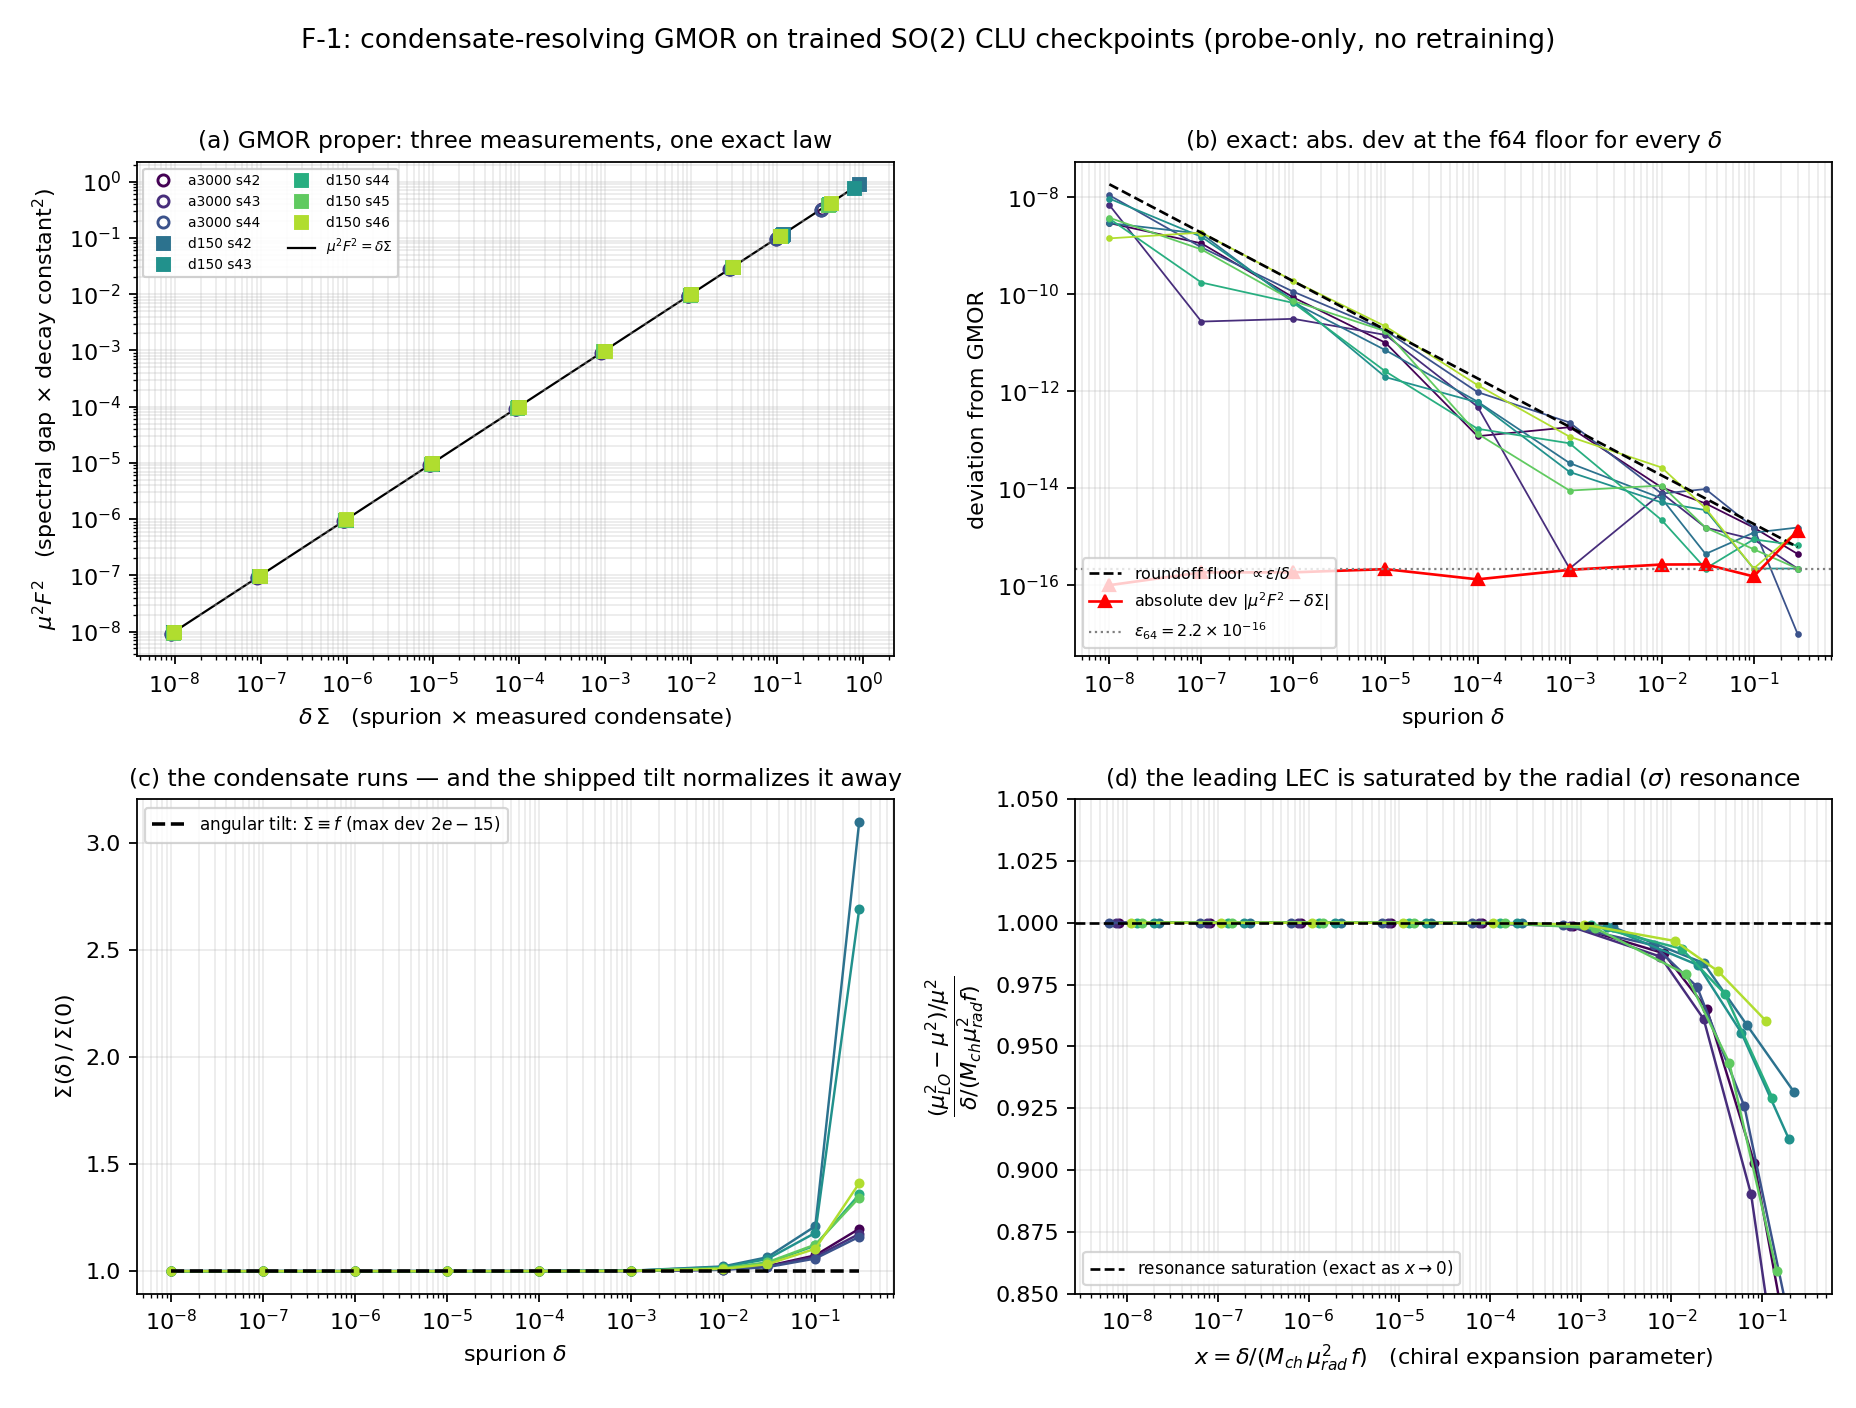
\includegraphics[width=\textwidth]{figs/fig_gmor_condensate.png}
\caption{GMOR proper on trained checkpoints, with a linear ambient spurion. (a) The collapse $\mu^2F^2=\delta\Sigma$ over $8$ decades of $\delta$, $8$ trained $SO(2)$ checkpoints. (b) Absolute deviation pinned at the $f64$ floor ($\le1.33{\times}10^{-15}$) against the $\epsilon/\delta$ relative-roundoff line of the autodiff Hessian --- the small-$\delta$ relative residual is a probe artifact, not a law violation. (c) The running condensate $\Sigma(\delta)/\Sigma(0)$ under the linear spurion versus the angular tilt's exactly flat $\Sigma\equiv r^*$ --- the shipped tilt cannot see the condensate. (d) The LEC ratio $\to1$ as the chiral expansion parameter $x\to0$, slope $-1.05$. \emph{(Designed testbed, analytic spurion, trained checkpoints $\Rightarrow$ verification.)}}
\label{fig:gmor}
\end{figure}

\section{The $T=0$ face of the budget cube: finite-temperature coset diffusion, designed and emergent}\label{app:tcube}
\emph{(Sources: \texttt{t-lever-forgetting}, $5$ trained designed-$SO(2)$ checkpoints, $f64$ probes --- \textbf{designed testbed $\Rightarrow$ verification}; and \texttt{v5-gate}, $3$ trained emergent-MLP checkpoints $+$ a matched designed control, $f64$ probes --- \textbf{learned system $\Rightarrow$ evidence}. Provenance: B.7, B.8. \textbf{Placement note:} this appendix discharges the Coleman/Mermin--Wagner obligation of \S2 and is retained in full per our appendix policy; whether it ships here or in a longer separate treatment is a pending editorial decision.)}

\emph{\textbf{Mandatory flag, travels with every number in this appendix.}} All results require \texttt{langevin\_noise="fdt"} --- the fluctuation--dissipation-consistent noise scale $\sigma^\star_i=\sqrt{M_iT\gamma(2-\gamma)}$ --- \textbf{and a Newtonian kinetic mode} (\texttt{newtonian\_identity}/\texttt{newtonian\_learned}). The reference implementation's \textbf{default is \texttt{legacy}}, under which $T$ is not in energy units and \textbf{none} of these laws hold; and in the relativistic kinetic mode no noise scale targets Gibbs at all (Appendix~G; theory note, Prop-9$'$), so the laws are undefined there. The checkpoints here are \texttt{newtonian\_learned} (B.7/B.8), so every number below is in scope. Nothing in \S3 depends on this appendix: all main-text retention results are $T=0$ deterministic rollouts.

\textbf{The split, stated first (what generalizes and what does not; lead with the general result).} Two of the three faces below are architecture-general; one is not. \textbf{(b) The damping-optimum unification and the $T>0$ diffusion law generalize to the learned (MLP) arm} (evidence, $3$ emergent seeds): the emergent coset half-life $n_{1/2}(\gamma)$ is the \emph{same} non-monotone V-curve, and the friction-lengthens-memory sign flip replicates in $10/10$ conditions above a measured crossover $T^\star\approx3{\times}10^{-3}$ (K.4). \textbf{(a) The latch \emph{register} is designed-only} (evidence for the negative, $3$ emergent seeds, N46): an emergent unit has no continuous coset register --- it stores $\approx1$--$1.6$ bits on $2$--$3$ discrete washboard minima, not a real-valued angle (K.1). So \emph{one damping-optimum curve governs retention across eleven orders of magnitude in $\mu^2$, but the register it operates on is an architectural object you must design in.} \textbf{Instrument warning (travels with every exponent below).} Raw $\mathrm{d}\log n_{1/2}/\mathrm{d}\log T$ and $\mathrm{d}\log n_{1/2}/\mathrm{d}\log\gamma$ exponents are \textbf{not} discriminating designed-vs-emergent: a matched designed control on the same $(\gamma,T)$ grid gives the \emph{same} shallow slopes, because both carry the $\ell_\theta/\Delta$ boundary-layer bias of K.5 (K.6). \textbf{Never quote an $n_{1/2}$ without its $\Delta$ and $\ell_\theta/\Delta$.}

\textbf{K.1 Friction cannot erase a Goldstone register --- on the \emph{designed} arm (an operator identity, on trained weights; verification).} The flat-mode multiplier satisfies $\big||\lambda_{\rm flat}|-1\big|\le1.7{\times}10^{-14}$ at \textbf{every} $\gamma\in[0.002,0.5]$ ($22$-point geometric grid, $5$ seeds; $f64$ eps $=2.2{\times}10^{-16}$), and latch drift is $\le4.9{\times}10^{-12}$~rad over $2{\times}10^5$ steps across $30/30$ (seed,$\gamma$) cells. A friction field applied to a flat direction is a \textbf{no-op on stored content}: it drains only the momentum of a write in progress.

\textbf{The emergent arm has no such register --- this face is designed-only (evidence; negative N46).} On the trained emergent (MLP) checkpoints the direction of largest coset overlap is \textbf{not} flat and barely soft: a middle-of-spectrum massive mode only $1.7$--$4.9\times$ softer than the \emph{stiffest} mode in the whole Hessian spectrum, with $1-|\lambda_{\rm coset}|\approx10^{-3}$ at $\gamma\approx0.05$ (min $\approx8{\times}10^{-5}$ over the $\gamma$-grid) versus the designed $\le1.1{\times}10^{-15}$ --- a $\sim\!12$-order-of-magnitude gap. Consequently a written coset value $\delta\in\{0.1,0.3,0.5\}$~rad \textbf{relaxes completely} back to the nearest washboard minimum ($|{\rm retained}|\le2.1{\times}10^{-3}$, $3$ emergent seeds, $T=0$), where the designed unit retains $\delta$ exactly. \textbf{An emergent unit therefore stores nothing on a continuum:} its coset ``register'' has capacity $\approx\log_2(2\text{--}3\ \text{minima})\approx1$--$1.6$ bits. This is the sharp form of \S3.4's designed-vs-emergent gap, logged as negative N46 (Appendix~G).

\textbf{K.2 The coset diffusion law.} At $T>0$ the coset coordinate is an unbiased random walk with $D_\theta=\varepsilon T(2-\gamma)/(2F^2\gamma)$, $F^2=M_{\rm ch}r^{*2}$, verified to $\hat D_\theta/D_\theta^{\rm pred}=1.0068\pm0.0219$ over $25$ $(\gamma,T)$ cells (min $0.9644$, max $1.0484$), with $\mathrm{d}\log D/\mathrm{d}\log T=+0.992\ldots+1.010$ and, after dividing out the discrete $(2-\gamma)$ factor, $\mathrm{d}\log D/\mathrm{d}\log\gamma=-0.980\ldots-1.014$.

\textbf{K.3 The sign flip: friction remembers, temperature forgets.} $\partial n_{1/2}/\partial\gamma>0$ on $10/10$ (seed,$T$) conditions: $\mathrm{d}\log n_{1/2}/\mathrm{d}\log\gamma=+0.955\pm0.042$ ($T{=}10^{-3}$, $5$ seeds), and $\gamma{:}\,0.05\to0.2$ \textbf{lengthens} the coset half-life by $3.77\pm0.23\times$ (per-seed $3.55/3.64/3.61/3.89/4.15$). In $T$: $\mathrm{d}\log n_{1/2}/\mathrm{d}\log T=-0.956\ldots-0.979$. Absolute law $n_{1/2}(\text{median})=0.378748\,\Delta^2F^2\gamma/(\varepsilon^2T(2-\gamma))$, verified to $1.054\pm0.057$ once $\ell_\theta/\Delta<0.05$.

\textbf{K.4 Unification with the budget's damping corollary (Appendix~F.2) (supersedes any ``two laws'' reading).} The \emph{massive} mode's $n_{1/2}(\gamma)$ is \textbf{non-monotone}, with a minimum at critical damping $\gamma_{\rm crit}=2\varepsilon\mu$: slope $-1.006$ below, $+1.23$ to $+1.27$ above. The flat mode is exactly the $\mu\to0$ corner where $\gamma_{\rm crit}\to0$, so a coset is \textbf{permanently overdamped} --- which is \emph{why} its $\gamma$-dependence has the opposite sign to the massive mode's. \textbf{One damping-optimum curve evaluated at two values of $\mu$, not two laws} --- the same $\gamma^*\approx2\varepsilon\mu$ minimum verified in \S3.1.

\textbf{This unification is an emergent-arm result, not a designed-only one --- the general face of the appendix (evidence, $3$ MLP seeds).} On the trained emergent checkpoints the $T=0$ half-life $n_{1/2}(\gamma)$ (coset-tracked Jacobian eigenvalue) is the \emph{same} V-curve: minimum at $\gamma_{\rm crit}=2\varepsilon\mu_{\rm soft}$, measured $\mathrm{argmin}_\gamma/\gamma_{\rm crit}=0.902\pm0.003$ ($3/3$ seeds; the $10\%$ deficit is the known discrete-map correction), slope $-1.0020\pm0.0003$ below and $+1.116\pm0.011$ above. The designed coset is the $\mu\to0$ corner of \emph{this very curve} ($n_{1/2}=\infty$ at all $\gamma$), so one curve now spans \textbf{eleven orders of magnitude in $\mu^2$} ($1.7{\times}10^{-12}$ designed $\to7{\times}10^{-2}$ emergent). \emph{(Instrument note, so the spans quoted in this paper cannot be read as inconsistent: the designed endpoint here is the smallest $\mu^2$ the \textbf{Jacobian-derived} $\gamma$-grid probe of B.8 can resolve on this curve --- not the \textbf{Hessian} $\mu^2\le2.4{\times}10^{-15}$ of \S3.3/B.1, which is the number in the $13$--$14$-order designed-vs-emergent protection gap. Different instruments, same architectures: eleven orders is the span of one measured curve, $13$--$14$ orders is the Hessian gap between the two vacua.)} The $T>0$ face likewise generalizes: $\partial n_{1/2}/\partial\gamma>0$ in $10/10$ emergent (seed,$T$) conditions ($\Delta=0.5$~rad; B.8) above a measured crossover $T^\star\approx3{\times}10^{-3}$ (predicted $2.7$--$3.7{\times}10^{-3}$), below the washboard barrier ($2.3$--$3.6{\times}10^{-2}$); above $T^\star$ the emergent coset obeys the exact-Goldstone diffusion law to $\pm25\%$, while below it the pseudo-Goldstone mass \emph{protects} the register (sign positive in both channels). \emph{Two observables, two signs:} the register written \textbf{off} the vacuum carries this V-curve's $-1.0020$ slope on its $\gamma<\gamma_{\rm crit}$ branch --- always name the initial condition. \textbf{The raw $T$- and $\gamma$-exponents on this grid are \emph{not} discriminating designed-vs-emergent (K.6); only bias-corrected deep-diffusive cells support a physics claim.}

\textbf{K.5 A new qualifier: the thermal persistence length.} The law requires $\Delta\gg\ell_\theta=\varepsilon\sqrt{T/M_{\rm ch}}/(\gamma r^*)$, the \textbf{thermal persistence length} --- a coset register's physical resolution limit at temperature $T$. Below it the walker is ballistic and $n_{1/2}$ inflates by $\approx(1+\ell_\theta/\Delta)^2$. Controlled against an exact AR(1)-coset toy: $n_{1/2}(\text{trained})/n_{1/2}(\text{toy})=1.0020\pm0.0495$ over $20$ cells --- \emph{the trained coset behaves as the ideal flat coset, cell by cell, to $0.2\pm5.0\%$.}

\textbf{K.6 Honest scope (updated: the emergent arm is now tested).} The designed measurements (K.1--K.5) are on one architecture --- the exact-$SO(2)$ channel, dim $4$, $5$ seeds, laptop-CPU, \texttt{fdt} noise, \texttt{newtonian\_learned}, checkpoints re-tied --- and are labeled verification. The emergent generalization (K.1's negative; K.4's V-curve and $T^\star$) is on $3$ MLP checkpoints of the same configuration and is labeled evidence. \textbf{Designed-only:} the continuous latch register (N46). \textbf{Generalizes:} the damping-optimum unification and the $T>0$ diffusion law (above $T^\star$). \textbf{Instrument caveat (load-bearing).} On a matched designed control run at the same $(\gamma,T)$ grid the raw exponents are $\mathrm{d}\log n_{1/2}/\mathrm{d}\log T=-0.53,-0.60,-1.04$ and $\mathrm{d}\log n_{1/2}/\mathrm{d}\log\gamma=+0.78,+0.63,+0.55$ --- \textbf{indistinguishable from the emergent values} --- because both families carry the $\ell_\theta/\Delta$ boundary layer ($\ell_\theta/\Delta$ up to $2.0$ on this grid, which reaches $T=3.2{\times}10^{-2}$ and $\gamma=0.01$). No emergent-vs-designed claim may be read off raw exponents; the sign-flip finding rests on the $10/10$ \emph{sign} and on the bias-corrected deep-diffusive ($\ell_\theta/\Delta<0.06$) cells. Linear response still requires $T\le3{\times}10^{-3}$; the $T{=}10^{-2}$ column of every designed sweep is anharmonic (equipartition ratio $1.047$--$1.112$) and its exponents are not quoted. Raw designed half-life ratios ($1.257\pm0.261$) must never be quoted without the $\ell_\theta/\Delta$ boundary-layer correction; the deep-diffusive figure is $1.054\pm0.057$. \textbf{Remaining risks:} three emergent seeds, one $150$-epoch \texttt{newtonian\_learned} MLP configuration, no high-dim and no relativistic kinetic mode; the emergent $T^\star$ straddles two $T$ cells per seed. This appendix supplies the $T$ axis of a $(\mu,\gamma,T)$ budget cube whose $T=0$ face is the table of \S2; the cube itself is horizon, not result (\S5).

\section{Positioning and prior art (full), and four claims we retire}

\emph{(Expository/positioning appendix. It carries, in full, the prior-art discussion compressed into \S4, and it records four positioning claims this paper does \textbf{not} make. No result in this paper depends on this appendix; it exists so that a reviewer's first four objections are answered in writing.)}

\textbf{L.1 ``Attention and state-space models have no retention-guarantee analogue'' --- retired.} They do. HiPPO-LegS (Gu, Dao, Ermon, Rudra \& Ré, NeurIPS 2020) proves an approximation-error bound $O(tL/\sqrt N)$ for its online function approximation and, more pointedly for memory, a \textbf{$\Theta(1/t)$ gradient decay --- polynomial rather than exponential} --- which is exactly the kind of guarantee our $\mu^{-2}$ law provides in a different currency. It also carries a property we cannot match: its timescale-equivariance proposition is \emph{exact} and involves \textbf{no discretization step at all}, whereas every statement in this paper is a statement about a discrete map at a fixed $\varepsilon$, with $h=\varepsilon\mu<2$ as a hard stability limit. \textbf{The honest position, recorded here because a reviewer will ask it:} we have no evidence that a learned inertial-mass spectrum is preferable to provable timescale invariance, and we do not claim it. What we offer instead is a \emph{constitutive} account --- which learned quantity sets a mode's lifetime, to what precision, and where the account breaks (the exceptional point) --- on trained models.

\textbf{L.2 ``Retrieval is a rollout, not a weighted sum'' as our novelty --- retired.} Kong, Brewer \& Lai (\emph{Nature Communications} 15, 2024) demonstrate location-addressable retrieval of \emph{dynamical attractors} via an index channel, with a capacity scaling $N_c\propto K^{1.08\pm0.01}$ (their one-hot and binary index codings; $1.17\pm0.02$ for their 2D coding). The move --- retrieve by running dynamics from an addressed initial condition rather than by summing stored vectors --- is theirs and must be cited as such. The differences that remain are structural rather than conceptual: their system is not symplectic, not Hamiltonian, not mass-structured, and the address enters through a dedicated index channel rather than as the initial condition of the state. We record the distinction and claim nothing beyond it.

\textbf{L.3 ``Continuity is our escape hatch from the NTM/DNC lineage'' --- false, and retired.} Both the Neural Turing Machine (Graves, Wayne \& Danihelka 2014) and the Differentiable Neural Computer (Graves et al. 2016) were already fully soft, continuous and end-to-end differentiable; the discrete-action variants are a separate later line. The precedent therefore transfers as a \textbf{warning, not as a contrast}. Csordás \& Schmidhuber (ICLR 2019) diagnose three DNC failure modes, and two of them bite any scheme of the kind studied here: \textbf{key/value entanglement} --- which they rank as the most important, and which is \emph{architectural} in a memory whose address $q_0$ is simultaneously the key and the initial condition of the value --- and de-allocation aliasing, which maps onto any position-gated forgetting mechanism. Chained-read degradation is the third. None of these are measured in this paper; naming them is the point of this entry.

\textbf{L.4 ``A competitor to the transformer'' --- never claimed, and indefensible at this scale.} At $\approx1$--$1.6$ bits per emergent register (Appendix K.1, negative N46) and with no win over a trivial baseline on any external benchmark, a capability claim against attention would be unserious. Benchmarks in this area enforce parameter matching for a reason, and there are formal results on the limits of fixed-size latent state for copying and retrieval (Jelassi et al., ICML 2024) that symplectic conservation does not evade --- conservation prevents \emph{decay}, not \emph{capacity}. Even the strongest recent recurrent architectures claim to advance a performance--efficiency frontier rather than to replace attention. \textbf{Approved positioning, and the one used in \S4:} a physics-structured associative memory in which retention is a designed, per-item property --- permanent (symmetry-protected) or of a finite, $\mu^2$-set half-life --- rather than an emergent consequence of a learned recurrence. This claims controllability, which we evidence; not capability, which we do not.

\textbf{L.5 What \emph{does} survive, and the neighbours that bound it.} Three positive positioning statements are defensible on the evidence in this paper. \textbf{(i)} Energy-landscape retrieval and attention are not analogues but the same object in a precise sense --- the modern Hopfield update \emph{coincides with} the attention mechanism (Ramsauer et al., ICLR 2021 --- exactly so for a single head with identity projections and $\beta=1/\sqrt D$) --- so a landscape-based memory competes on principled ground rather than by metaphor. \textbf{(ii)} Permanence as a \emph{per-item write-time design parameter} with qualitatively distinct modes, one of them exactly symmetry-protected ($\mu^2\equiv0$ by Sylvester congruence, for any inertia), is narrower than ``tunable memory permanence'' as such, which is occupied (EDEN; Karuvally, Lertsaroj, Sejnowski \& Siegelmann, NeurIPS 2025: analytic escape times, a static/dynamic phase transition, capacity $O(\gamma^N)$). \textbf{(iii)} The structure-preserving half of the story is bounded by \textbf{UnICORNN} (Rusch \& Mishra 2021b, ICML), an explicitly Hamiltonian, structure-preserving (symplectic) recurrent unit that comes with a gradient-bound theorem we do not have --- so ``symplectic implies long-horizon stability'' is cited, not claimed, and our own boundedness statements are scoped to the autonomous, designed setting we measure (\S5). The nearest published neighbour to this paper's \emph{write} is test-time gradient descent with momentum on an associative-memory loss (Titans; Behrouz, Zhong \& Mirrokni, NeurIPS 2025), which is a discretized damped second-order dynamics of the same family; the difference we can point to is that our damping and inertia are \emph{read out and priced} ($\gamma$, $M$, $\mu$) rather than chosen as optimizer hyperparameters.

\textbf{L.6 Scope of this appendix.} It is a positioning record, not a survey: it covers the claims a reviewer of \emph{this} paper is most likely to test, and every retirement above is a claim we have deliberately removed from our own writing rather than a criticism of the cited work.

\section{The long-form main text, retained in full}\label{app:longform}
\emph{This appendix is the \textbf{unabridged} version of \S1--\S5, retained verbatim under our appendix policy: the main text is written to the venue's 4-page budget, and nothing that budget displaced has been cut. Section titles below are the long-form's own and correspond one-to-one to the main text's sections; every number carries the same flag-provenance rows (Appendix~B) as its main-text counterpart. Figures 2b and 3, displaced from the main text by the page budget, are displayed here. \textbf{Notation:} this long form writes the unbroken subgroup as $H$, as the sources it reproduces do, where the condensed main text and Appendix~A write $\mathcal H$ for the same object; the Hamiltonian $H(q,p)=T(p)+V_\theta(q)$ is always written with its arguments.}

\subsection*{M\S1. Introduction}

Recurrent memory is usually engineered by fighting the exploding/vanishing-gradient tradeoff with gates. A parallel line replaces the black-box gated update with a \textbf{structure-preserving physical integrator}: a latent state $(q,p)$ is advanced by a symplectic (leapfrog / velocity-Verlet) step of a learnable separable Hamiltonian $H(q,p)=T(p)+V_\theta(q)$, with an optional per-step momentum damping $p\mapsto(1-\gamma)p$ supplying controllable forgetting. This paper is about \textbf{what memory in such a \emph{trained} network obeys} --- not a new architecture, but a closed-form account of retention that we verify on trained models and contrast, head to head, with both a published machine-learning lifetime law and well-trained recurrent baselines.

Our reference unit is the \textbf{CLU (Causal Learning Unit), introduced as CHLU in Jawahar \& Pierini (2026)}; every result below is stated for the class of damped symplectic recurrences and, except where noted, uses no property specific to the reference training objective. The exactly-solvable theory we verify is developed in a separate note (Anonymous, 2026; hereafter \emph{the theory note}); this paper is its evidence-side counterpart, phrased for a machine-learning reader.

\textbf{Nomenclature (used throughout, do not conflate).} Two quantities both get called ``mass'' and run in opposite directions: the \textbf{inertial mass} $M_i$ (the learned diagonal of $T$; larger $M$ $\Rightarrow$ slower) and the \textbf{spectral mass} $\mu_k$ (normal-mode frequency $\mu_k^2=\lambda_k(M^{-1/2}\nabla^2V_\theta M^{-1/2})$ at a critical point; larger $\mu$ $\Rightarrow$ shorter memory). All retention statements use $\mu$.

\textbf{Framing: two axes, not one.} It is tempting to read ``latched / overdamped / underdamped'' as three modes of one classification. They are two axes. \textbf{Axis 1, the symmetry realization} of the trained potential $V_\theta$ at its vacuum, fixes each mode's spectral mass $\mu^2$ --- a statement about the potential and its symmetry alone, with no reference to the integrator. \textbf{Axis 2, the map's regime} $(\varepsilon,\gamma,T)$, decides what a given $\mu^2$ buys: an infinite-lifetime latch, an overdamped register with a $\mu^{-2}$ half-life, an underdamped working memory at the mass-independent floor, or (at $T>0$) a diffusive register. The mode-mass budget that occupies most of this paper is the \emph{axis-2} law, and it is what we measure; the realization taxonomy is the \emph{axis-1} law, and it is what organizes the results. We make the axis-1 statement precise in \S2.1, where it also pays for itself: all three realizations are exhibited by trained models in this paper, and the one the literature would call a training pathology (\S3.5) is exactly the unbroken (Wigner--Weyl) cell.

\textbf{Contributions.}
1. \textbf{The mode-mass budget, verified on trained models (\S3.1).} On trained units the GMOR retention law $n_{1/2}\propto\mu^{-2}$ holds to a fitted overdamped slope $-0.985$ (predicted $-1$), the spectral-mass identity $\mu^2_{\mathrm{meas}}/\mu^2_{\mathrm{pred}}=1.000000\pm5\!\times\!10^{-12}$ over $4.5$ decades, saturation at the mass-independent floor $2\ln2/(-\ln(1-\gamma))$, and the exceptional-point $\sqrt{h-h^*}$ frequency onset with its measured retention-metric bifurcation ($5$ designed seeds, dim $4$, laptop-CPU). \emph{(Designed testbed, analytic tilts $\Rightarrow$ labeled verification.)}
2. \textbf{Mo head-to-head on trained models (\S3.2, headline).} A published single-exponential lifetime law is the \emph{overdamped face} of the budget: measured/predicted ratio $1.012$--$1.029$ overdamped (its published median $1.013$), $2.20\pm0.16$ at the exceptional point, collapsing to $0.31\pm0.01$ deep underdamped --- reproduced on Mo's \emph{own} finite-horizon estimator, not only on a substituted predictor.
3. \textbf{GMOR proper on trained checkpoints (\S3.1, Appendix J).} A condensate-resolving \emph{linear} spurion upgrades the shipped angular tilt's power law to the full Gell-Mann--Oakes--Renner identity $\mu^2F^2=\delta\Sigma$, to $1.33\!\times\!10^{-15}$ absolute with all three objects measured independently on $8$ trained $SO(2)$ checkpoints, and exhibits resonance saturation of the leading low-energy constant by the radial mode (ratio $\to0.99999607$). \emph{(Designed testbed, analytic spurion $\Rightarrow$ verification.)}
4. \textbf{The symmetry-realization taxonomy, exhibited by trained models (\S2.1).} Axis 1 --- the realization of the trained potential's symmetry at its vacuum --- has exactly three cells, and each is realized by a trained model in this paper: unbroken (the contrastive-divergence--eroded vacuum, \S3.5), spontaneously broken (the designed $SO(2)$ unit), explicitly broken (analytic tilts; the self-broken MLP). The taxonomy is what makes ``latched / overdamped / underdamped'' two axes rather than one classification, and it names as a \emph{symmetry restoration} what the literature would call a training pathology.
5. \textbf{Designed vs. emergent, and the price of physics (\S3.4).} Designed symmetry protection beats emergent protection by $13$--$14$ orders of magnitude in $\mu^2$; the physics prior costs raw fit (a param-matched free twin fits $\approx15\times$ better), a cost we localize as contraction-forbidden by volume conservation and whose loan is called at a measured $\approx700$-step crossing. A kinetically-broken battery supplies a measured counterexample showing that map equivariance is \emph{sufficient but not necessary} for a neutral memory direction (\S3.4, \S4).
6. \textbf{Learned-baselines collapse (\S3.3).} On an identical autonomous-retention protocol the structural triad is qualitatively absent in coRNN/LEM/LSTM; a generically-trained unit holds $\approx263$ bounded map-steps and a designed unit latches forever --- with an honest gap (the units cannot enter the input-driven task-RMSE axis, and the map-step ratio inverts under per-step compute normalization; \S3.3, Appendix I).
7. \textbf{Symmetry restoration under training, and the recipe that prevents it (\S3.5).} Wake--sleep contrastive divergence drives the order parameter $r^*$ of a designed degenerate vacuum to zero --- a \textbf{symmetry-restoration (condensate-melting) transition}, not merely a training pathology; a $V(\text{data})$ energy-anchor holds the condensate up across $3000$ erosive epochs, and on those anchored checkpoints ($\approx20\times$ the erosion horizon) every headline law of \S3.1 still holds.

\emph{(A supporting corollary of the budget --- the non-monotone $\gamma$-dependence of the half-life, with its minimum at $\gamma^*\approx2\varepsilon\mu$ --- is reported in Appendix F.2 and is deliberately \textbf{not} a headline of this paper.)}

All experiments are laptop-CPU. Per our reporting discipline, designed-testbed results (architecturally-invariant potentials with analytic tilts or spurions) are labeled \textbf{verification of the theory's exactness}; learned/anharmonic-vacuum results, the training-dynamics results, and the Mo head-to-head are labeled \textbf{evidence}.


\subsection*{M\S2. Setup}

\textbf{The map.} One dissipative velocity-Verlet step with step $\varepsilon$ and per-step damping $\gamma\in[0,1)$ advances $(q,p)$ by a kick--drift--kick of $H=T(p)+V_\theta(q)$ followed by $p\mapsto(1-\gamma)p$. The update is \textbf{conformally symplectic}, $J^\top\Omega J=(1-\gamma)\Omega$ and $\det J=(1-\gamma)^d$, so at each normal mode memory reduces to the eigenstructure of one $2\times2$ matrix (inertia $m$, stiffness $k$, spectral mass $\mu^2=k/m$, dimensionless step $h=\varepsilon\mu$). $\gamma=0$ is exact symplectic leapfrog; $\gamma>0$ appends a uniform momentum contraction. The full derivation, all propositions, and machine-precision checks are in the theory note; we restate only what each result needs.

\textbf{The budget (theory note, \S3--4).} Three bands: a \textbf{latch} ($\mu=0$, symmetry-protected) with frozen displacement $q_\infty=q_0+\varepsilon p_0/(M\gamma)$ and infinite half-life; an \textbf{overdamped register} ($0<\varepsilon\mu\lesssim\gamma/2$) with $n_{1/2}\approx\tfrac{2\gamma\ln2}{(2-\gamma)(\varepsilon\mu)^2}$; and an \textbf{underdamped working memory} ($\gamma/2\lesssim\varepsilon\mu<2$) oscillating at $\approx\mu$ with the mass-independent envelope half-life $2\ln2/(-\ln(1-\gamma))$. The over/underdamped boundary is the exceptional point $h^*\approx\gamma/2$. (The budget also implies a non-monotone $n_{1/2}(\gamma)$ with a minimum at $\gamma^*\approx2\varepsilon\mu$; we verify that corollary but report it as a supporting result in Appendix F.2, not as a headline of this paper.)

\textbf{Trained models.} Unless noted, the trained checkpoints are the reference unit's Experiment-D configuration (dim $4$, hidden $64$, learned-Newtonian kinetic term, $\mathrm{dt}=0.05$, a unit circle $R=1$ sampled at $256$ points), trained at $150$ epochs (see \S3.5 / Appendix C for why $150$ and not the default $1000$). Two potential families: \textbf{designed} = an architecturally-$SO(2)$-invariant $V_\theta$ (\texttt{so2\_invariant}, $5$ seeds), and \textbf{emergent} = a generic MLP $V_\theta$ trained on the same symmetric data ($3$ seeds). Full flag-provenance in Appendix B.

\subsubsection*{M\S2.1 Symmetry realization: the axis that sets $\mu^2$}

\emph{(Readers without a field-theory background may prefer to read Appendix A first: a self-contained $SO(2)$ symmetry-breaking primer, written for a machine-learning audience. It is expository and defers to the definitions of this subsection, which are the ones this paper uses.)}

Axis 1 has exactly three cells, and each is realized by trained models in this paper:

\begin{center}\small
\begin{tabular}{@{}p{1.55in} p{1.15in} p{1.85in} p{1.5in}@{}}
\toprule
realization & vacuum $q^*$ & spectral mass $\mu^2$ & realized by (this paper) \\
\midrule
\textbf{Wigner--Weyl} (unbroken) & $G$-invariant ($r^*=0$) & $\mu^2>0$, \textbf{degenerate within each irrep} (Schur) & the contrastive-divergence--eroded vacuum (\S3.5) \\
\textbf{Nambu--Goldstone} (spontaneously broken) & on a $G$-orbit ($r^*>0$) & $\mu^2=0$ \textbf{exactly}, along $\dim(G/H)$ directions & the designed $SO(2)$ unit (\S3.1, \S3.3) \\
\textbf{pseudo-Goldstone} (explicitly broken) & tilted orbit & $\mu^2=\delta\Sigma/F^2>0$, small & analytic tilts (\S3.1); the self-broken MLP (\S3.4) \\
\bottomrule
\end{tabular}
\end{center}

\textbf{Scope of the explicitly-broken cell, stated where the cell is introduced.} Every explicit breaking in this paper is either an \emph{analytic} tilt or spurion applied to a designed, architecturally-invariant potential (\S3.1, Appendix J) or the \emph{self}-breaking that a generic MLP potential develops on symmetric data (\S3.4). The \emph{tilt-as-a-lifetime-dial} construction is therefore claimed for \textbf{designed geometries only}; the MLP's self-breaking is an \emph{observed} instance of the cell, budget-priced in \S3.4, not a dial we set. In a separate battery of ours on a \emph{learned}, multi-atom store --- a different architecture, in which an explicit-breaking coefficient was intended as the register's lifetime dial --- the effect ran the other way: the softest eigenvalue decreased monotonically as the breaking coefficient was raised, and a coercive confinement term, not the breaking, set the achievable lifetime ceiling. That negative is recorded in full in Appendix G (N149/N150), and it fences the results below: nothing in this paper licenses reading an explicit-breaking coefficient as a lifetime dial on a learned store.

\textbf{What ``spontaneous symmetry breaking'' means for a finite-dimensional deterministic system.} We use only the \emph{classical, tree-level} Goldstone theorem, which is a statement about a Hessian and not about a thermodynamic limit: if $V_\theta$ is $G$-invariant and its minimiser $q^*$ is \textbf{not} $G$-invariant, then the whole orbit through $q^*$ consists of minimisers, and $\nabla^2V_\theta(q^*)$ annihilates every orbit tangent --- exactly $\dim(G/H)$ zero eigenvalues. Nothing in this requires a large system, a phase transition, a thermodynamic limit, or $\hbar$. Throughout, ``spontaneously broken'' means precisely \emph{the minimiser is not $G$-invariant}, and ``Goldstone mode'' means precisely \emph{zero Hessian eigenvalue along the orbit}. That is exact for the dim-$4$ units we train, and it is the only sense in which we use the words.

\textbf{Coleman / Mermin--Wagner, stated honestly.} A continuous symmetry cannot be spontaneously broken in a $0{+}1$-dimensional \emph{thermal} system, and our latch does not contradict this: \textbf{the infinite half-life is a $T=0$ statement} about the deterministic damped map. At $T>0$ --- i.e. under the Langevin sampler --- the coset coordinate performs a random walk with diffusion constant $D_\theta=\varepsilon T(2-\gamma)/(2F^2\gamma)$, where $F^2=M_{\rm ch}r^{*2}$; the register therefore has a finite, computable lifetime $n_{1/2}\propto F^2\gamma/(\varepsilon^2T)$ and is a \emph{diffusive register}, not long-range order. We verify this law on the trained designed $SO(2)$ checkpoints (dim $4$, $5$ seeds, laptop-CPU, $f64$ probe; Appendix K), where it carries a counter-intuitive corollary --- because $D_\theta\propto1/\gamma$, \textbf{raising friction lengthens coset memory} ($3.77\pm0.23\times$ for $\gamma:0.05\to0.2$, $5/5$ seeds). \emph{Fine print, next to the claim:} this holds only under the fluctuation--dissipation-consistent noise scale $\sigma^\star_i=\sqrt{M_iT\gamma(2-\gamma)}$ \textbf{and a Newtonian kinetic mode} (the trained units here are \texttt{newtonian\_learned}; in the relativistic kinetic mode no noise scale targets Gibbs at all --- Appendix G, theory note Prop-9′); under the reference implementation's legacy noise convention $T$ is not in energy units and none of these $T>0$ laws hold. All main-text retention results in \S3 are $T=0$ (deterministic) and are unaffected.

\textbf{Symmetry protects the \emph{current}; flatness protects the \emph{register}.} The zero eigenvalue above is a property of $V_\theta$ alone. Because congruence by any invertible inertia $M$ preserves the rank and inertia of the Hessian (Sylvester's law; \emph{theory note}, kinetic-spurion blindness), a flat direction keeps $\mu^2=0$ for \textbf{any} inertial anisotropy: the latch is a \textbf{modulus} of $V_\theta$, not a Goldstone mode of the full $H=T+V_\theta$. Kinetic symmetry breaking is invisible to the Hessian and to the latch and appears only in the Noether charge --- the write current. Equivariance of the full map is therefore \emph{sufficient but not necessary} for a neutral memory direction; we substantiate this with a measured counterexample (\S3.4, Appendix D) and cash it against the nearest related work (\S4).

\textbf{What we do not import (honest scope of the correspondence).} The GMOR law of \S3.1 and the ChPT dictionary of Appendix J are \textbf{tree-level and classical throughout}. The unit is $0{+}1$-dimensional classical mechanics: there is no $\hbar$, no field-theoretic propagator, and no fermion content, so there are \textbf{no loops, no chiral logarithms, no running low-energy constants, and no anomaly or Wess--Zumino--Witten structure}, and we make no claim involving any of them. The only expansions used anywhere in this paper are $\varepsilon^2$ (discretization), $T$ (thermal, Appendix K), and the ratio $\mu^2/\mu_{\rm rad}^2$ of pseudo-Goldstone to radial spectral mass (Appendix J). We say this explicitly because a law named after Gell-Mann, Oakes and Renner invites over-reading.


\subsection*{M\S3. Results}

\emph{Reading order (evidence-first). The load-bearing results of this paper are the two that live on trained and learned systems: the \textbf{Mo head-to-head on trained checkpoints} (\S3.2, the headline --- a published ML lifetime law is the overdamped face of the budget) and the \textbf{learned-baselines collapse} (\S3.3 --- the structural retention triad is qualitatively absent in well-trained LSTM/LEM). \S3.1 comes first only because it establishes, to machine precision, that the exactly-solvable $2\times2$ theory \textbf{is} the trained map's angular block --- a \textbf{verification} that licenses reading \S3.2--\S3.4 as evidence about what a trained memory obeys, not as a fit to a designed testbed.}

\subsubsection*{M\S3.1 The mode-mass budget, verified on trained models}

\emph{(Designed testbed, analytic $\cos$ tilts $\Rightarrow$ verification of the theory's exactness. Source: \texttt{v2-full-runs} items 1/3/7, $5$ seeds, dim $4$, laptop-CPU.)}

On the trained designed vacuum (baseline flat-mode $\mu^2=1.2\!\times\!10^{-16}$--$2.4\!\times\!10^{-15}$, machine-flat; channel inertial mass $M_{\rm ch}=0.660$--$0.688$; $r^*=0.959$--$0.991$ across $5$ seeds), we apply analytic symmetry tilts $\delta$ and read off the retention law. The \textbf{constitutive identity is exact}: the Hessian-derived spectral mass equals the measured one-step-Jacobian gap to $3.2\!\times\!10^{-10}$ over all $70$ tilt rows --- the $2\times2$ theory \emph{is} the trained map's angular block. The \textbf{GMOR law holds}: $\mu^2_{\mathrm{meas}}/\mu^2_{\mathrm{pred}}=1.000000\pm5\!\times\!10^{-12}$ at every $\delta$, every seed, across $4.5$ decades, and the overdamped retention power law has fitted slope $-0.985$ ($\delta\le0.06$, $n=35$; predicted $-1$), with absolute agreement $0.7$--$3\%$ deep overdamped. Past the crossover the half-life \textbf{saturates} at the mass-independent floor $27.03$ steps ($=2\ln2/(-\ln0.95)$ at $\gamma=0.05$): the $\delta\ge0.6$ rows straddle it ($38\to31\to25\to31$) within the documented kick-phase ripple.

\textbf{What the angular tilt does and does not measure (nomenclature, and a pointer).} In the ChPT dictionary this experiment measures GMOR in the form $\mu^2F^2=\delta n^2$, where $F^2=M_{\rm ch}r^{*2}$ is the channel's \textbf{decay constant} --- the current--Goldstone coupling defined by $Q=F^2\dot\theta$ on the vacuum orbit. Note that the decay constant is $\sqrt{M_{\rm ch}}\,r^*$, \emph{not} the orbit radius $r^*$; the orbit radius is the \textbf{condensate} $\Sigma=r^*$, the order parameter of \S3.5. The shipped angular tilt $\delta(1-\cos n\theta)$ is radius-independent, so it leaves $\Sigma$ exactly fixed (measured: $|r^*_{\rm tilt}-r^*|\le2.2\!\times\!10^{-15}$) and can only ever measure the \emph{product} $\mu^2F^2$: it is the right instrument for verifying the power law and, provably, the wrong one for resolving $\Sigma$. Appendix J replaces it with a \emph{linear ambient} spurion and measures all three objects independently on the same trained checkpoints, obtaining \textbf{GMOR proper}, $\mu^2F^2=\delta\Sigma$, to $1.33\!\times\!10^{-15}$ absolute ($8$ trained $SO(2)$ checkpoints $\times$ $10$ values of $\delta$, $f64$ probe, probe-only, no retraining).

Two second-order signatures confirm the crossover is a genuine exceptional (defective) point, not a smooth turnover. The \textbf{retention-metric bifurcation} (envelope half-life vs. first-crossing time) is measured: the two agree to $0.01\%$ through the overdamped band and split by up to $3.2\times$ at $\delta=4$ ($31$ vs. $9.8$ steps) --- first-crossing is ballistic ($\propto1/\varepsilon\mu$), envelope is retention; every reported lifetime must name its metric. The \textbf{frequency onset} is $\varphi=0$ exactly below $h^*$ ($15/15$ rows, real eigenvalue pair) and $\varphi\propto\sqrt{h-h^*}$ above, fitted slope $0.5165$ (predicted $1/2$) down to $h-h^*=2.6\!\times\!10^{-6}$. Finally the \textbf{latch transport law} $q_\infty=q_0+\varepsilon p_0/(M\gamma)$ --- the write semantics of the $\mu=0$ band --- holds to $\le1\%$ over two decades of $\gamma$ (measured/predicted $0.9899$ at $\gamma=0.005$ --- a $1.25$-rad transport --- rising to $1.0000$ at $\gamma=0.64$), with the written coset angle then frozen to $\le1.2\!\times\!10^{-15}$ rad over $4000$ steps. The budget table of the theory note is thus reproduced, entry by entry, on trained models. \emph{(EP detail: Appendix F.1. The budget's remaining corollary --- the non-monotone $\gamma$-dependence of the half-life, with its minimum at $\gamma^*\approx2\varepsilon\mu$, confirmed on all $5$ seeds --- is reported in Appendix F.2 as a supporting result and is deliberately not a headline of this paper.)}

\begin{figure}[t]\centering

\includegraphics[width=\linewidth]{figs/fig1_gmor.png}
\caption{\textbf{Figure M1.} The GMOR retention law verified on trained models, and the second-order metric bifurcation. Left: $n_{1/2}$ vs. spectral mass $\mu^2$ on a log--log axis over $4.5$ decades --- fitted overdamped slope $-0.985$ (predicted $-1$), saturating at the mass-independent floor $27.03$ steps ($\gamma=0.05$) past the crossover. Right: the two retention metrics (envelope half-life vs. first-crossing time) agree through the overdamped band and split by up to $3.2\times$ underdamped --- the exceptional point's signature. \emph{(Designed testbed, analytic tilts $\Rightarrow$ verification. Displaced from the main text by the page budget.)}}
\end{figure}

\subsubsection*{M\S3.2 Mo head-to-head on trained models (headline)}

\emph{(Evidence-grade, per our reporting discipline: a published ML law compared on trained checkpoints. Source: \texttt{v2-full-runs} item 2; \texttt{mo-deep-read} \S2--4. Headline = Figure 2, displayed in the main text as Figure 1.)}

Mo (2026) proves that an exactly equivariant recurrent \emph{flow} has \textbf{at least} $\dim(G/H)$ zero Lyapunov exponents along the group orbit --- a lower bound, since unrelated zero exponents can arise from time translation, additional symmetries, conservation laws or finite-time numerical effects --- and shows, in controlled-breaking experiments, that a ``pseudo-gap'' acquired by a formerly-protected direction predicts a finite memory lifetime via a single-exponential estimator. That account is the \textbf{kinematics of protection}: it holds for any equivariant flow and is silent on what \emph{sets} the gap. We run Mo's exact code-level lifetime protocol (initial phase $\phi_0=0.35$ rad, threshold $0.2$ rad, his censoring, cap $15000$ steps) \textbf{unchanged} on the $5$ trained models across $14$ breaking magnitudes, and report the measured/predicted ratio (Figure 2 $=$ main-text Figure 1; seed error bars):

\begin{center}\small
\begin{tabular}{@{}lc@{}}
\toprule
regime & measured / predicted \\
\midrule
overdamped ($\delta=10^{-3}$--$10^{-2}$) & $1.012\pm0.000\to1.029\pm0.001$ (Mo's published median: $1.013$) \\
approaching the EP ($\delta=0.06$--$0.1$) & $1.155\pm0.005\to1.313\pm0.018$ \\
at the EP ($\delta=0.17$, $h\approx h^*$) & $2.202\pm0.155$ \\
underdamped ($\delta=0.6\to4$) & $0.938\pm0.019\to0.309\pm0.012$ \\
\bottomrule
\end{tabular}
\end{center}

\textbf{Mo's law is the overdamped face of our budget.} In his regime the two coincide (rank correlation $\mathrm{corr}(\log\mathrm{pred},\log\mathrm{meas})=0.9987$ overdamped-only; his reported median $1.013$ reproduced), and his single-exponential predictor fails only past the crossover --- by $\approx3.2\times$ at the deepest trained-model breaking we test (measured/predicted $0.309\pm0.012$ at $\delta=4$; our $14$-$\delta$ sweep goes no deeper on the underdamped side), in the calculable ballistic direction, with the EP delay spike ($2.2\times$) as the third signature. The failure mechanism is the retention-metric bifurcation verified in \S3.1, so it does not stop at our deepest trained tilt: on the \emph{exact analytic map} the same single-exponential predictor continues to $\approx5\times$ further underdamped (theory note, Prop. metric-bifurcation and check (k), at $\gamma=0.1$ --- a different damping and a deeper tilt than any trained run here). \textbf{The $\approx3.2\times$ is the trained-model number; the $\approx5\times$ is exact-map only, and we never quote it as evidence about a trained network.} This is a \textbf{containment, not a conflict}: below $h^*$ we recover his published number; above it, the regime structure --- saturation floor, ringing, exceptional point --- is exactly what a first-order flow cannot exhibit and what a \emph{constitutive} (mass-controlled) gap adds. In our damped-Hamiltonian setting the gap is $\mathrm{gap}=\tfrac{(2-\gamma)}{2\gamma}\varepsilon^2\mu^2$ with $\mu^2=\mathrm{eig}(M^{-1}\nabla^2V_\theta)$; Lyapunov analysis, being blind to Jordan/transient structure, cannot see the finite write transport, the $\gamma$-controlled conversion of a drifting integrator into a deadbeat latch, or the Noether charge that acts as the write current (decaying exactly $(1-\gamma)^n$). Where Mo lists conservation laws among \emph{confounding} extra zero exponents, they are our load-bearing structure.

\textbf{Predictor-substitution closed (measured, Figure 2b).} The containment does not depend on substituting the exact Jacobian gap for Mo's own predictor. Re-running the head-to-head with \textbf{Mo's \emph{own} finite-horizon group-tangent estimator $\hat\lambda(T{=}128)$} as the lifetime predictor reproduces the result on his own instrument: overdamped, $\mathrm{corr}(\log\mathrm{pred}_{\hat\lambda},\log\mathrm{meas})=0.9995$ (even tighter than the exact-gap $0.9987$), with measured/predicted $0.86$--$1.03$ bracketing $1$; past the exceptional point the estimator-based prediction fails in the \emph{same} calculable ballistic direction, $0.30$ at $\delta=4$ (mirroring the exact-gap $0.31$). ``Mo's law is the overdamped face'' therefore rests on Mo's actual estimator, not on a substituted predictor. \emph{(Methods caveat, corrected: the finite-horizon $\hat\lambda(T{=}128)$ carries a systematic transient bias vs. the asymptotic gap --- $-15.6\%$ maximum in the deep-overdamped band ($\mathrm{gap}\cdot T<0.1$, transient-dominated at a fixed point), rising to a per-row maximum of $-44.5\%$ that sits at the \textbf{near-EP row} $\delta=0.17$ ($\mathrm{gap}\cdot T\approx3.1$) --- \textbf{not} at $\mathrm{gap}\cdot T\lesssim0.1$ as an earlier draft stated. The prediction curve of Figure 2 uses the exact Jacobian gap; because the rate bias lengthens the }predicted\emph{ lifetime it pulls meas/pred from $1.01$--$1.16$ down to $0.86$--$1.03$, so the lifetime prediction still tracks and the containment claim is robust to it.)}

\emph{(The headline Mo head-to-head figure is displayed in the main text as \textbf{Figure 1}; caption there.)}

\begin{figure}[t]\centering
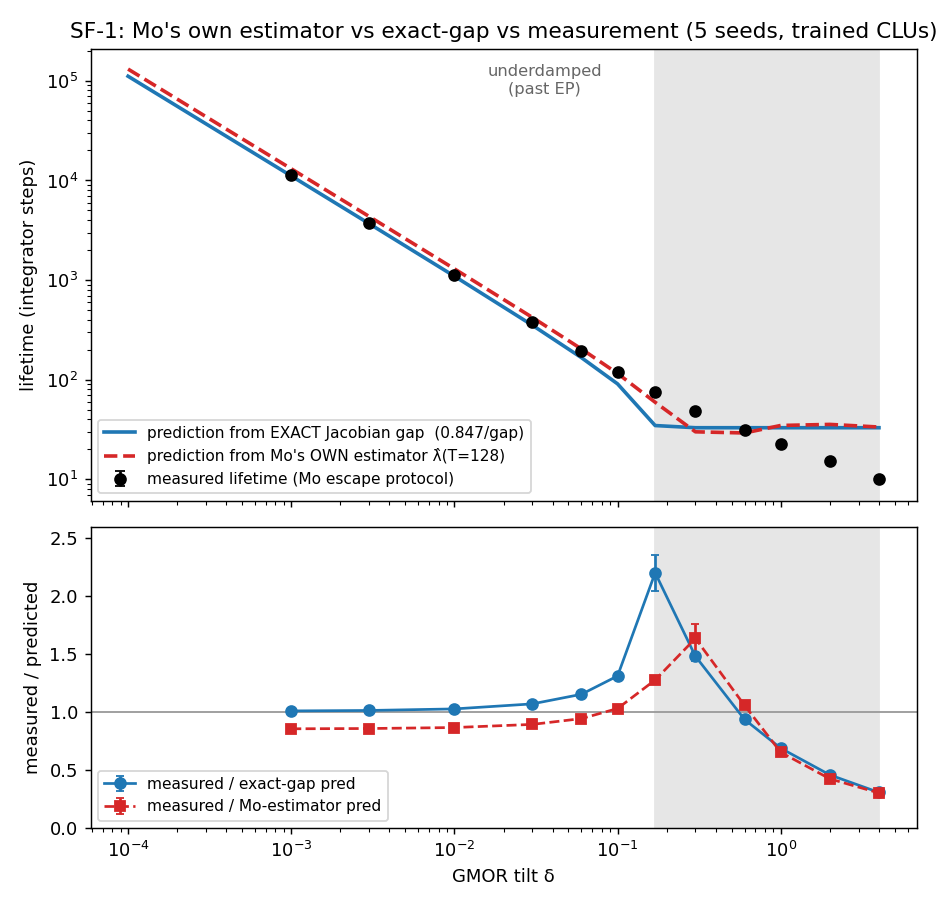
\includegraphics[width=\linewidth]{figs/sf1_mo_estimator_overlay.png}\label{fig:mo_own}
\caption{\textbf{Figure 2b.} Predictor-substitution closed: Mo's \emph{own} finite-horizon estimator $\hat\lambda(T{=}128)$ used as the lifetime predictor (dashed) against the exact Jacobian-gap predictor (solid) and the measured Mo-protocol lifetimes (points), $5$ trained models. Top: all three lifetime curves vs. breaking magnitude $\delta$ (shaded band = past the exceptional point). Bottom: measured/predicted ratio for both predictors --- overdamped both bracket $1$ (Mo-estimator $\mathrm{corr}=0.9995$, meas/pred $0.86$--$1.03$) and both fail identically past the EP ($0.30$ at $\delta=4$). The ``overdamped face'' claim holds on Mo's own estimator, not only on the exact-gap substitute. \emph{(Evidence.)}}
\end{figure}

\subsubsection*{M\S3.3 Learned baselines collapse}

\emph{(Evidence-grade. Source: \texttt{v2-prefreeze-baselines} items 1/2, $5$ baseline seeds, CLU designed $n=5$ / emergent $n=3$, laptop-CPU. Figure 3 = \texttt{figA} retention overlay.)}

We give the trained memory a \emph{learned-architecture} comparison on Mo's $S^1$ path-integration family (input = scalar angular velocity, target = $(\cos\phi,\sin\phi)$). The recurrent baselines are trained with a learning-rate sweep (best-RMSE kept, for fairness) and are \textbf{not strawmen}: LSTM and LEM reach train-horizon (length $64$) RMSE $0.18$/$0.23$ rad ($10$--$13^\circ$); their long-horizon (length $256$) RMSE $0.85$/$0.97$ rad reproduces Mo's own baseline-failure regime. We then run Mo's \emph{autonomous} lifetime protocol --- write a phase, hold with zero input, count recurrent-map applications until the stored phase drifts past $0.2$ rad --- as the \textbf{same observable on every system} (coRNN is a weak entrant at the fixed oscillator hyperparameters $\gamma=\varepsilon=1$, $\mathrm{dt}=0.1$; LSTM/LEM carry the fair comparison, and we do not lean on coRNN).

\begin{center}\small
\begin{tabular}{@{}p{1.5in} p{1.35in} p{1.05in} p{1.05in} p{0.9in}@{}}
\toprule
system & median lifetime (map-steps) & final drift (rad) & perturbed lifetime & budget law? \\
\midrule
coRNN & $5.6\pm1.4$ & $1.55$ (randomized) & $5.1\pm1.0$ & --- (no $\mu^2$) \\
LEM & $56.4\pm19.5$ & $1.66$ (randomized) & $5.0\pm1.1$ & --- \\
LSTM & $68.7\pm18.3$ & $1.28$ (randomized) & $\mathbf{1.8\pm0.8}$ & --- \\
\textbf{CLU-emergent} (generic MLP) & $\mathbf{263}$ ($184$--$436$, $n{=}3$) & $\mathbf{0.35}$ (bounded) & envelope $152$--$812$ & \textbf{yes} ($n_{1/2}$ $152/812/152$ vs. pred $118/687/118$) \\
\textbf{CLU-designed} ($SO(2)$) & $\boldsymbol{\infty}$ (all censored, $5/5$) & $\mathbf{0.00}$ (coset frozen) & $\infty$ & latch ($\mu^2\!\approx\!10^{-15}$) \\
\bottomrule
\end{tabular}
\end{center}

Stated as the approved cross-result finding: \textbf{the structural retention triad --- latch ($\infty$), the $\mu^{-2}$ budget law, and bounded drift --- is qualitatively absent in the learned baselines.} coRNN/LEM/LSTM forget a stored analog phase in $\approx5.6/56/69$ map-steps, their drift randomizes past $1.2$ rad, and their memory is \emph{perturbation-fragile} --- a $0.1$ hidden-state kick collapses the LSTM $69\to2$ and LEM $56\to5$ steps, because a marginally-stable trajectory is not a basin. The generically-trained unit (architecture-matched: a plain MLP potential, no designed symmetry) holds $\approx263$ steps ($\approx4\times$ longer \emph{in map-steps}; per-step compute caveat below), then \emph{saturates} at $\approx0.35$ rad --- it relaxes to the nearest minimum of the self-broken washboard and freezes there (a finite-displacement pseudo-Goldstone, not loss), obeying the budget law to $+12$--$15\%$ at the canonical kick (a per-seed $+5$ to $+29\%$ anharmonic bias; \S3.4/Appendix E). The designed unit never moves (coset angle frozen to $\le10^{-15}$ rad, $5/5$ seeds). This is Mo's neutrality theorem realized exactly: the latch is the mode his kinematics allows but his first-order flows never produce.

\textbf{Honest gap (stated in the main text).} The comparison is on \emph{retention}, in recurrent-map applications --- the fair common unit --- and the load-bearing claim is the \textbf{qualitative triad (latch / $\mu^{-2}$-budget law / bounded drift), which is architecture- and compute-independent}. The raw $263$-vs-$69$-step ratio is a \emph{map-step} statement and \textbf{does not survive compute normalization; we retire it as a compute claim.} Per step, one CLU dissipative-Verlet update (hidden $64$, two $\nabla_qV$ backprops through the potential) costs $\approx6.2\times$ an LSTM cell and $\approx3.1\times$ a LEM cell in wall time ($\approx14$--$15\times$ in FLOPs); normalizing retention by per-step cost, the map-step advantage \textbf{inverts} --- per unit of retention the unit spends $\approx23.5\times$ the wall time of the LSTM it out-holds ($\approx54.8\times$ FLOPs) and $\approx14.6\times$ the LEM ($\approx70.7\times$ FLOPs). \textbf{Confound (must flag):} the comparison is \emph{not} width-matched (CLU hidden $64$ vs. baselines hidden $16$), so a width-matched unit would narrow the gap; the \emph{sign} is robust because the Verlet step requires two potential backprops, and the retention numbers ($263/69/56$) are themselves from these exact configs, so the per-step penalty is the honest apples-to-apples for those results (SF-2; full table Appendix I). On the \emph{input-driven path-integration task-RMSE} axis the RNNs are the only entrants: the unit has no native velocity ingestion, so it cannot compete on Mo's supervised RMSE without an equivariant-control wrapper (a momentum kick along the coset tangent), which is unbuilt. We did not fabricate a task-RMSE for it. This gap is logged as negative N6 (Appendix G).

\begin{figure}[t]\centering
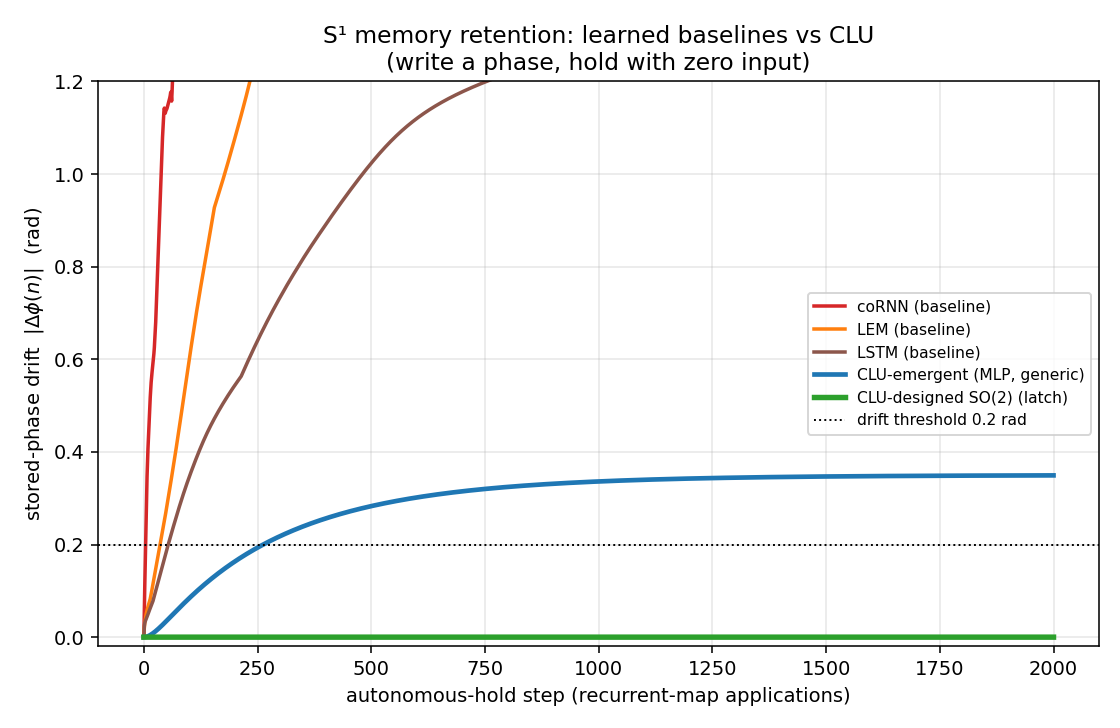
\includegraphics[width=\linewidth]{figs/fig3_retention_overlay.png}
\caption{\textbf{Figure 3.} Autonomous-retention overlay on Mo's $S^1$ protocol (write a phase, hold with zero input, count recurrent-map applications until drift exceeds $0.2$ rad). The learned baselines (coRNN/LEM/LSTM) forget the stored phase in $\approx5.6/56/69$ steps and randomize past $1.2$ rad; the generically-trained unit holds $\approx263$ bounded steps and the symmetry-designed unit latches ($\infty$, coset frozen). The structural retention triad is qualitatively absent in the learned baselines. \emph{(Evidence.)}}
\end{figure}

\subsubsection*{M\S3.4 Designed vs. emergent protection, and the price of the physics}

\emph{(Constitutive-vs-kinematic contrast, foregrounded per our reporting discipline. Sources: \texttt{v2-full-runs} items 4/5 (emergent/isotropization); \texttt{minus-the-physics} Part A (the twin/broken-volume ablation).)}

\textbf{Designed protection beats emergent by $13$--$14$ orders (evidence).} Training a generic MLP potential on perfectly symmetric data develops \emph{no} near-flat direction: the softest emergent spectral mass is $\mu^2=5.1/5.9/5.4\!\times\!10^{-2}$ ($3$ seeds) versus the designed flat mode $|\mu^2|\le2.4\!\times\!10^{-15}$ --- a $13$--$14$ order-of-magnitude gap in memory protection. (The sharp operational form of this gap --- an emergent unit stores nothing on a \emph{continuum}, only $\approx1$--$1.6$ bits on $2$--$3$ washboard minima, while the \emph{damping-optimum retention law itself} still generalizes to the emergent arm --- is Appendix K.1/K.4, negative N46.) The emergent model self-breaks: its potential ripples along the ring at the equivalent of a GMOR tilt $\delta\approx0.01$--$0.06$ (coincidentally inside Mo's breaking grid), pinning discrete angles, whereas the designed model retains all $16/16$ surveyed angles (operational ring degeneracy). Mo's own attribution instrument (equivariance error $E^V_{\rm eq}$) separates the two architectures by $15$ orders ($\approx3\!\times\!10^{-16}$ designed vs. $0.077$--$0.113$ emergent). And the emergent lifetimes are \emph{priced by the budget}, with a small positive anharmonic bias. Under the autonomous protocol at the canonical kick ($0.1$), measured $n_{1/2}=277/257/303$ vs. exact-map (quadratic) prediction $247/227/263$ --- a $+12$--$15\%$ envelope. A \emph{separate} kick-amplitude probe on the \textbf{same three emergent checkpoints} (Appendix E; \texttt{v2-prefreeze-baselines} item 4) extrapolates the per-seed bias to zero kick and resolves it into a \textbf{$+5$ to $+29\%$ spread} (ratios $1.052/1.125/1.288$): a kick-independent settle/discretization offset for $2/3$ seeds and \emph{genuine anharmonicity} on the softest-$\mu^2$ seed, whose retention runs from $\times1.05$ at zero kick up to $\times1.55$ at large amplitude. The bias is therefore \textbf{not uniform across seeds} --- the softest mode is where the quadratic core is loosest --- and its structure is itself predicted by the theory (anharmonicity appears exactly where a soft mode explores a large relative excursion). The two number sets are distinct probes (canonical-kick autonomous protocol vs. kick$\to0$ amplitude sweep) on the same checkpoints, not one decomposing the other.

\textbf{A second falsifiable, answered: no isotropization --- and the register never needed it (evidence, appendix-promoted here for the contrast).} A separate designed battery ($3$ mass-split levels, dim $4$, laptop-CPU) breaks the channel \emph{only kinetically} (untied random-init inertial masses; $V_\theta$ stays exactly invariant by architecture). The learned inertial mass does \textbf{not} self-organize toward isotropy under symmetric data (third independent corroboration): the log-mass split random-walks ($|\log M_0-\log M_1|$: $0.157\to0.155$, $0.037\to0.044$ over $150$ epochs), while tied controls stay at ratio exactly $1.0000$. Crucially the kinetic breaking is \emph{invisible} to the fixed-point Hessian ($\mu^2_{\rm ang}$ stays $\sim10^{-15}$) and to the latch (angular $n_{1/2}=\infty$, write-freeze $=0$ exactly), and \emph{visible only in the charge law}: at $\gamma=0$ the Noether charge undergoes a \textbf{bounded oscillation} --- not a secular drift --- whose amplitude is linear in the split at small split ($5.4/1.6/0.082\!\times\!10^{-2}$ for mass-splits $0.077/0.022/0.0011$; the amplitude-to-split ratio is \emph{not} constant). On the vacuum orbit the exact envelope is $\sqrt{2E}\,r^*(\sqrt{M_{\max}}-\sqrt{M_{\min}})$ with period half a revolution; off the orbit only boundedness holds, $|Q|\le\sup|q|\sup|p|$ by conservation of $H$ on a coercive $V_\theta$.

This is the measured face of a structural fact (\emph{theory note}, kinetic-spurion blindness): congruence by any invertible inertia preserves the Hessian's rank, so \textbf{an anisotropic channel still latches, with infinite half-life}. Three consequences travel with this result. \textbf{(i) The design rule, corrected.} Tie the channel masses to obtain a clean, angle-independent write current --- and, at $\dim(G/H)\ge2$, a degenerate pseudo-Goldstone multiplet --- \textbf{not} to save the register, which was never at risk. \textbf{(ii) Measurement discipline.} To detect kinetic symmetry breaking, measure the charge law; the Hessian and the latch are provably blind to it. \textbf{(iii) A free counterexample.} This battery's map is \emph{not} equivariant (kinetic equivariance error $E^T_{\rm eq}=0.0016$--$0.108$ across the three split levels) and it latches anyway --- so equivariance is sufficient but \textbf{not necessary} for a neutral memory direction (\S4). Symmetry buys the conserved write \emph{current}; the potential's flatness buys the \emph{register}. (Full table: Appendix D.)

\textbf{The price of the physics prior (evidence; scope guard: the cost is contraction-forbidden, and the long-horizon plateau is not claimed).} We build two param-matched controls (dim $4$, $S^1$, $150$ ep, param-matched to $\pm0.05\%$, $3$ seeds, same MLP potential throughout): an \textbf{unconstrained twin} (a free residual recurrence, no Hamiltonian, no volume law) and a \textbf{broken-volume} arm (the same leapfrog and potential plus a learned per-coordinate scaling, bit-identical to the unit at initialization, so only the scaling breaks symplecticity). Running all three through the same measurement harness:

\begin{center}\small
\begin{tabular}{@{}lccc@{}}
\toprule
metric & CLU ($\gamma=0$ conservative) & broken-volume & free twin \\
\midrule
eval MSE (fit; $\downarrow$) & $0.190\pm0.018$ & $0.0785\pm0.004$ & $\mathbf{0.0128\pm0.008}$ \\
BIBO (frac. settled bounded) & $\mathbf{1.00}$ & $0.333\pm0.47$ & $1.00$ \\
flat spectral $\mu^2$ ($\downarrow$ = protected) & $\mathbf{0.008\pm0.015}$ & $0.122$ & --- (no potential) \\
latch coset drift ($\downarrow$ = latches) & $\mathbf{0.19\pm0.19}$ & $0.245$ & $1.15\pm1.2$ \\
vacuum $r^*$ after wake--sleep CD & $\mathbf{0.72}$ (survives) & $\mathbf{0.0}$ (collapsed) & --- (sleep inert) \\
\bottomrule
\end{tabular}
\end{center}

Read as a Pareto statement, not a podium: \textbf{symplectic volume conservation buys bounded (BIBO) dynamics [within the coercive-potential / compact-sublevel-set scope], a protected near-flat memory direction, and vacuum robustness under contrastive-divergence training; the leapfrog structure buys the latch (coset drift $0.19$ vs. twin $1.15$); the physics prior costs raw fit --- the unconstrained twin fits $\approx15\times$ better in MSE.} The measured cost is specifically \emph{contraction-forbidden} by volume conservation (the broken-volume arm recovers $\approx2.4\times$ of the fit precisely by leaking volume), \textbf{not} the causal velocity cap, which is inactive in this arm. Reach-pricing is a second, separately \emph{measured} restriction --- secondary and aggregate-only at single-unit scale ($+77\%$ MSE when the cap binds, collapsing once $v_{\max}\ge$ required speed; \texttt{fit-gap-anatomy} item 1) --- and is deferred to future work at lattice scale.

\textbf{The loan is called at $\approx700$ steps (measured, not asserted).} Tracking cumulative fit vs. horizon on the stationary vacuum (matched params $\pm0.2\%$, $3$ seeds; \texttt{fit-gap-anatomy} item 2, Appendix H): the twin leads by $1$--$2$ orders of magnitude out to $\approx500$ steps, \textbf{crosses above the unit at $\approx700$ steps, and diverges to $196$ at $5000$ steps} --- a free residual recurrence has no bounded-attractor guarantee, so its small per-step residual compounds --- while the unit stays on a bounded plateau $\approx0.20$--$0.23$. The unit's asset is \textbf{boundedness by construction, not the lowest steady MSE}: the broken-volume ($0.14$) and LSTM ($0.13$) arms in fact plateau \emph{below} the unit ($0.22$) --- the physics keeps a small steady-state fit penalty even long-horizon --- but only the unit's boundedness is a \emph{structural} guarantee (the LSTM's is tanh saturation, the broken-volume arm's a learned near-contraction). The twin's $15\times$ edge is a loan, and it is visibly called by $\approx700$ steps.

\textbf{The recovery ladder (which paid mechanism rents back which cheat).} Adding one licensed mechanism at a time to the conservative ($\gamma=0$) unit (\texttt{fit-gap-anatomy} item 3, $3$ seeds; full ladder in Appendix H): \textbf{global damping $\gamma$ recovers $92\%$ of the absolute twin fit gap with BIBO, the latch, and the protected near-flat $\mu^2$ all preserved} --- licensed uniform contraction ($\det J=(1-\gamma)^d$) buys back almost all the fit the twin stole by leaking volume, at zero structural cost. A \textbf{learned friction \emph{field} $\gamma_\phi$ does \emph{not} recover fit ($-24\%$)}: it is a targeted-forgetting tool (there is no trash region to forget on this stationary vacuum), the wrong lever for this gap. The paid mechanisms are \textbf{not interchangeable} --- each rents back a specific cheat and must be matched to it.

\emph{Two comparability caveats, so the ladder is not misread against the table above.} \textbf{(a) Different experiments, different MSE scales.} The Appendix-H ladder is a \textbf{separate wake-only experiment} (\texttt{fit-gap-anatomy}, seeds $\{0,1,2\}$, commit \texttt{9a13455}); its absolute MSE scale and its twin ($0.0047$) are \textbf{not cross-comparable} with the \texttt{minus-the-physics} table above (twin $0.0128$, seeds $\{42,43,44\}$, commit \texttt{b41410f}) --- \textbf{only within-table gaps are meaningful}, and the two tables must never be divided into one another. The $\gamma=0$ conservative rung of the ladder ($0.2066$) is the ladder's own counterpart of the table's $\gamma=0$ CLU ($0.190$), not the same measurement. \textbf{(b) ``$92\%$'' is an absolute-gap fraction, not a ratio.} The $+\gamma$ unit recovers $92\%$ of the \emph{absolute} MSE gap ($0.2066\to0.0216$ against a $0.0047$ twin, gap $0.202$), yet it still \textbf{trails that twin by $\approx4.6\times$ in ratio}. The claim is ``almost all of the absolute contraction-forbidden penalty is licensed back at zero structural cost,'' \textbf{not} ``the unit fits within $8\%$ of a free recurrence.''

\subsubsection*{M\S3.5 Symmetry restoration under training, and the anchored recipe that prevents it}

\emph{(Evidence-grade: a training-dynamics result on learned potentials. Sources: \texttt{v2-full-runs} Finding 0; \texttt{sleep-erosion-study}; \texttt{anchor-robustness}. The positioning of this result against the contrastive-divergence literature, with its coverage statement and chain-length scope clause, is Appendix~C.)}

Read through the axis-1 taxonomy of \S2.1, the result of this section is not a training pathology with an ad-hoc patch: it is a \textbf{symmetry-restoration (condensate-melting) transition} driven by the training objective. The vacuum radius $r^*$ \emph{is} the order parameter $\Sigma$; wake--sleep contrastive divergence drives it to zero, i.e. it moves the trained potential out of the Nambu--Goldstone cell and into the Wigner--Weyl (unbroken) cell, destroying the coset and with it the protected direction the whole construction depends on. The $V(\text{data})$ anchor of the recipe below is precisely what holds the condensate up. \emph{(We use ``restoration'' in the exact classical sense of \S2.1 --- the minimiser becomes $G$-invariant --- and claim no thermodynamic phase transition.)}

The designed vacuum therefore requires a training recipe, because the default one destroys it. At the reference config's default $1000$ epochs, wake--sleep contrastive-divergence training \textbf{inverts} the designed $SO(2)$ vacuum in $8/8$ runs: the ring depth goes $+0.079\to-0.126$ and the order parameter collapses $r^*:1.0\to0$, i.e. the data ring becomes a local \emph{maximum}. The restored phase then displays its own signature, which the taxonomy predicts and which the original report recorded without naming: at the collapsed $G$-invariant vacuum the channel's two spectral masses become \textbf{degenerate} ($\mu^2$ pair $\approx1.0$) --- Schur's lemma at an unbroken vacuum, where there is no orbit, no coset, and hence no protected direction, and the channel modes must fall into one degenerate irrep. The erosion horizon is set by \textbf{sleep-update frequency racing the wake-clamp schedule, independent of chain length}: inversion at epoch $\approx116/442/959$ for sleep frequency $1/5/20$, with the number of sleep sub-steps ($50$ vs. $500$) irrelevant to $\pm1$ epoch and persistence (PCD vs. CD) shifting it $\le9$ epochs. Mechanistically, the initial random negatives' energy shell geometrically overlaps the low-$V$ ring ($22$--$31\%$ in-band early), CD raises $V$ wherever the negatives sit (their mean energy climbs $3.4\to12.3$ monotonically as the ring depth falls), and the ring then expels them. Crucially this is \textbf{specific to flat/degenerate vacua}: a non-degenerate sine vacuum is immune (wake+sleep $\approx$ wake-only), because the wake trajectory-MSE pins $V$'s value at every data point except along a flat coset direction it cannot see.

\textbf{The recipe: anchor $V$'s value at data.} Adding a $V(\text{data})$ energy-anchor term to the wake loss holds the condensate up and cures the erosion cheaply. At $\lambda=10$ the ring depth stays flat at $+0.068$--$+0.072$ over $1000$ epochs with $r^*\approx0.96$, and --- because the sleep phase is retained --- the noise-rejection gap \emph{grows} to $+0.244$, beating even wake-only ($+0.199$). Hardened over a wider envelope (dim $4$, $5$ seeds, $3000$ erosive epochs): $\lambda\in\{1,10,100\}$ all hold the vacuum where $\lambda=0$ always dies, with a strength$\leftrightarrow$robustness tradeoff --- $\lambda=100$ is bulletproof ($5/5$ seeds, $r^*=0.911\pm0.016$) at the cost of weaker noise rejection and $\approx35\times$ higher wake MSE, while $\lambda\approx10$ gives the strongest rejection but leaves $1/5$ seeds able to collapse. The demarcation is \textbf{theory, not a patch}: lifting the flat direction by an explicit tilt $\delta\ge0.05$ immunizes the vacuum with \emph{no anchor at all} (erosion $\propto$ flatness). And the anchor is orthogonal to volume conservation: it does \textbf{not} rescue the broken-volume arm, which diverges under CD regardless --- vacuum survival under CD is a \emph{volume-conservation} payoff, the anchor a separate cure operating only on a bounded symplectic substrate. \textbf{Anchored wake--sleep is the training recipe for the designed unit from here on --- and the paper's headline laws hold under it at $\approx20\times$ the erosion horizon.} Re-verifying the \S3.1 laws on checkpoints trained to $3000$ epochs \emph{with} the $\lambda=100$ anchor ($3$ seeds, $\approx20\times$ past the default-$1000$-ep inversion horizon that destroys the unanchored vacuum): the vacuum is intact (ring depth $+0.10$--$+0.12$, $r^*=0.917\pm0.007$, flat-mode $\mu^2\approx10^{-15}$); the \textbf{GMOR law is still exact}, $\mu^2_{\mathrm{meas}}/\mu^2_{\mathrm{pred}}=1.00000\pm1.5\!\times\!10^{-12}$ over $4.6$ decades; the overdamped retention slope is $-0.956$ (predicted $-1$; cf. the $150$-ep $-0.985$, marginally softer, law intact) saturating at the mass-independent floor $27.03$; and the exceptional point is unmoved --- $\varphi=0$ exactly below $h^*$ and fitted slope $0.5165$ above (predicted $1/2$), \textbf{bit-identical to the $150$-ep value}. So the \S3.1 laws --- verified at $150$ ep for pre-erosion cleanliness --- are confirmed to still hold under the shipped cure at $3000$ ep: the erosion \S3.5 documents is not merely survived but the entire mode-mass budget is carried through it (full table and figure: Appendix C.7). The section's arc, in the taxonomy's language: the architecture \emph{breaks} the symmetry by construction, the training objective \emph{restores} it, and the anchor \emph{keeps it broken} --- with the axis-2 budget intact on the far side.


\subsection*{M\S4. Related work}

\textbf{Equivariant / continuous-attractor dynamics.} The neutrality of group-orbit directions is classical (Golubitsky, Stewart \& Schaeffer 1988; Krupa 1990; Rumberger 2001) and underlies continuous-attractor models of memory. Closest to our multiplicity and degradation results, \textbf{Mo (2026)} proves that a $C^1$ vector field exactly equivariant under a Lie group $G$, on a compact invariant set with nondegenerate orbit bundle and stabilizer $H$, has at least $\dim(G/H)$ zero Lyapunov exponents tangent to the orbit, and shows in controlled-breaking experiments that a ``pseudo-gap'' predicts finite memory lifetime. We use Mo's diagnostics (normalized equivariance error, direct group-tangent exponents, subspace alignment) and adopt his breaking-and-censoring protocol for comparability. Our contribution is orthogonal in mechanism (\S3.2): Mo's account is the \emph{kinematics} of protection --- silent on what sets the gap --- whereas in the damped-Hamiltonian subclass the gap is a \emph{constitutive} quantity with a critical-damping crossover, a saturation floor, and exceptional-point ringing that a first-order flow cannot exhibit, and Lyapunov spectra are structurally blind to the write semantics (transport, latch, noise accumulation) that make a neutral direction a \emph{memory}.

\textbf{Sufficient, not necessary: equivariance and neutral memory.} Mo's theorem is a \emph{sufficiency} statement --- exact equivariance of the flow implies $\dim(G/H)$ neutral directions --- and we use it as such. Our results add the converse-side fact, which his theorem does not assert but which is easy to read into it: \textbf{equivariance is not necessary.} The latch is a \emph{modulus} of the potential (a flat direction of $V_\theta$), and by Sylvester's law of inertia a flat direction retains $\mu^2=0$ under \textbf{any} inertial anisotropy (\emph{theory note}, kinetic-spurion blindness); flatness plus $\gamma>0$ is all a neutral register needs. Our broken-isotropy battery is a \emph{measured} instance of exactly this: the map is not equivariant (kinetic equivariance error $E^T_{\rm eq}=0.0016$--$0.108$ across three mass-split levels, dim $4$, laptop-CPU) and yet the coset stays exactly flat ($\mu^2_{\rm ang}\sim10^{-15}$) and latches ($n_{1/2}=\infty$, write-freeze $=0$; \S3.4, Appendix D). What the symmetry buys is not the register but the \emph{conserved write current}: under kinetic breaking the Noether charge stops being conserved and becomes merely bounded. The practical reading for an architect is that an equivariant architecture is a sufficient recipe for neutral memory, not a requirement --- and that the diagnostic which detects the difference is the charge law, not the Hessian.

\textbf{Constructive equivariant recurrent memory.} Di Bernardo et al. (2025) use group representation theory to link the symmetry of a group-convolutional RNN's connectivity to the symmetry, dimension, and stability of its fixed-point manifolds, showing several subgroup manifolds can coexist (stable and saddle); Keller (2025) extends equivariance from static transforms to continuous flows. Both engineer \emph{which} symmetry a network expresses; neither prices \emph{time} --- their manifolds carry no dissipation parameter, decay rate, or retention timescale, and no notion of budgeting protected directions against a memory cost. We make \textbf{no claim of novelty for choosing a symmetry group or coset}; our contribution is the exact price list attached to a chosen structure --- the retention table, and the kinetic-isotropy (Schur) condition as the price of an equivariant \emph{write current} --- not the choice itself. \emph{(Related-work prose adapted from \texttt{mo-deep-read} \S4 and \texttt{di-bernardo-skim}.)}

\textbf{Symmetry breaking and Goldstone modes in deep networks.} A parallel physics-grounded route to stable long-range propagation is spontaneous symmetry breaking with gapless Goldstone carriers (Iqbal, Keller, Song, Miyato \& Welling 2026); our latch and $\mu^{-2}$ pseudo-Goldstone lifetime are the retention-side signatures of a related mechanism realized through symplectic conservation plus a causal velocity bound.

\textbf{Retention guarantees elsewhere, and what we therefore do not claim.} Retention guarantees are not the exclusive property of this family, and we do not claim them as such. HiPPO-LegS (Gu et al. 2020) carries an approximation-error bound $O(tL/\sqrt N)$ and a \textbf{polynomial, not exponential, gradient decay $\Theta(1/t)$}, and its timescale-equivariance proposition holds exactly, with no discretization step to tune --- a reviewer is entitled to ask why a learned mass spectrum should be preferred to provable timescale invariance, and we have no measurement that answers it; we state the comparison as open. Location-addressable retrieval of dynamical attractors through an index channel is likewise published (Kong, Brewer \& Lai, \emph{Nature Communications} 2024), so ``retrieval is a rollout, not a weighted sum'' is their move and not ours; and the differentiable-memory precedent (NTM, Graves et al. 2014; DNC, Graves et al. 2016) was already fully soft and end-to-end differentiable, so continuity is not an escape hatch --- its diagnosed failure modes (Csordás \& Schmidhuber 2019), key/value entanglement above all, transfer directly to any scheme in which an address is simultaneously the initial condition of the value it retrieves. Our claim is correspondingly narrow, and is the one we measure: \textbf{a physics-structured associative memory in which retention is a designed, per-item property --- permanent (symmetry-protected, $\mu^2\equiv0$ exactly) or of a finite half-life set by $\mu^2$ --- rather than an emergent consequence of a learned recurrence.} That is a statement about \emph{controllability}, evaluated on associative-recall-style retention diagnostics; we make no capability claim against transformers or state-space models, and no deletion claim at all in this paper. Tunable memory permanence as a broad idea is also taken (EDEN; Karuvally, Lertsaroj, Sejnowski \& Siegelmann 2025, which computes escape times analytically with a static/dynamic phase transition); what is specific here is permanence as a \emph{per-item design parameter chosen at write time}, with qualitatively distinct modes, one of them exactly symmetry-protected. Finally, two neighbours bound the structural half of the story: \textbf{UnICORNN} (Rusch \& Mishra 2021b) is an explicitly Hamiltonian, structure-preserving (symplectic) recurrent architecture \emph{with} a gradient-bound theorem, so ``symplectic structure aids long-horizon stability'' is occupied ground we cite rather than claim; and test-time gradient descent with momentum on an associative-memory loss (\textbf{Titans}; Behrouz, Zhong \& Mirrokni 2025) is a discretized damped second-order dynamics --- the nearest published neighbour to a write that relaxes into a learned potential. \emph{(Full positioning discussion, with the per-claim retirements: Appendix L.)}

\textbf{Gated recurrent baselines and geometric integration.} LSTM (Hochreiter \& Schmidhuber 1997), LEM (Rusch et al. 2022), and coRNN (Rusch \& Mishra 2021a) are our learned comparators; the conformal-symplectic property of a damped Hamiltonian system is due to McLachlan \& Perlmutter (2001), the leapfrog $h<2$ stability limit is standard (Hairer, Lubich \& Wanner 2006), and second-order conformal-symplectic \emph{schemes} are treated by Bhatt, Floyd \& Moore (2016) --- read here as \emph{memory} statements for a learnable $H$. On training, wake--sleep (Hinton et al. 1995) and PCD (Tieleman 2008) supply the contrastive objective; that short-run / non-convergent contrastive divergence distorts an energy landscape is classical (Fischer \& Igel 2010; Nijkamp et al.\ 2020; the bound on the \emph{bias of the CD gradient} is Fischer \& Igel 2011) --- our \S3.5 reports a sharp \emph{instance} on a designed degenerate vacuum, a degeneracy-specificity demarcation, and a cheap value-anchor cure (positioning, search coverage and the chain-length scope clause: Appendix~C).


\subsection*{M\S5. Discussion, limitations, and horizon}

We have treated retention in a trained physics-structured recurrent unit as a constitutive problem with an exact solvable core and quantified anharmonic deviations --- a mode-mass budget verified on trained models --- and located a published ML lifetime law as its overdamped face, learned baselines as its qualitative absence, and the physics prior's cost as a measured, localizable fit gap.

\textbf{Limitations (in-scope).} All results are laptop-CPU, dim $4$, the $S^1$/circle testbed, and $\le5$ seeds; the exactly-solvable core is quadratic and the trained statements are local at a critical point of $V_\theta$, with the anharmonic deviations quantified (\S3.4, Appendix E) rather than assumed away. The retention head-to-head is on \emph{autonomous retention}, in map-application units; the unit does not enter the input-driven task-RMSE axis (\S3.3, N6). BIBO boundedness is evidenced within the coercive-potential / compact-sublevel-set scope --- and it is a statement about the \textbf{autonomous, designed} setting measured here: nothing in this paper should be read as a claim that symplectic structure buys off-distribution stability in a \emph{trained, input-driven} setting, which is a separate question we do not test (and where, as \S4 notes, a published symplectic recurrent architecture already holds the ground with a gradient bound). It also carries the proven saddle-blindness caveat (friction never stabilizes a saddle; an energy-gated controller is blind to isoenergetic escape --- Appendix G, N22); a full discrete Lyapunov-function proof is open. The erosion-study's positioning against the contrastive-divergence literature, with its coverage statement and its chain-length scope clause, is stated in Appendix~C. The symmetry-realization framing of \S2.1 is used at tree level only, with no loop, chiral-log, or anomaly content imported (\S2.1); the finite-$T$ diffusion law and its damping-optimum unification (Appendix K) now hold on \textbf{both} the designed exact-$SO(2)$ channel (verification) and the emergent/MLP arm (evidence, $3$ seeds, above a measured crossover $T^\star\approx3\!\times\!10^{-3}$), in linear response ($T\le3\!\times\!10^{-3}$) and under FDT-consistent noise in a Newtonian kinetic mode; the one face that does \textbf{not} generalize is the continuous latch register, which is designed-only --- an emergent unit stores $\approx1$--$1.6$ bits on discrete washboard minima, not a real-valued angle (Appendix K.1, N46).

\textbf{Scope choices (what this short deliberately does not report).} Three of them, stated so that no reader has to infer them. \textbf{(i) Scale is out of scope by choice.} Every number in this paper is dim $4$, hidden $64$, $\le5$ seeds, single-unit, laptop-CPU; we report \textbf{no} result at larger latent dimension, wider hidden layers, more units, or accelerator scale, and none should be inferred from what is here. The specific scaling experiments we would run next are named as future work below. \textbf{(ii) No external benchmark is won on its own headline metric anywhere in this paper}; the comparisons here are diagnostic retention protocols on a synthetic $S^1$ family (\S3.2, \S3.3) and matched-parameter ablations (\S3.4), not leaderboard results, and the honest gap of \S3.3 (no input-driven task-RMSE axis, and a per-step compute penalty that inverts the map-step advantage) is part of the claim, not a caveat to it. \textbf{(iii) The substrate scope, stated once in our own voice: these laws govern the store; end-to-end performance additionally depends on the encoder, measured separately, with its parameter and state-byte budget ledgered.} A retention law measured on a latent state is not an end-to-end result; every mapping from a task input into $(q,p)$, and from $(q,p)$ back to a prediction, is an additional learned object whose cost and fidelity must be measured and reported separately from the store's laws.

\textbf{Named future work.} On scale: the $\mu^{-2}$ law, the exceptional-point crossover and the floor re-measured at latent dimension $\gtrsim64$ and at $N\ge8$ interacting units, where mode mixing and cross-unit interference can break the single-block reduction that makes the budget exact here; the Mo head-to-head re-run on a trained-model family an order of magnitude wider; and the anchored recipe stress-tested at longer training with larger hidden width, where the erosion horizon and the anchor strength that cures it may both move. On mechanism: the equivariant-control wrapper that would put the unit on the supervised task axis; the finite-temperature $(\mu,\gamma,T)$ budget cube of which \S3's table is the $T=0$ face (Appendix K); and a learned-store re-test of the explicitly-broken cell that respects the N149/N150 fence (Appendix G). These are directions and experiments, not results.

\textbf{Horizon.} The budget suggests reading a trained memory as an \emph{effective field theory of retention} --- protected latches as exact flat directions (moduli of $V_\theta$), registers as pseudo-Goldstone modes of a chosen half-life (a \textbf{designed-geometry} statement: on a learned multi-atom store of ours the breaking coefficient moved the softest eigenvalue the wrong way and a coercivity term capped the lifetime --- Appendix G, N149/N150), and the kinetic-isotropy (Schur) condition as the price of an equivariant \textbf{write current}, not of the register itself --- with capacity, band placement, and pricing as the design levers. That framing, the equivariant-control wrapper that would put the unit on the supervised task axis, the finite-temperature $(\mu,\gamma,T)$ budget cube of which \S3's table is the $T=0$ face (Appendix K), and scaling beyond dim $4$ are future work; we state them as horizon, not result.



\emph{(End of draft. Headline figure: \textbf{Figure 1} in the main text --- the Mo head-to-head (\texttt{fig2\_mo}, \S3.2). Appendix figures --- \textbf{Figure M1}: GMOR law + metric bifurcation (\texttt{fig1\_gmor}, Appendix M \S3.1); \textbf{Figure 2b}: Mo-own-estimator overlay (\texttt{sf1\_mo\_estimator\_overlay}, Appendix M \S3.2); \textbf{Figure 3}: baseline-collapse retention overlay (\texttt{fig3\_retention\_overlay}, Appendix M \S3.3); \textbf{Figure C1}: laws survive the cure at $3000$ ep (\texttt{sf3\_anchored3000\_laws}, Appendix C.7); \textbf{Figure J1}: GMOR proper / condensate-resolving spurion (\texttt{fig\_gmor\_condensate}, Appendix J). Working titles proposed at the end of the accompanying report.)}

\end{document}
